% =======================================================
% =======         HEADER FOR DOCUMENT        ============
% =======================================================
    
    % *********  SPECIFIC FOR THIS BOOK  ********
    \def\ProjectAuthorLink{https://github.com/CompilandoConocimiento}
    \def\ProjectNameLink{\ProjectAuthorLink/CellularAutomata}    
    

    % *********   DOCUMENT ITSELF   **************
    \documentclass[12pt, fleqn]{report}                             %Type of doc and size of font and left equations
    \usepackage[margin=1.2in]{geometry}                             %Margins and Geometry pacakge
    \usepackage{ifthen}                                             %Allow simple programming using if - then
    \usepackage[hidelinks]{hyperref}                                %Allow to create hiperlinks and Fuck Firefox
    \usepackage{pdfpages}                                           %Allow us 'import' PDF's
    \hypersetup{pageanchor=false}                                   %Solve 'double page 1' warnings in build :v
    \setlength{\parindent}{0pt}                                     %Eliminate ugly indentation
    \author{Oscar Andrés Rosas}                                     %Who I am

    \usepackage{subcaption}

    % *********   LANGUAJE    *****************
    \usepackage[spanish]{babel}                                     %Please allow me to type in spanish
    \usepackage[utf8]{inputenc}                                     %Lets use UFT-8
    \usepackage[T1]{fontenc}                                        %Allow for better font support
    \usepackage{textcmds}                                           %Allow us to use quoutes
    \usepackage{changepage}                                         %Allow us to use identate paragraphs
    \usepackage{anyfontsize}                                        %All the sizes for fonts wiiiii!

    % *********   MATH AND HIS STYLE  *********
    \usepackage{ntheorem, amsmath, amssymb, amsfonts}               %All fucking math, I want all!
    \usepackage{mathrsfs, mathtools, empheq}                        %All fucking math, I want all!
    \usepackage{cancel}                                             %Negate symbol
    \usepackage{centernot}                                          %Allow me to negate a symbol
    \decimalpoint                                                   %Use decimal point

    % *********   GRAPHICS AND IMAGES *********
    \usepackage{graphicx}                                           %Allow to create graphics
    \usepackage{float}                                              %For images
    \usepackage{wrapfig}                                            %Allow to create images
    \graphicspath{ {Graphics/} }                                    %Where are the images :D

    % *********   LISTS AND TABLES ***********
    \usepackage{listings, listingsutf8}                             %We will be using code here
    \usepackage[inline]{enumitem}                                   %We will need to enumarate
    \usepackage{tasks}                                              %Horizontal lists
    \usepackage{longtable}                                          %Lets make tables awesome
    \usepackage{booktabs}                                           %Lets make tables awesome
    \usepackage{tabularx}                                           %Lets make tables awesome
    \usepackage{multirow}                                           %Lets make tables awesome
    \usepackage{multicol}                                           %Create multicolumns

    % *********   REMOVE SOME ERRORS **********
    \hbadness=10000                                                 %Ignore \vbox and \hbox warings
    \hfuzz=\maxdimen\newdimen\hfuzz                                 %Ignore \vbox and \hbox warings

    % *********   HEADERS AND FOOTERS ********
    \usepackage{fancyhdr}                                           %Lets make awesome headers/footers
    \pagestyle{fancy}                                               %Lets make awesome headers/footers
    \setlength{\headheight}{16pt}                                   %Top line
    \setlength{\parskip}{0.5em}                                     %Top line
    \renewcommand{\footrulewidth}{0.5pt}                            %Bottom line

    \lhead {                                                        %Left Header
        \hyperlink{chapter.\arabic{chapter}}                        %Make a link to the current chapter
        {\normalsize{\textsc{\nouppercase{\leftmark}}}}             %And fot it put the name
    }

    \rhead {                                                        %Right Header
        \hyperlink{section.\arabic{chapter}.\arabic{section}}       %Make a link to the current chapter
            {\footnotesize{\textsc{\nouppercase{\rightmark}}}}      %And fot it put the name
    }

    \rfoot{\textsc{\small{\hyperref[sec:Index]{Ve al Índice}}}}     %This will always be a footer  

    \fancyfoot[L]{                                                  %Algoritm for a changing footer
        \ifthenelse{\isodd{\value{page}}}                           %IF ODD PAGE:
            {\href{https://SoyOscarRH.github.io/}                   %DO THIS:
                {\footnotesize                                      %Send the page
                    {\textsc{Oscar Andrés Rosas}}}}                 %Send the page
            {\href{https://compilandoconocimiento.com}              %ELSE DO THIS: 
                {\footnotesize                                      %Send the author
                    {\textsc{Compilando Conocimiento}}}}            %Send the author
    }
    
    
% =======================================================
% ===================   COMMANDS    =====================
% =======================================================

    % =========================================
    % =======   NEW ENVIRONMENTS   ============
    % =========================================
    \newenvironment{Indentation}[1][0.75em]                         %Use: \begin{Inde...}[Num]...\end{Inde...}
        {\begin{adjustwidth}{#1}{}}                                 %If you dont put nothing i will use 0.75 em
        {\end{adjustwidth}}                                         %This indentate a paragraph
    
    \newenvironment{SmallIndentation}[1][0.75em]                    %Use: The same that we upper one, just 
        {\begin{adjustwidth}{#1}{}\begin{footnotesize}}             %footnotesize size of letter by default
        {\end{footnotesize}\end{adjustwidth}}                       %that's it
    
    \def \Eq {equation}                                             %Stupid Visual studio error
    \newenvironment{MultiLineEquation}[1]                           %Use: To create MultiLine equations
        {\begin{\Eq}\begin{alignedat}{#1}}                          %Use: \begin{Multi..}{Num. de Columnas}
        {\end{alignedat}\end{\Eq}}                                  %And.. that's it!
    
    \newenvironment{MultiLineEquation*}[1]                          %Use: To create MultiLine equations
        {\begin{\Eq*}\begin{alignedat}{#1}}                         %Use: \begin{Multi..}{Num. de Columnas}
        {\end{alignedat}\end{\Eq*}}                                 %And.. that's it!

    \newenvironment{largeEq} {\begingroup \large}{\endgroup}        %Make eq bigger
    \newenvironment{LargeEq} {\begingroup \Large}{\endgroup}        %Make eq bigger
    \newenvironment{HugeEq} {\begingroup \Huge}{\endgroup}          %Make eq bigger!

    % =========================================
    % == GENERAL TEXT & SYMBOLS ENVIRONMENTS ==
    % =========================================
    
    % =====  TEXT  ======================
    \newcommand \Quote              {\qq}                           %Use: \Quote to use quotes
    \newcommand \Over               {\overline}                     %Use: \Bar to use just for short
    \newcommand \ForceNewLine       {$\Space$\\}                    %Use it in theorems for example
    \newcommand \ForceColumnBreak   {\vfill\null\columnbreak}       %Use only in multicols
    \newcommand \Link[2] {\underline{\texttt{\href{#1}{#2}}}}       %Use a link

    % =====  SPACES  ====================
    \DeclareMathOperator \Space     {\quad}                         %Use: \Space for a cool mega space
    \DeclareMathOperator \MegaSpace {\quad \quad}                   %Use: \MegaSpace for a cool mega mega space
    \DeclareMathOperator \MiniSpace {\;}                            %Use: \Space for a cool mini space
    
    % =====  MATH TEXT  =================
    \newcommand \Such           {\MiniSpace | \MiniSpace}           %Use: \Such like in sets
    \newcommand \Also           {\MiniSpace \text{y} \MiniSpace}    %Use: \Also so it's look cool
    \newcommand \Remember[1]    {\Space\text{\scriptsize{#1}}}      %Use: \Remember so it's look cool
    
    % =====  THEOREMS: IN SPANISH :0  ===
    \newtheorem{Theorem}        {Teorema}[section]                  %Use: \begin{Theorem}[Name]\label{Nombre}...
    \newtheorem{Corollary}      {Colorario}[Theorem]                %Use: \begin{Corollary}[Name]\label{Nombre}...
    \newtheorem{Lemma}[Theorem] {Lemma}                             %Use: \begin{Lemma}[Name]\label{Nombre}...
    \newtheorem{Definition}     {Definición}[section]               %Use: \begin{Definition}[Name]\label{Nombre}...
    \theoremstyle{break}                                            %THEOREMS START 1 SPACE AFTER Fuck!

    % =====  LOGIC  =====================
    \newcommand \lIff    {\leftrightarrow}                          %Use: \lIff for logic iff
    \newcommand \lEqual  {\MiniSpace \Leftrightarrow \MiniSpace}    %Use: \lEqual for a logic double arrow
    \newcommand \lInfire {\MiniSpace \Rightarrow \MiniSpace}        %Use: \lInfire for a logic infire
    \newcommand \lLongTo {\longrightarrow}                          %Use: \lLongTo for a long arrow
    \newcommand \lAnd    {\land}                                    %Use: \lAnd ^
    \newcommand \lOr     {\lor}                                     %Use: \lOr or symbol
    \newcommand \lNot    {\neg}                                     %Use: \lNot for negation

    % =====  FAMOUS SETS  ===============
    \DeclareMathOperator \Naturals     {\mathbb{N}}                 %Use: \Naturals por Notation
    \DeclareMathOperator \Primes       {\mathbb{P}}                 %Use: \Primes por Notation
    \DeclareMathOperator \Integers     {\mathbb{Z}}                 %Use: \Integers por Notation
    \DeclareMathOperator \Racionals    {\mathbb{Q}}                 %Use: \Racionals por Notation
    \DeclareMathOperator \Reals        {\mathbb{R}}                 %Use: \Reals por Notation
    \DeclareMathOperator \Complexs     {\mathbb{C}}                 %Use: \Complex por Notation
    \DeclareMathOperator \GenericField {\mathbb{F}}                 %Use: \GenericField por Notation
    \DeclareMathOperator \VectorSet    {\mathbb{V}}                 %Use: \VectorSet por Notation
    \DeclareMathOperator \SubVectorSet {\mathbb{W}}                 %Use: \SubVectorSet por Notation
    \DeclareMathOperator \Polynomials  {\mathbb{P}}                 %Use: \Polynomials por Notation
    \DeclareMathOperator \VectorSpace  {\VectorSet_{\GenericField}} %Use: \VectorSpace por Notation
    \DeclareMathOperator \LinealTransformation {\mathcal{T}}        %Use: \LinealTransformation for a cool T
    \DeclareMathOperator \LinTrans      {\mathcal{T}}               %Use: \LinTrans for a cool T
    \DeclareMathOperator \Laplace       {\mathcal{L}}               %Use: \LinTrans for a cool T

    % =====  CONTAINERS   ===============
    \newcommand{\Set}[1]            {\left\{ \; #1 \; \right\}}     %Use: \Set {Info} for INTELLIGENT space 
    \newcommand{\bigSet}[1]         {\big\{  \; #1 \; \big\}}       %Use: \bigSet  {Info} for space 
    \newcommand{\BigSet}[1]         {\Big\{  \; #1 \; \Big\}}       %Use: \BigSet  {Info} for space 
    \newcommand{\biggSet}[1]        {\bigg\{ \; #1 \; \bigg\}}      %Use: \biggSet {Info} for space 
    \newcommand{\BiggSet}[1]        {\Bigg\{ \; #1 \; \Bigg\}}      %Use: \BiggSet {Info} for space 
        
    \newcommand{\Wrap}[1]           {\left( #1 \right)}             %Use: \Wrap {Info} for INTELLIGENT space
    \newcommand{\bigWrap}[1]        {\big( \; #1 \; \big)}          %Use: \bigBrackets  {Info} for space 
    \newcommand{\BigWrap}[1]        {\Big( \; #1 \; \Big)}          %Use: \BigBrackets  {Info} for space 
    \newcommand{\biggWrap}[1]       {\bigg( \; #1 \; \bigg)}        %Use: \biggBrackets {Info} for space 
    \newcommand{\BiggWrap}[1]       {\Bigg( \; #1 \; \Bigg)}        %Use: \BiggBrackets {Info} for space 

    \newcommand{\Brackets}[1]       {\left[ #1 \right]}             %Use: \Brackets {Info} for INTELLIGENT space
    \newcommand{\bigBrackets}[1]    {\big[ \; #1 \; \big]}          %Use: \bigBrackets  {Info} for space 
    \newcommand{\BigBrackets}[1]    {\Big[ \; #1 \; \Big]}          %Use: \BigBrackets  {Info} for space 
    \newcommand{\biggBrackets}[1]   {\bigg[ \; #1 \; \bigg]}        %Use: \biggBrackets {Info} for space 
    \newcommand{\BiggBrackets}[1]   {\Bigg[ \; #1 \; \Bigg]}        %Use: \BiggBrackets {Info} for space 

    \newcommand{\Generate}[1]   {\left\langle #1 \right\rangle}     %Use: \Generate {Info} <>
    \newcommand{\Floor}[1]      {\left \lfloor #1 \right \rfloor}   %Use: \Floor {Info} for floor 
    \newcommand{\Ceil}[1]       {\left \lceil #1 \right \rceil }    %Use: \Ceil {Info} for ceil
    
    % =====  BETTERS MATH COMMANDS   =====
    \newcommand{\pfrac}[2]      {\Wrap{\dfrac{#1}{#2}}}             %Use: Put fractions in parentesis
    \newcommand{\Sum}           {\displaystyle \sum}                %Use: Sum to big sum
    \newcommand{\Int}           {\displaystyle \int}                %Use: Sum to big integral


    % =========================================
    % ====   LINEAL ALGEBRA & VECTORS    ======
    % =========================================

    % ===== UNIT VECTORS  ================
    \newcommand{\hati}      {\hat{\imath}}                           %Use: \hati for unit vector    
    \newcommand{\hatj}      {\hat{\jmath}}                           %Use: \hatj for unit vector    
    \newcommand{\hatk}      {\hat{k}}                                %Use: \hatk for unit vector

    % ===== MAGNITUDE  ===================
    \newcommand{\abs}[1]    {\left\lvert #1 \right\lvert}           %Use: \abs{expression} for |x|
    \newcommand{\Abs}[1]    {\left\lVert #1 \right\lVert}           %Use: \Abs{expression} for ||x||
    \newcommand{\Mag}[1]    {\left| #1 \right|}                     %Use: \Mag {Info} 
    
    \newcommand{\bVec}[1]   {\mathbf{#1}}                           %Use for bold type of vector
    \newcommand{\lVec}[1]   {\overrightarrow{#1}}                   %Use for a long arrow over a vector
    \newcommand{\uVec}[1]   {\mathbf{\hat{#1}}}                     %Use: Unitary Vector Example: $\uVec{i}

    % ===== FN LINEAL TRANSFORMATION  ====
    \newcommand{\FnLinTrans}[1]{\mathcal{T}\Wrap{#1}}               %Use: \FnLinTrans for a cool T
    \newcommand{\VecLinTrans}[1]{\mathcal{T}\pVector{#1}}           %Use: \LinTrans for a cool T
    \newcommand{\FnLinealTransformation}[1]{\mathcal{T}\Wrap{#1}}   %Use: \FnLinealTransformation

    % ===== ALL FOR DOT PRODUCT  =========
    \makeatletter                                                   %WTF! IS THIS
    \newcommand*\dotP{\mathpalette\dotP@{.5}}                       %Use: \dotP for dot product
    \newcommand*\dotP@[2] {\mathbin {                               %WTF! IS THIS            
        \vcenter{\hbox{\scalebox{#2}{$\m@th#1\bullet$}}}}           %WTF! IS THIS
    }                                                               %WTF! IS THIS
    \makeatother                                                    %WTF! IS THIS

    % === WRAPPERS FOR COLUMN VECTOR ===
    \newcommand{\pVector}[1]                                        %Use: \pVector {Matrix Notation} use parentesis
        { \ensuremath{\begin{pmatrix}#1\end{pmatrix}} }             %Example: \pVector{a\\b\\c} or \pVector{a&b&c} 
    \newcommand{\lVector}[1]                                        %Use: \lVector {Matrix Notation} use a abs 
        { \ensuremath{\begin{vmatrix}#1\end{vmatrix}} }             %Example: \lVector{a\\b\\c} or \lVector{a&b&c} 
    \newcommand{\bVector}[1]                                        %Use: \bVector {Matrix Notation} use a brackets 
        { \ensuremath{\begin{bmatrix}#1\end{bmatrix}} }             %Example: \bVector{a\\b\\c} or \bVector{a&b&c} 
    \newcommand{\Vector}[1]                                         %Use: \Vector {Matrix Notation} no parentesis
        { \ensuremath{\begin{matrix}#1\end{matrix}} }               %Example: \Vector{a\\b\\c} or \Vector{a&b&c}

    % === MAKE MATRIX BETTER  =========
    \makeatletter                                                   %Example: \begin{matrix}[cc|c]
    \renewcommand*\env@matrix[1][*\c@MaxMatrixCols c] {             %WTF! IS THIS
        \hskip -\arraycolsep                                        %WTF! IS THIS
        \let\@ifnextchar\new@ifnextchar                             %WTF! IS THIS
        \array{#1}                                                  %WTF! IS THIS
    }                                                               %WTF! IS THIS
    \makeatother                                                    %WTF! IS THIS
    
    \newcommand{\adotP}[2] {\left< #1, #2 \right> }                 %Use for <x, y>
    \newcommand{\wdotP}[2] {\Wrap{ #1, #2 } }                       %Use for (x, y)
    \newcommand{\cdotP}[2] {\Wrap{ #1 \dotP #2 } }                  %Use for (x * y)


    % =========================================
    % =======   FAMOUS FUNCTIONS   ============
    % =========================================

    % == TRIGONOMETRIC FUNCTIONS  ====
    \newcommand{\Cos}[1] {\cos\Wrap{#1}}                            %Simple wrappers
    \newcommand{\Sin}[1] {\sin\Wrap{#1}}                            %Simple wrappers
    \newcommand{\Tan}[1] {tan\Wrap{#1}}                             %Simple wrappers
    
    \newcommand{\Sec}[1] {sec\Wrap{#1}}                             %Simple wrappers
    \newcommand{\Csc}[1] {csc\Wrap{#1}}                             %Simple wrappers
    \newcommand{\Cot}[1] {cot\Wrap{#1}}                             %Simple wrappers

    % === COMPLEX ANALYSIS TRIG ======
    \newcommand \Cis[1]  {\Cos{#1} + i \Sin{#1}}                    %Use: \Cis for cos(x) + i sin(x)
    \newcommand \pCis[1] {\Wrap{\Cis{#1}}}                          %Use: \pCis for the same with parantesis
    \newcommand \bCis[1] {\Brackets{\Cis{#1}}}                      %Use: \bCis for the same with Brackets


    % =========================================
    % ===========     CALCULUS     ============
    % =========================================

    % ====== TRANSFORMS =============
    \newcommand{\FourierT}[1]   {\mathscr{F} \left\{ #1 \right\} }  %Use: \FourierT {Funtion}
    \newcommand{\InvFourierT}[1]{\mathscr{F}^{-1}\left\{#1\right\}} %Use: \InvFourierT {Funtion}

    % ====== DERIVATIVES ============
    \newcommand \MiniDerivate[1][x]   {\dfrac{d}{d #1}}             %Use: \MiniDerivate[var] for simple use [var]
    \newcommand \Derivate[2]          {\dfrac{d \; #1}{d #2}}       %Use: \Derivate [f(x)][x]
    \newcommand \MiniUpperDerivate[2] {\dfrac{d^{#2}}{d#1^{#2}}}    %Mini Derivate High Orden Derivate -- [x][pow]
    \newcommand \UpperDerivate[3] {\dfrac{d^{#3} \; #1}{d#2^{#3}}}  %Complete High Orden Derivate -- [f(x)][x][pow]
    
    \newcommand \MiniPartial[1][x] {\dfrac{\partial}{\partial #1}}  %Use: \MiniDerivate for simple use [var]
    \newcommand \Partial[2] {\dfrac{\partial \; #1}{\partial #2}}   %Complete Partial Derivate -- [f(x)][x]
    \newcommand \MiniUpperPartial[2]                                %Mini Derivate High Orden Derivate -- [x][pow] 
        {\dfrac{\partial^{#2}}{\partial #1^{#2}}}                   %Mini Derivate High Orden Derivate
    \newcommand \UpperPartial[3]                                    %Complete High Orden Derivate -- [f(x)][x][pow]
        {\dfrac{\partial^{#3} \; #1}{\partial#2^{#3}}}              %Use: \UpperDerivate for simple use

    \DeclareMathOperator \Evaluate  {\Big|}                         %Use: \Evaluate por Notation

    % ====== INTEGRALS ============
    \newcommand{\inftyInt} {\int_{-\infty}^{\infty}}                %Use: \inftyInt for simple integrants
    
        
% =======================================================
% ===========      COLOR: MATERIAL DESIGN     ===========
% =======================================================

    % =====  COLORS ==================
    \definecolor{RedMD}{HTML}{F44336}                               %Use: Color :D        
    \definecolor{Red100MD}{HTML}{FFCDD2}                            %Use: Color :D        
    \definecolor{Red200MD}{HTML}{EF9A9A}                            %Use: Color :D        
    \definecolor{Red300MD}{HTML}{E57373}                            %Use: Color :D        
    \definecolor{Red700MD}{HTML}{D32F2F}                            %Use: Color :D 

    \definecolor{PurpleMD}{HTML}{9C27B0}                            %Use: Color :D        
    \definecolor{Purple100MD}{HTML}{E1BEE7}                         %Use: Color :D        
    \definecolor{Purple200MD}{HTML}{EF9A9A}                         %Use: Color :D        
    \definecolor{Purple300MD}{HTML}{BA68C8}                         %Use: Color :D        
    \definecolor{Purple700MD}{HTML}{7B1FA2}                         %Use: Color :D 

    \definecolor{IndigoMD}{HTML}{3F51B5}                            %Use: Color :D        
    \definecolor{Indigo100MD}{HTML}{C5CAE9}                         %Use: Color :D        
    \definecolor{Indigo200MD}{HTML}{9FA8DA}                         %Use: Color :D        
    \definecolor{Indigo300MD}{HTML}{7986CB}                         %Use: Color :D        
    \definecolor{Indigo700MD}{HTML}{303F9F}                         %Use: Color :D 

    \definecolor{BlueMD}{HTML}{2196F3}                              %Use: Color :D        
    \definecolor{Blue100MD}{HTML}{BBDEFB}                           %Use: Color :D        
    \definecolor{Blue200MD}{HTML}{90CAF9}                           %Use: Color :D        
    \definecolor{Blue300MD}{HTML}{64B5F6}                           %Use: Color :D        
    \definecolor{Blue700MD}{HTML}{1976D2}                           %Use: Color :D        
    \definecolor{Blue900MD}{HTML}{0D47A1}                           %Use: Color :D  

    \definecolor{CyanMD}{HTML}{00BCD4}                              %Use: Color :D        
    \definecolor{Cyan100MD}{HTML}{B2EBF2}                           %Use: Color :D        
    \definecolor{Cyan200MD}{HTML}{80DEEA}                           %Use: Color :D        
    \definecolor{Cyan300MD}{HTML}{4DD0E1}                           %Use: Color :D        
    \definecolor{Cyan700MD}{HTML}{0097A7}                           %Use: Color :D        
    \definecolor{Cyan900MD}{HTML}{006064}                           %Use: Color :D 

    \definecolor{TealMD}{HTML}{009688}                              %Use: Color :D        
    \definecolor{Teal100MD}{HTML}{B2DFDB}                           %Use: Color :D        
    \definecolor{Teal200MD}{HTML}{80CBC4}                           %Use: Color :D        
    \definecolor{Teal300MD}{HTML}{4DB6AC}                           %Use: Color :D        
    \definecolor{Teal700MD}{HTML}{00796B}                           %Use: Color :D        
    \definecolor{Teal900MD}{HTML}{004D40}                           %Use: Color :D 

    \definecolor{GreenMD}{HTML}{4CAF50}                             %Use: Color :D        
    \definecolor{Green100MD}{HTML}{C8E6C9}                          %Use: Color :D        
    \definecolor{Green200MD}{HTML}{A5D6A7}                          %Use: Color :D        
    \definecolor{Green300MD}{HTML}{81C784}                          %Use: Color :D        
    \definecolor{Green700MD}{HTML}{388E3C}                          %Use: Color :D        
    \definecolor{Green900MD}{HTML}{1B5E20}                          %Use: Color :D

    \definecolor{AmberMD}{HTML}{FFC107}                             %Use: Color :D        
    \definecolor{Amber100MD}{HTML}{FFECB3}                          %Use: Color :D        
    \definecolor{Amber200MD}{HTML}{FFE082}                          %Use: Color :D        
    \definecolor{Amber300MD}{HTML}{FFD54F}                          %Use: Color :D        
    \definecolor{Amber700MD}{HTML}{FFA000}                          %Use: Color :D        
    \definecolor{Amber900MD}{HTML}{FF6F00}                          %Use: Color :D

    \definecolor{OrangeMD}{HTML}{ff9800}                            %Use: Color :D        
    \definecolor{Orange100MD}{HTML}{ffe0b2}                         %Use: Color :D        
    \definecolor{Orange200MD}{HTML}{ffcc80}                         %Use: Color :D        
    \definecolor{Orange300MD}{HTML}{ffb74d}                         %Use: Color :D        
    \definecolor{Orange700MD}{HTML}{fb8c00}                         %Use: Color :D        
    \definecolor{Orange900MD}{HTML}{ef6c00}                         %Use: Color :D

    \definecolor{BlueGreyMD}{HTML}{607D8B}                          %Use: Color :D        
    \definecolor{BlueGrey100MD}{HTML}{CFD8DC}                       %Use: Color :D        
    \definecolor{BlueGrey200MD}{HTML}{B0BEC5}                       %Use: Color :D        
    \definecolor{BlueGrey300MD}{HTML}{90A4AE}                       %Use: Color :D        
    \definecolor{BlueGrey700MD}{HTML}{455A64}                       %Use: Color :D        
    \definecolor{BlueGrey900MD}{HTML}{263238}                       %Use: Color :D        

    \definecolor{DeepPurpleMD}{HTML}{673AB7}                        %Use: Color :D

    \definecolor{SolarizedBase}{HTML}{fdf6e3}                       %Use: Color :D
    \definecolor{SolarizedFont}{HTML}{073642}                       %Use: Color :D

    % =====  ENVIRONMENT ==============
    \newcommand{\Color}[2]{\textcolor{#1}{#2}}                      %Simple color environment
    \newenvironment{ColorText}[1]                                   %Use: \begin{ColorText}
        { \leavevmode\color{#1}\ignorespaces }                      %That's is!


% =======================================================
% ===========           CODE EDITING          ===========
% =======================================================

    \newcommand{\fontCode}        { \ttfamily\bfseries }            %Use: \fontCode for font
    \newcommand{\fontCodeTiny}    { \fontCode\tiny }                %Sizes
    \newcommand{\fontCodeFoot}    { \fontCode\footnotesize }        %Sizes
    \newcommand{\fontCodeScript}  { \fontCode\scriptsize }          %Sizes
    \newcommand{\fontCodeCostume} { \fontCode\fontsize{10}{7} }     %Sizes
   

    % =====  CODE EDITOR =============
    \lstdefinestyle{CompilandoStyle} {                              %This is Code Style
        backgroundcolor     = \color{BlueGrey900MD},                %Background Color  
        basicstyle          = \fontCodeTiny\color{white},           %Style of text
        commentstyle        = \color{BlueGrey200MD},                %Comment style
        stringstyle         = \color{Green300MD},                   %String style
        keywordstyle        = \color{Blue300MD},                    %keywords style
        numberstyle         = \tiny\color{TealMD},                  %Size of a number
        frame               = none,                                 %Adds a frame around the code
        breakatwhitespace   = true,                                 %Style   
        breaklines          = true,                                 %Style   
        showstringspaces    = false,                                %Hate those spaces                  
        breaklines          = true,                                 %Style                   
        keepspaces          = true,                                 %Style                   
        numbers             = left,                                 %Style                   
        numbersep           = 10pt,                                 %Style 
        xleftmargin         = \parindent,                           %Style 
        tabsize             = 4,                                    %Style
        inputencoding       = utf8/latin1                           %Allow me to use special chars
    }

    % =====  CODE EDITOR =============
    \lstdefinestyle{CompilandoStylePurity} {                        %This is Code Style
        backgroundcolor     = \color{white},                        %Background Color  
        basicstyle          = \fontCodeTiny\color{BlueGrey900MD},   %Style of text
        commentstyle        = \color{Green300MD},                   %Comment style
        stringstyle         = \color{Teal700MD},                    %String style
        keywordstyle        = \color{Blue700MD},                    %keywords style
        numberstyle         = \tiny\color{TealMD},                  %Size of a number
        frame               = none,                                 %Adds a frame around the code
        breakatwhitespace   = true,                                 %Style   
        breaklines          = true,                                 %Style   
        showstringspaces    = false,                                %Hate those spaces                  
        breaklines          = true,                                 %Style                   
        keepspaces          = true,                                 %Style                   
        numbers             = left,                                 %Style                   
        numbersep           = 11pt,                                 %Style 
        xleftmargin         = \parindent,                           %Style 
        tabsize             = 4,                                    %Style
        inputencoding       = utf8/latin1                           %Allow me to use special chars
    }

    % =====  CODE EDITOR =============
    \lstdefinestyle{CompilandoStyleSolarized} {                     %This is Code Style
        backgroundcolor     = \color{SolarizedBase},                %Background Color  
        basicstyle          = \fontCodeTiny\color{SolarizedFont},   %Style of text
        commentstyle        = \color{Green300MD},                   %Comment style
        stringstyle         = \color{Teal700MD},                    %String style
        keywordstyle        = \color{Blue700MD},                    %keywords style
        numberstyle         = \tiny\color{TealMD},                  %Size of a number
        frame               = none,                                 %Adds a frame around the code
        breakatwhitespace   = true,                                 %Style   
        breaklines          = true,                                 %Style   
        showstringspaces    = false,                                %Hate those spaces                  
        breaklines          = true,                                 %Style                   
        keepspaces          = true,                                 %Style                   
        numbers             = none,                                 %Style                   
        tabsize             = 4,                                    %Style
        inputencoding       = utf8/latin1                           %Allow me to use special chars
    }
 
    \lstset{style = CompilandoStyleSolarized}                          %Use this style



% =====================================================
% ============        COVER PAGE       ================
% =====================================================
\begin{document}
\begin{titlepage}
    
    % ============ TITLE PAGE STYLE  ================
    \definecolor{TitlePageColor}{cmyk}{1,.60,0,.40}                 %Simple colors
    \definecolor{ColorSubtext}{cmyk}{1,.50,0,.10}                   %Simple colors
    \newgeometry{left=0.25\textwidth}                               %Defines an Offset
    \pagecolor{TitlePageColor}                                      %Make it this Color to page
    \color{white}                                                   %General things should be white

    % ===== MAKE SOME SPACE =========
    \vspace                                                         %Give some space
    \baselineskip                                                   %But we need this to up command

    % ============ NAME OF THE PROJECT  ============
    \makebox[0pt][l]{\rule{1.3\textwidth}{3pt}}                     %Make a cool line
    
    \href{https://compilandoconocimiento.com}                       %Link to project
    {\textbf{\textsc{\Huge Instituto Politécnico Nacional, Escuela Superior de Cómputo}}}\\[2.7cm]      %Name of project   

    % ============ NAME OF THE BOOK  ===============
    \href{\ProjectNameLink}                                         %Link to Author
    {\fontsize{45}{52}\selectfont \textbf{Autómata Celulares}}\\[0.5cm] %Name of the book
    \textcolor{ColorSubtext}{\textsc{\Huge Sistemas Complejos}}     %Name of the general theme
    
    \vfill                                                          %Fill the space
    
    % ============ NAME OF THE AUTHOR  =============
    \href{\ProjectAuthorLink}                                       %Link to Author
    {\LARGE \textsf{Oscar Andrés Rosas Hernandez}}                  %Author

    % ===== MAKE SOME SPACE =========
    \vspace                                                         %Give some space
    \baselineskip                                                   %But we need this to up command
    
    {\large \textsf{\today}}                                        %Date

\end{titlepage}


% =====================================================
% ==========      RESTORE TO DOCUMENT      ============
% =====================================================
\restoregeometry                                                    %Restores the geometry
\nopagecolor                                                        %Use to restore the color to white




% =====================================================
% ========                INDICE              =========
% =====================================================
\tableofcontents{}
\label{sec:Index}

\clearpage


\part{Marco Teórico}
\clearpage

  \chapter{Autómata celulares}

        \clearpage
        \section{Definición}

        Un autómata celular es un sistema dinámico discreto que consiste en una red regular
        de autómatas (celdas) de estado finito que cambian sus estados dependiendo de los estados de sus
        vecinos (y del mismo), de acuerdo con una función de transferencia. 
        
        Todas las células cambian su estado simultáneamente usando la misma regla de actualización. 
        El proceso se repite en pasos de tiempo discretos. 
        Resulta que con reglas de actualización sorprendentemente simples se pueden producir 
        dinámicas extremadamente complejas como en el famoso Juego de la vida de John Conway.  \cite{Kari}
        
      \subsection{Caracteristicas}
      \begin{itemize}
        \item Son discretos tanto en tiempo como en espacio
        \item Son homogeneos tanto en tiempo como en espacio 
        (la misma regla es aplicada a todas las celulas al mismo tiempo)
        \item Sus interacciones son locales
      \end{itemize}

      Para especificar una autómata celular, debemos especificar los siguientes 
      elementos (algunos de los cuales pueden ser claros por el contexto):
      \begin{itemize}
        \item La dimensión $d \in Z^+$,
        \item El conjunto de estados finitos $S$
        \item Una vecindad N de celdas
        \item La función de activación $f: S^m \to S$
      \end{itemize}

      Por lo tanto, definimos formalmente a un autómata celular 
      correspondiente como la 4-tupla $A = (d, S, N, f)$.

      \section{Autómata celulares elementales}

      Los autómatas elementales son autómatas celulares unidimensionales con dos estados y una
      vecindad de radio 1: $d = 1$, $S = \Set{0, 1}$, $N = (-1, 0, 1)$.
      
      Se diferencian entre sí solo en la elección de la regla $f$. 
      Hay 256 autómata elementales.

      \section{Clases de Wolfram}

      S.Wolfram trabajó en los años 80 con los autómatas elementales y basándose en observaciones empíricas 
      de su comportamiento en configuraciones iniciales aleatorias, las clasificó en cuatro clases.

      Estas se conocen como clases Wolfram. 
      Las definiciones no son matemáticamente rigurosas, y desde entonces se han propuesto 
      clasificaciones más precisas.

      Wolfram definió las clases de la siguiente manera:
      \begin{itemize}
        \item (W1): Casi todas las configuraciones iniciales conducen a la misma configuración uniforme de punto fijo o a un 
        estado homogeneo
        \item (W2): Casi todas las configuraciones iniciales conducen a una configuración que se repite periódicamente o estructuras
        simples.
        \item (W3): Casi todas las configuraciones iniciales conducen a un comportamiento esencialmente aleatorio o caoticos
        \item (W4): Surgen estructuras localizadas con interacciones complejas y localizadas veces de larga vida. 
      \end{itemize}

      \cite{Kari}

      Es importante recalcar que Wolfram las definia de tal manera que la regla 2 estuviera
      contenida en al regla 1 y asi con la regla 3 y la 2 y la 4 y la 3.

      Wolfram conjeturó que los autómatas celulares de esa clase (W4) son computacionalmente universales.
      (cosa que se ha probado para la regla 110).

  \chapter{La reducción de 256 reglas a solo 88}

      En su libro A new Kind of Science, S.Wolfram \cite{Wolfram} logra demostrar de manera bastante trivial
      que las 356 reglas se pueden reducir a solo 88 reglas irreducibles, para hacerlo se basa en una idea
      bastante sencilla:

      Tienes una regla $n$ entonces:
      \begin{itemize}
        \item La regla que cambia todos los unos por cero no cambia la naturaleza de la regla
        \item La regla que cambia derecha por izquierda no cambia la naturaleza de la regla
        \item La regla que cambia las dos anteriores al mismo tiempo no cambia la naturaleza de la regla
      \end{itemize}

      Asi podemos hacer grupos de 4, este programa en C++ nos permite obtener las clases de manera sencilla:

      \clearpage
      Mira por ejemplo estas 4 clases:
      \begin{figure}[h!]
        \centering
        \begin{subfigure}[b]{0.4\linewidth}
          
\includegraphics[width=0.8\textwidth]{Images/28/a.png}
          \caption{28}
        \end{subfigure}
        \begin{subfigure}[b]{0.4\linewidth}
          
\includegraphics[width=0.8\textwidth]{Images/199/a.png}
          \caption{199}
        \end{subfigure}
        \begin{subfigure}[b]{0.4\linewidth}
          
\includegraphics[width=0.8\textwidth]{Images/70/a.png}
          \caption{70}
        \end{subfigure}
        \begin{subfigure}[b]{0.4\linewidth}
          
\includegraphics[width=0.8\textwidth]{Images/157/a.png}
          \caption{157}
        \end{subfigure}
      \end{figure}


      \clearpage
      Estas son las clases equivalentes:

      \begin{multicols}{3}

      \begin{itemize}
        \item 0, 255, 0, 255
        \item 1, 127, 1, 127
        \item 2, 191, 16, 247
        \item 3, 63, 17, 119
        \item 4, 223, 4, 223
        \item 5, 95, 5, 95
        \item 6, 159, 20, 215
        \item 7, 31, 21, 87
        \item 8, 239, 64, 253
        \item 9, 111, 65, 125
        \item 10, 175, 80, 245
        \item 11, 47, 81, 117
        \item 12, 207, 68, 221
        \item 13, 79, 69, 93
        \item 14, 143, 84, 213
        \item 15, 15, 85, 85
        \item 16, 247, 2, 191
        \item 17, 119, 3, 63
        \item 18, 183, 18, 183
        \item 19, 55, 19, 55
        \item 20, 215, 6, 159
        \item 21, 87, 7, 31
        \item 22, 151, 22, 151
        \item 23, 23, 23, 23
        \item 24, 231, 66, 189
        \item 25, 103, 67, 61
        \item 26, 167, 82, 181
        \item 27, 39, 83, 53
        \item 28, 199, 70, 157
        \item 29, 71, 71, 29
        \item 30, 135, 86, 149
        \item 31, 7, 87, 21
        \item 32, 251, 32, 251
        \item 33, 123, 33, 123
        \item 34, 187, 48, 243
        \item 35, 59, 49, 115
        \item 36, 219, 36, 219
        \item 37, 91, 37, 91
        \item 38, 155, 52, 211
        \item 39, 27, 53, 83
        \item 40, 235, 96, 249
        \item 41, 107, 97, 121
        \item 42, 171, 112, 241
        \item 43, 43, 113, 113
        \item 44, 203, 100, 217
        \item 45, 75, 101, 89
        \item 46, 139, 116, 209
        \item 47, 11, 117, 81
        \item 48, 243, 34, 187
        \item 49, 115, 35, 59
        \item 50, 179, 50, 179
        \item 51, 51, 51, 51
        \item 52, 211, 38, 155
        \item 53, 83, 39, 27
        \item 54, 147, 54, 147
        \item 55, 19, 55, 19
        \item 56, 227, 98, 185
        \item 57, 99, 99, 57
        \item 58, 163, 114, 177
        \item 59, 35, 115, 49
        \item 60, 195, 102, 153
        \item 61, 67, 103, 25
        \item 62, 131, 118, 145
        \item 63, 3, 119, 17
        \item 64, 253, 8, 239
        \item 65, 125, 9, 111
        \item 66, 189, 24, 231
        \item 67, 61, 25, 103
        \item 68, 221, 12, 207
        \item 69, 93, 13, 79
        \item 70, 157, 28, 199
        \item 71, 29, 29, 71
        \item 72, 237, 72, 237
        \item 73, 109, 73, 109
        \item 74, 173, 88, 229
        \item 75, 45, 89, 101
        \item 76, 205, 76, 205
        \item 77, 77, 77, 77
        \item 78, 141, 92, 197
        \item 79, 13, 93, 69
        \item 80, 245, 10, 175
        \item 81, 117, 11, 47
        \item 82, 181, 26, 167
        \item 83, 53, 27, 39
        \item 84, 213, 14, 143
        \item 85, 85, 15, 15
        \item 86, 149, 30, 135
        \item 87, 21, 31, 7
        \item 88, 229, 74, 173
        \item 89, 101, 75, 45
        \item 90, 165, 90, 165
        \item 91, 37, 91, 37
        \item 92, 197, 78, 141
        \item 93, 69, 79, 13
        \item 94, 133, 94, 133
        \item 95, 5, 95, 5
        \item 96, 249, 40, 235
        \item 97, 121, 41, 107
        \item 98, 185, 56, 227
        \item 99, 57, 57, 99
        \item 100, 217, 44, 203
        \item 101, 89, 45, 75
        \item 102, 153, 60, 195
        \item 103, 25, 61, 67
        \item 104, 233, 104, 233
        \item 105, 105, 105, 105
        \item 106, 169, 120, 225
        \item 107, 41, 121, 97
        \item 108, 201, 108, 201
        \item 109, 73, 109, 73
        \item 110, 137, 124, 193
        \item 111, 9, 125, 65
        \item 112, 241, 42, 171
        \item 113, 113, 43, 43
        \item 114, 177, 58, 163
        \item 115, 49, 59, 35
        \item 116, 209, 46, 139
        \item 117, 81, 47, 11
        \item 118, 145, 62, 131
        \item 119, 17, 63, 3
        \item 120, 225, 106, 169
        \item 121, 97, 107, 41
        \item 122, 161, 122, 161
        \item 123, 33, 123, 33
        \item 124, 193, 110, 137
        \item 125, 65, 111, 9
        \item 126, 129, 126, 129
        \item 127, 1, 127, 1
        \item 128, 254, 128, 254
        \item 129, 126, 129, 126
        \item 130, 190, 144, 246
        \item 131, 62, 145, 118
        \item 132, 222, 132, 222
        \item 133, 94, 133, 94
        \item 134, 158, 148, 214
        \item 135, 30, 149, 86
        \item 136, 238, 192, 252
        \item 137, 110, 193, 124
        \item 138, 174, 208, 244
        \item 139, 46, 209, 116
        \item 140, 206, 196, 220
        \item 141, 78, 197, 92
        \item 142, 142, 212, 212
        \item 143, 14, 213, 84
        \item 144, 246, 130, 190
        \item 145, 118, 131, 62
        \item 146, 182, 146, 182
        \item 147, 54, 147, 54
        \item 148, 214, 134, 158
        \item 149, 86, 135, 30
        \item 150, 150, 150, 150
        \item 151, 22, 151, 22
        \item 152, 230, 194, 188
        \item 153, 102, 195, 60
        \item 154, 166, 210, 180
        \item 155, 38, 211, 52
        \item 156, 198, 198, 156
        \item 157, 70, 199, 28
        \item 158, 134, 214, 148
        \item 159, 6, 215, 20
        \item 160, 250, 160, 250
        \item 161, 122, 161, 122
        \item 162, 186, 176, 242
        \item 163, 58, 177, 114
        \item 164, 218, 164, 218
        \item 165, 90, 165, 90
        \item 166, 154, 180, 210
        \item 167, 26, 181, 82
        \item 168, 234, 224, 248
        \item 169, 106, 225, 120
        \item 170, 170, 240, 240
        \item 171, 42, 241, 112
        \item 172, 202, 228, 216
        \item 173, 74, 229, 88
        \item 174, 138, 244, 208
        \item 175, 10, 245, 80
        \item 176, 242, 162, 186
        \item 177, 114, 163, 58
        \item 178, 178, 178, 178
        \item 179, 50, 179, 50
        \item 180, 210, 166, 154
        \item 181, 82, 167, 26
        \item 182, 146, 182, 146
        \item 183, 18, 183, 18
        \item 184, 226, 226, 184
        \item 185, 98, 227, 56
        \item 186, 162, 242, 176
        \item 187, 34, 243, 48
        \item 188, 194, 230, 152
        \item 189, 66, 231, 24
        \item 190, 130, 246, 144
        \item 191, 2, 247, 16
        \item 192, 252, 136, 238
        \item 193, 124, 137, 110
        \item 194, 188, 152, 230
        \item 195, 60, 153, 102
        \item 196, 220, 140, 206
        \item 197, 92, 141, 78
        \item 198, 156, 156, 198
        \item 199, 28, 157, 70
        \item 200, 236, 200, 236
        \item 201, 108, 201, 108
        \item 202, 172, 216, 228
        \item 203, 44, 217, 100
        \item 204, 204, 204, 204
        \item 205, 76, 205, 76
        \item 206, 140, 220, 196
        \item 207, 12, 221, 68
        \item 208, 244, 138, 174
        \item 209, 116, 139, 46
        \item 210, 180, 154, 166
        \item 211, 52, 155, 38
        \item 212, 212, 142, 142
        \item 213, 84, 143, 14
        \item 214, 148, 158, 134
        \item 215, 20, 159, 6
        \item 216, 228, 202, 172
        \item 217, 100, 203, 44
        \item 218, 164, 218, 164
        \item 219, 36, 219, 36
        \item 220, 196, 206, 140
        \item 221, 68, 207, 12
        \item 222, 132, 222, 132
        \item 223, 4, 223, 4
        \item 224, 248, 168, 234
        \item 225, 120, 169, 106
        \item 226, 184, 184, 226
        \item 227, 56, 185, 98
        \item 228, 216, 172, 202
        \item 229, 88, 173, 74
        \item 230, 152, 188, 194
        \item 231, 24, 189, 66
        \item 232, 232, 232, 232
        \item 233, 104, 233, 104
        \item 234, 168, 248, 224
        \item 235, 40, 249, 96
        \item 236, 200, 236, 200
        \item 237, 72, 237, 72
        \item 238, 136, 252, 192
        \item 239, 8, 253, 64
        \item 240, 240, 170, 170
        \item 241, 112, 171, 42
        \item 242, 176, 186, 162
        \item 243, 48, 187, 34
        \item 244, 208, 174, 138
        \item 245, 80, 175, 10
        \item 246, 144, 190, 130
        \item 247, 16, 191, 2
        \item 248, 224, 234, 168
        \item 249, 96, 235, 40
        \item 250, 160, 250, 160
        \item 251, 32, 251, 32
        \item 252, 192, 238, 136
        \item 253, 64, 239, 8
        \item 254, 128, 254, 128
        \item 255, 0, 255, 0
      \end{itemize}
      \end{multicols}


      Eligiendo la regla mas pequeña de cada clase podemos general el conjunto de reglas que vamos a
      analizar: \{0, 1, 2, 3, 4, 5, 6, 7, 8, 9, 10, 11, 12, 13, 14, 15, 18, 19, 22, 23, 24, 25, 26, 27, 28, 29, 
      30, 32, 33, 34, 35, 36, 37, 38, 40, 41, 42, 43, 44, 45, 46, 50, 51, 54, 56, 57, 58, 60, 62, 72, 73, 
      74, 76, 77, 78, 90, 94, 104, 105, 106, 108, 110, 122, 126, 128, 130, 132, 134, 136, 138, 140, 142, 
      146, 150, 152, 154, 156, 160, 162, 164, 168, 170, 172, 178, 184, 200, 204, 232\}.

      El código realizado fue:
      \lstinputlisting[language=C++, gobble=6]{Code/Equivalence.cpp}

      Compilado con:
      \begin{lstlisting}[language=C++, gobble=6]
        g++ -std=c++17 Equivalence.cpp && ./a.out
      \end{lstlisting}

      Es trivial comprobar que el codigo funciona comparando con los resultados
      obtenido por Wolfram \cite{Wolfram}.

  \chapter{Mi clasificación de los autómatas celulares}
      \section{Codigo}

        Para esto ocupamos dos versiones una creada en Typescript para crear un simulador
        web bastante bonito:
        \lstinputlisting[gobble=6]{Code/CellularAutomata.ts}

        Y otra creada en Python para poder tomar velocidad a la hora de crear las gráficas:
        \lstinputlisting[language=python, gobble=6]{Code/DrawAutomata.py}

      \clearpage


      % =====================================================
      % ========                W1                  =========
      % =====================================================
      \clearpage
      \section{W1}

          

            
      \subsection{0}
      \begin{figure}[ht!]
        \centering
        \begin{subfigure}[b]{0.4\linewidth}
          
\includegraphics[width=0.6\textwidth]{Images/0/a.png}
          \caption{One}
        \end{subfigure}
        \begin{subfigure}[b]{0.4\linewidth}
          
\includegraphics[width=0.6\textwidth]{Images/0/b.png}
          \caption{8\%}
        \end{subfigure}
        \begin{subfigure}[b]{0.4\linewidth}
          
\includegraphics[width=0.6\textwidth]{Images/0/c.png}
          \caption{50\%}
        \end{subfigure}
        \begin{subfigure}[b]{0.4\linewidth}
          
\includegraphics[width=0.6\textwidth]{Images/0/d.png}
          \caption{87\%}
        \end{subfigure}
      \end{figure}

      \begin{figure}[ht!]
        \centering
        \begin{subfigure}[b]{0.4\linewidth}
          \includegraphics[width=0.6\textwidth]{Images/0/dia-a.png}
          \caption{One}
        \end{subfigure}
        \begin{subfigure}[b]{0.4\linewidth}
          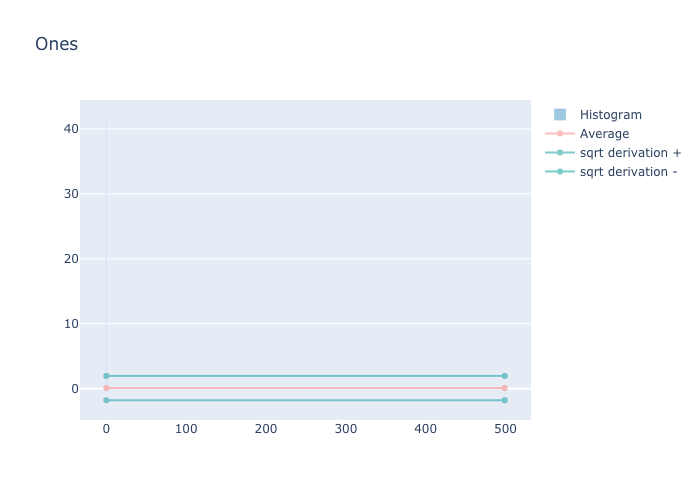
\includegraphics[width=0.6\textwidth]{Images/0/dia-b.png}
          \caption{8\%}
        \end{subfigure}
        \begin{subfigure}[b]{0.4\linewidth}
          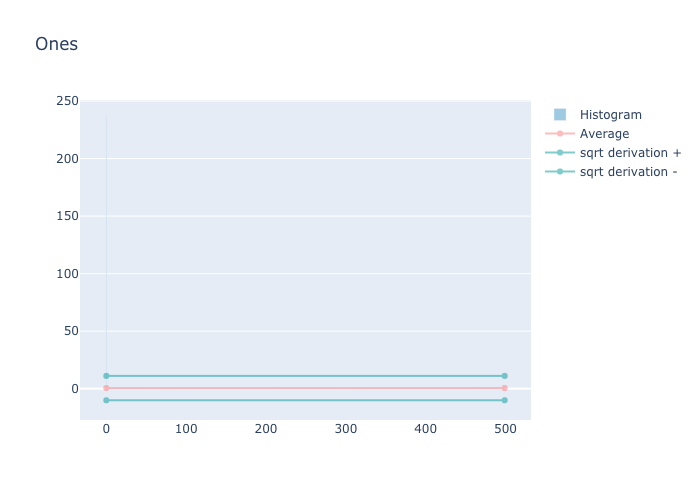
\includegraphics[width=0.6\textwidth]{Images/0/dia-c.png}
          \caption{50\%}
        \end{subfigure}
        \begin{subfigure}[b]{0.4\linewidth}
          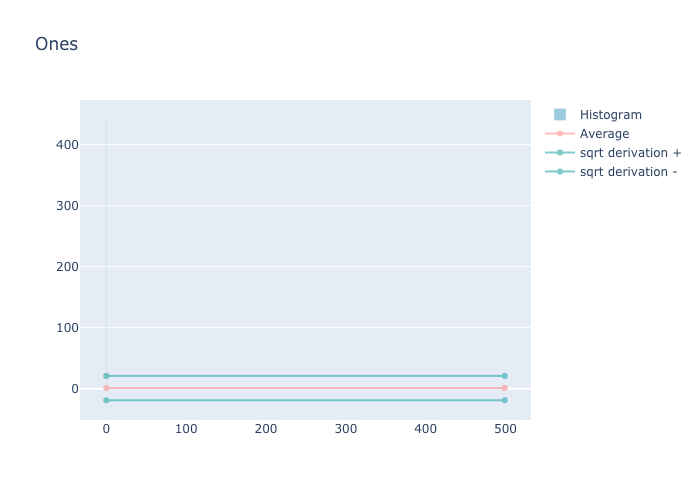
\includegraphics[width=0.6\textwidth]{Images/0/dia-d.png}
          \caption{87\%}
        \end{subfigure}
      \end{figure}


      \clearpage
      \subsection{8}
      \begin{figure}[ht!]
        \centering
        \begin{subfigure}[b]{0.4\linewidth}
          
\includegraphics[width=0.6\textwidth]{Images/8/a.png}
          \caption{One}
        \end{subfigure}
        \begin{subfigure}[b]{0.4\linewidth}
          
\includegraphics[width=0.6\textwidth]{Images/8/b.png}
          \caption{8\%}
        \end{subfigure}
        \begin{subfigure}[b]{0.4\linewidth}
          
\includegraphics[width=0.6\textwidth]{Images/8/c.png}
          \caption{50\%}
        \end{subfigure}
        \begin{subfigure}[b]{0.4\linewidth}
          
\includegraphics[width=0.6\textwidth]{Images/8/d.png}
          \caption{87\%}
        \end{subfigure}
      \end{figure}

      \begin{figure}[ht!]
        \centering
        \begin{subfigure}[b]{0.4\linewidth}
          \includegraphics[width=0.6\textwidth]{Images/8/dia-a.png}
          \caption{One}
        \end{subfigure}
        \begin{subfigure}[b]{0.4\linewidth}
          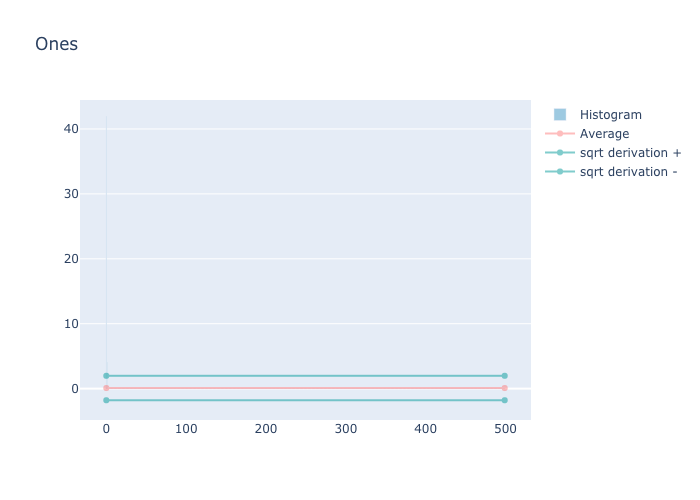
\includegraphics[width=0.6\textwidth]{Images/8/dia-b.png}
          \caption{8\%}
        \end{subfigure}
        \begin{subfigure}[b]{0.4\linewidth}
          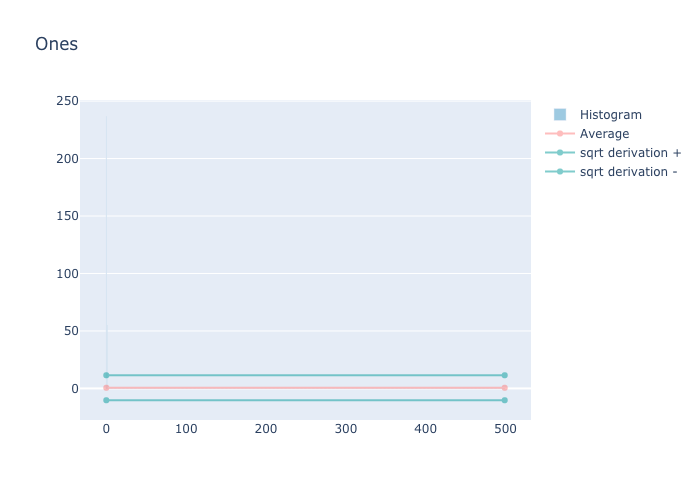
\includegraphics[width=0.6\textwidth]{Images/8/dia-c.png}
          \caption{50\%}
        \end{subfigure}
        \begin{subfigure}[b]{0.4\linewidth}
          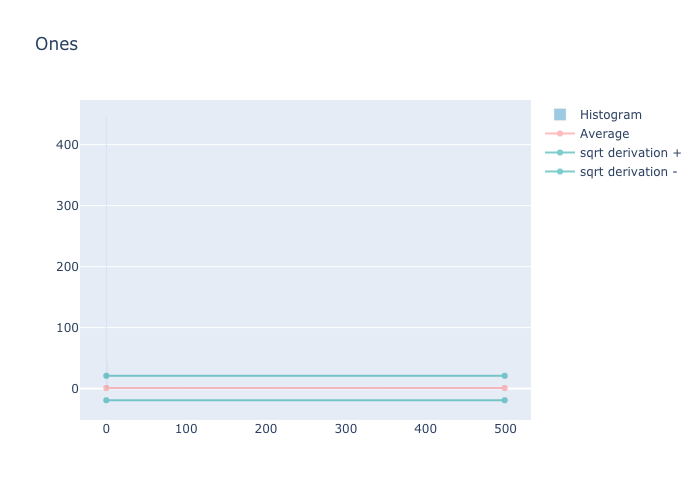
\includegraphics[width=0.6\textwidth]{Images/8/dia-d.png}
          \caption{87\%}
        \end{subfigure}
      \end{figure}


      \clearpage
      \subsection{32}
      \begin{figure}[ht!]
        \centering
        \begin{subfigure}[b]{0.4\linewidth}
          
\includegraphics[width=0.6\textwidth]{Images/32/a.png}
          \caption{One}
        \end{subfigure}
        \begin{subfigure}[b]{0.4\linewidth}
          
\includegraphics[width=0.6\textwidth]{Images/32/b.png}
          \caption{8\%}
        \end{subfigure}
        \begin{subfigure}[b]{0.4\linewidth}
          
\includegraphics[width=0.6\textwidth]{Images/32/c.png}
          \caption{50\%}
        \end{subfigure}
        \begin{subfigure}[b]{0.4\linewidth}
          
\includegraphics[width=0.6\textwidth]{Images/32/d.png}
          \caption{87\%}
        \end{subfigure}
      \end{figure}

      \begin{figure}[ht!]
        \centering
        \begin{subfigure}[b]{0.4\linewidth}
          \includegraphics[width=0.6\textwidth]{Images/32/dia-a.png}
          \caption{One}
        \end{subfigure}
        \begin{subfigure}[b]{0.4\linewidth}
          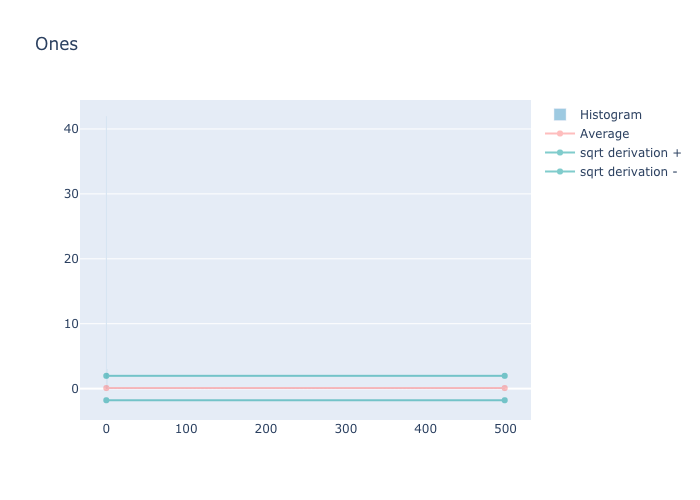
\includegraphics[width=0.6\textwidth]{Images/32/dia-b.png}
          \caption{8\%}
        \end{subfigure}
        \begin{subfigure}[b]{0.4\linewidth}
          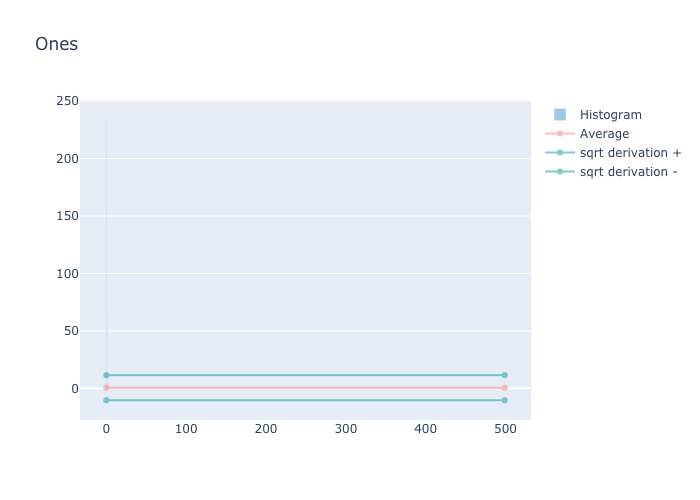
\includegraphics[width=0.6\textwidth]{Images/32/dia-c.png}
          \caption{50\%}
        \end{subfigure}
        \begin{subfigure}[b]{0.4\linewidth}
          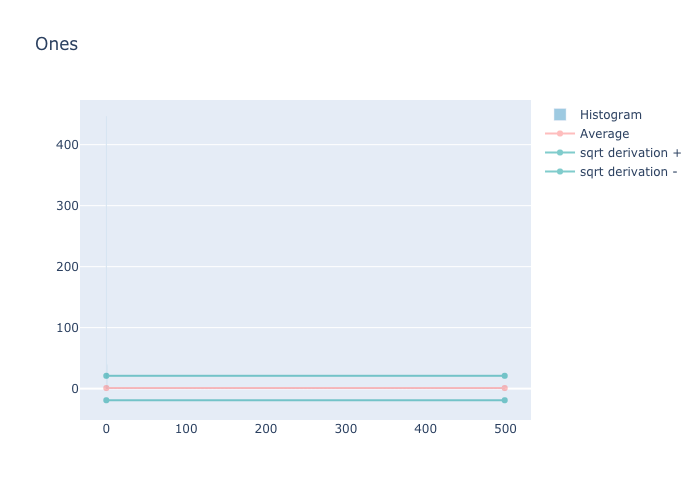
\includegraphics[width=0.6\textwidth]{Images/32/dia-d.png}
          \caption{87\%}
        \end{subfigure}
      \end{figure}


      \clearpage
      \subsection{40}
      \begin{figure}[ht!]
        \centering
        \begin{subfigure}[b]{0.4\linewidth}
          
\includegraphics[width=0.6\textwidth]{Images/40/a.png}
          \caption{One}
        \end{subfigure}
        \begin{subfigure}[b]{0.4\linewidth}
          
\includegraphics[width=0.6\textwidth]{Images/40/b.png}
          \caption{8\%}
        \end{subfigure}
        \begin{subfigure}[b]{0.4\linewidth}
          
\includegraphics[width=0.6\textwidth]{Images/40/c.png}
          \caption{50\%}
        \end{subfigure}
        \begin{subfigure}[b]{0.4\linewidth}
          
\includegraphics[width=0.6\textwidth]{Images/40/d.png}
          \caption{87\%}
        \end{subfigure}
      \end{figure}

      \begin{figure}[ht!]
        \centering
        \begin{subfigure}[b]{0.4\linewidth}
          \includegraphics[width=0.6\textwidth]{Images/40/dia-a.png}
          \caption{One}
        \end{subfigure}
        \begin{subfigure}[b]{0.4\linewidth}
          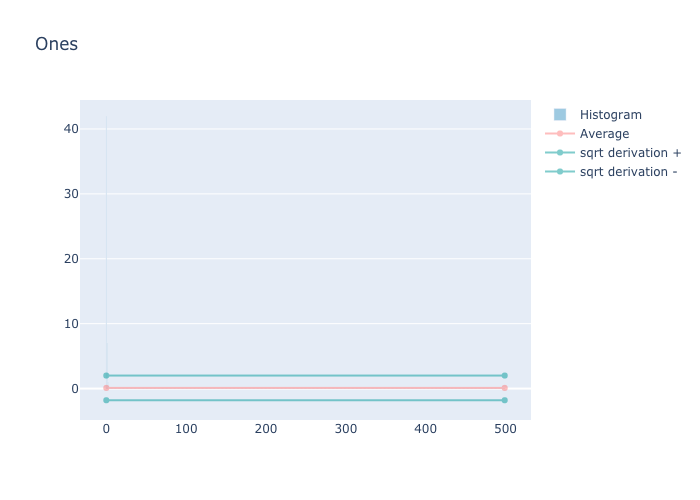
\includegraphics[width=0.6\textwidth]{Images/40/dia-b.png}
          \caption{8\%}
        \end{subfigure}
        \begin{subfigure}[b]{0.4\linewidth}
          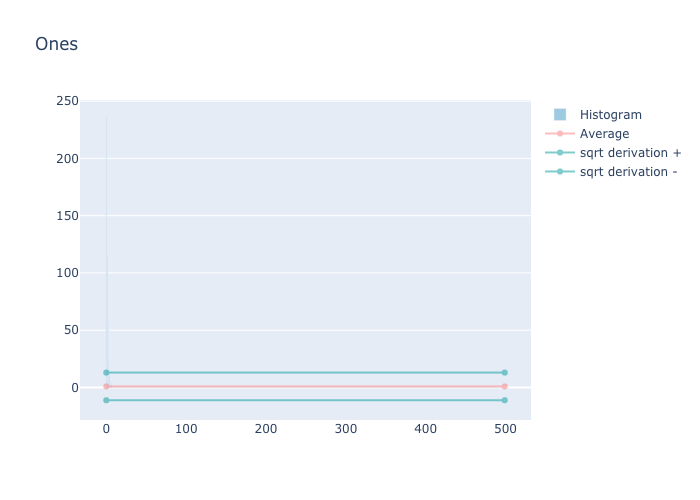
\includegraphics[width=0.6\textwidth]{Images/40/dia-c.png}
          \caption{50\%}
        \end{subfigure}
        \begin{subfigure}[b]{0.4\linewidth}
          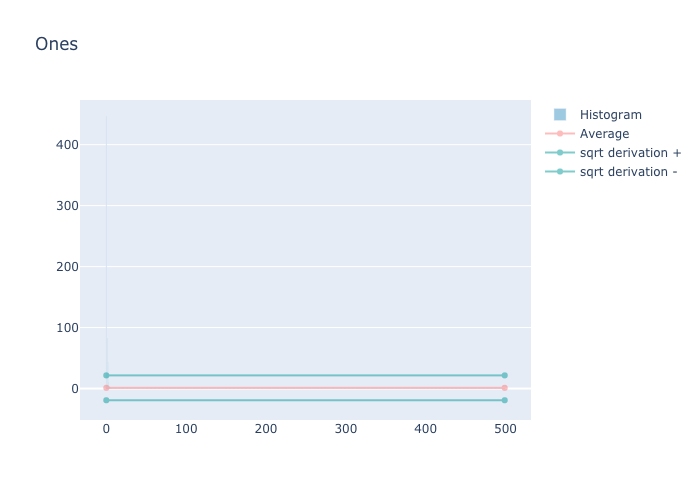
\includegraphics[width=0.6\textwidth]{Images/40/dia-d.png}
          \caption{87\%}
        \end{subfigure}
      \end{figure}


      \clearpage
      \subsection{128}
      \begin{figure}[ht!]
        \centering
        \begin{subfigure}[b]{0.4\linewidth}
          
\includegraphics[width=0.6\textwidth]{Images/128/a.png}
          \caption{One}
        \end{subfigure}
        \begin{subfigure}[b]{0.4\linewidth}
          
\includegraphics[width=0.6\textwidth]{Images/128/b.png}
          \caption{8\%}
        \end{subfigure}
        \begin{subfigure}[b]{0.4\linewidth}
          
\includegraphics[width=0.6\textwidth]{Images/128/c.png}
          \caption{50\%}
        \end{subfigure}
        \begin{subfigure}[b]{0.4\linewidth}
          
\includegraphics[width=0.6\textwidth]{Images/128/d.png}
          \caption{87\%}
        \end{subfigure}
      \end{figure}

      \begin{figure}[ht!]
        \centering
        \begin{subfigure}[b]{0.4\linewidth}
          \includegraphics[width=0.6\textwidth]{Images/128/dia-a.png}
          \caption{One}
        \end{subfigure}
        \begin{subfigure}[b]{0.4\linewidth}
          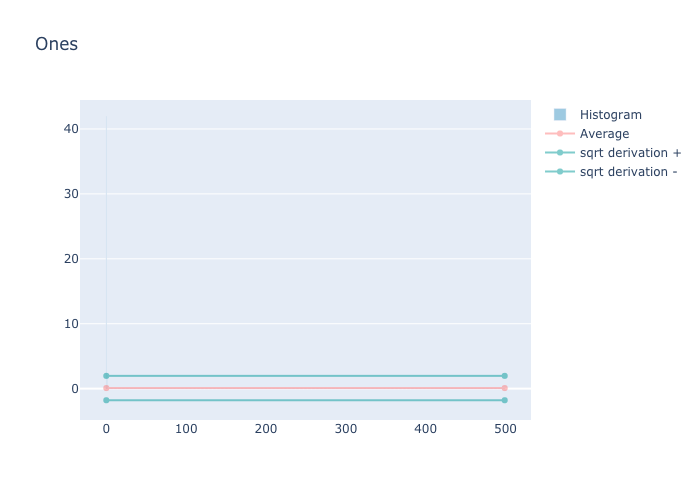
\includegraphics[width=0.6\textwidth]{Images/128/dia-b.png}
          \caption{8\%}
        \end{subfigure}
        \begin{subfigure}[b]{0.4\linewidth}
          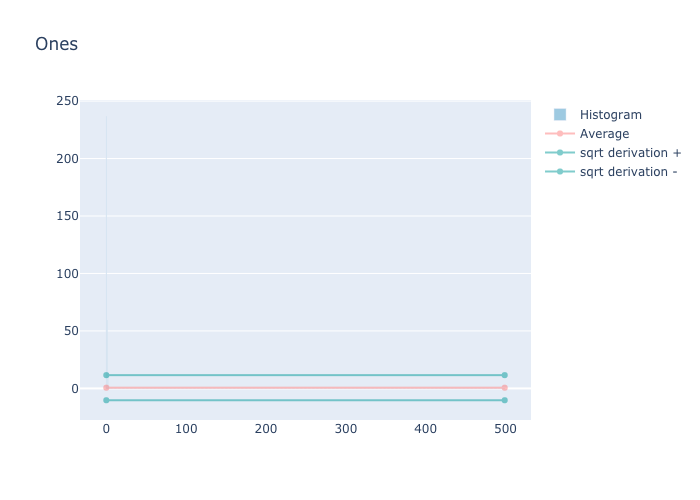
\includegraphics[width=0.6\textwidth]{Images/128/dia-c.png}
          \caption{50\%}
        \end{subfigure}
        \begin{subfigure}[b]{0.4\linewidth}
          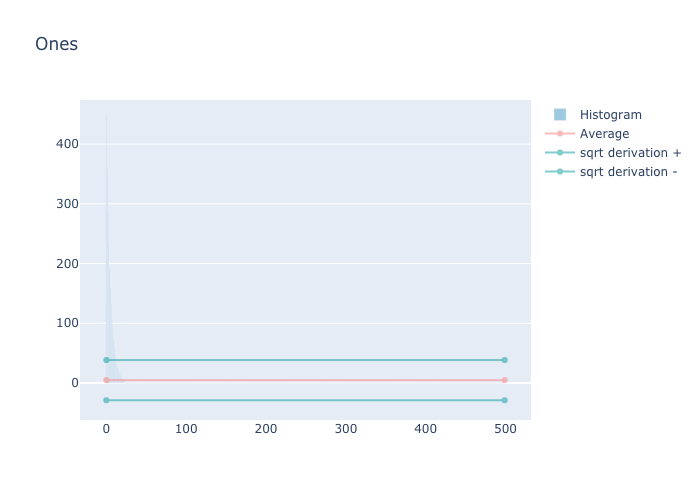
\includegraphics[width=0.6\textwidth]{Images/128/dia-d.png}
          \caption{87\%}
        \end{subfigure}
      \end{figure}


      \clearpage
      \subsection{136}
      \begin{figure}[ht!]
        \centering
        \begin{subfigure}[b]{0.4\linewidth}
          
\includegraphics[width=0.6\textwidth]{Images/136/a.png}
          \caption{One}
        \end{subfigure}
        \begin{subfigure}[b]{0.4\linewidth}
          
\includegraphics[width=0.6\textwidth]{Images/136/b.png}
          \caption{8\%}
        \end{subfigure}
        \begin{subfigure}[b]{0.4\linewidth}
          
\includegraphics[width=0.6\textwidth]{Images/136/c.png}
          \caption{50\%}
        \end{subfigure}
        \begin{subfigure}[b]{0.4\linewidth}
          
\includegraphics[width=0.6\textwidth]{Images/136/d.png}
          \caption{87\%}
        \end{subfigure}
      \end{figure}

      \begin{figure}[ht!]
        \centering
        \begin{subfigure}[b]{0.4\linewidth}
          \includegraphics[width=0.6\textwidth]{Images/136/dia-a.png}
          \caption{One}
        \end{subfigure}
        \begin{subfigure}[b]{0.4\linewidth}
          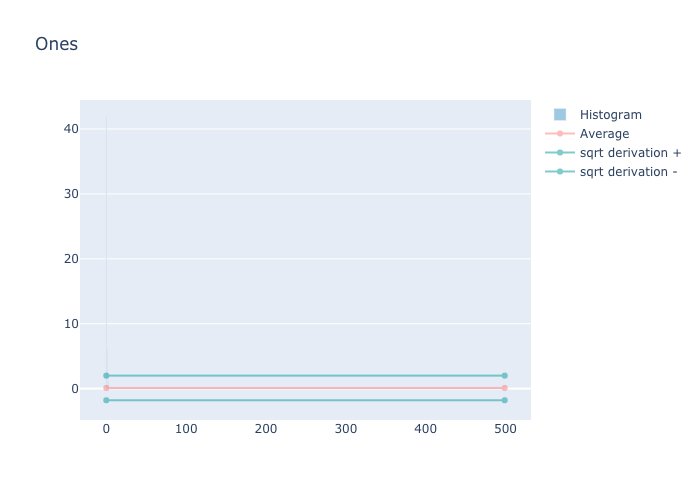
\includegraphics[width=0.6\textwidth]{Images/136/dia-b.png}
          \caption{8\%}
        \end{subfigure}
        \begin{subfigure}[b]{0.4\linewidth}
          \includegraphics[width=0.6\textwidth]{Images/136/dia-c.png}
          \caption{50\%}
        \end{subfigure}
        \begin{subfigure}[b]{0.4\linewidth}
          \includegraphics[width=0.6\textwidth]{Images/136/dia-d.png}
          \caption{87\%}
        \end{subfigure}
      \end{figure}


      \clearpage
      \subsection{160}
      \begin{figure}[ht!]
        \centering
        \begin{subfigure}[b]{0.4\linewidth}
          \includegraphics[width=0.6\textwidth]{Images/160/a.png}
          \caption{One}
        \end{subfigure}
        \begin{subfigure}[b]{0.4\linewidth}
          \includegraphics[width=0.6\textwidth]{Images/160/b.png}
          \caption{8\%}
        \end{subfigure}
        \begin{subfigure}[b]{0.4\linewidth}
          \includegraphics[width=0.6\textwidth]{Images/160/c.png}
          \caption{50\%}
        \end{subfigure}
        \begin{subfigure}[b]{0.4\linewidth}
          \includegraphics[width=0.6\textwidth]{Images/160/d.png}
          \caption{87\%}
        \end{subfigure}
      \end{figure}

      \begin{figure}[ht!]
        \centering
        \begin{subfigure}[b]{0.4\linewidth}
          \includegraphics[width=0.6\textwidth]{Images/160/dia-a.png}
          \caption{One}
        \end{subfigure}
        \begin{subfigure}[b]{0.4\linewidth}
          \includegraphics[width=0.6\textwidth]{Images/160/dia-b.png}
          \caption{8\%}
        \end{subfigure}
        \begin{subfigure}[b]{0.4\linewidth}
          \includegraphics[width=0.6\textwidth]{Images/160/dia-c.png}
          \caption{50\%}
        \end{subfigure}
        \begin{subfigure}[b]{0.4\linewidth}
          \includegraphics[width=0.6\textwidth]{Images/160/dia-d.png}
          \caption{87\%}
        \end{subfigure}
      \end{figure}


      \clearpage
      \subsection{168}
      \begin{figure}[ht!]
        \centering
        \begin{subfigure}[b]{0.4\linewidth}
          \includegraphics[width=0.6\textwidth]{Images/168/a.png}
          \caption{One}
        \end{subfigure}
        \begin{subfigure}[b]{0.4\linewidth}
          \includegraphics[width=0.6\textwidth]{Images/168/b.png}
          \caption{8\%}
        \end{subfigure}
        \begin{subfigure}[b]{0.4\linewidth}
          \includegraphics[width=0.6\textwidth]{Images/168/c.png}
          \caption{50\%}
        \end{subfigure}
        \begin{subfigure}[b]{0.4\linewidth}
          \includegraphics[width=0.6\textwidth]{Images/168/d.png}
          \caption{87\%}
        \end{subfigure}
      \end{figure}

      \begin{figure}[ht!]
        \centering
        \begin{subfigure}[b]{0.4\linewidth}
          \includegraphics[width=0.6\textwidth]{Images/168/dia-a.png}
          \caption{One}
        \end{subfigure}
        \begin{subfigure}[b]{0.4\linewidth}
          \includegraphics[width=0.6\textwidth]{Images/168/dia-b.png}
          \caption{8\%}
        \end{subfigure}
        \begin{subfigure}[b]{0.4\linewidth}
          \includegraphics[width=0.6\textwidth]{Images/168/dia-c.png}
          \caption{50\%}
        \end{subfigure}
        \begin{subfigure}[b]{0.4\linewidth}
          \includegraphics[width=0.6\textwidth]{Images/168/dia-d.png}
          \caption{87\%}
        \end{subfigure}
      \end{figure}























      % =====================================================
      % ========                W2                  =========
      % =====================================================
      \clearpage
      \section{W2}
              

       

            
      \subsection{1}
      \begin{figure}[ht!]
        \centering
        \begin{subfigure}[b]{0.4\linewidth}
          \includegraphics[width=0.6\textwidth]{Images/1/a.png}
          \caption{One}
        \end{subfigure}
        \begin{subfigure}[b]{0.4\linewidth}
          \includegraphics[width=0.6\textwidth]{Images/1/b.png}
          \caption{8\%}
        \end{subfigure}
        \begin{subfigure}[b]{0.4\linewidth}
          \includegraphics[width=0.6\textwidth]{Images/1/c.png}
          \caption{50\%}
        \end{subfigure}
        \begin{subfigure}[b]{0.4\linewidth}
          \includegraphics[width=0.6\textwidth]{Images/1/d.png}
          \caption{87\%}
        \end{subfigure}
      \end{figure}

      \begin{figure}[ht!]
        \centering
        \begin{subfigure}[b]{0.4\linewidth}
          \includegraphics[width=0.6\textwidth]{Images/1/dia-a.png}
          \caption{One}
        \end{subfigure}
        \begin{subfigure}[b]{0.4\linewidth}
          \includegraphics[width=0.6\textwidth]{Images/1/dia-b.png}
          \caption{8\%}
        \end{subfigure}
        \begin{subfigure}[b]{0.4\linewidth}
          \includegraphics[width=0.6\textwidth]{Images/1/dia-c.png}
          \caption{50\%}
        \end{subfigure}
        \begin{subfigure}[b]{0.4\linewidth}
          \includegraphics[width=0.6\textwidth]{Images/1/dia-d.png}
          \caption{87\%}
        \end{subfigure}
      \end{figure}


      \clearpage
      \subsection{2}
      \begin{figure}[ht!]
        \centering
        \begin{subfigure}[b]{0.4\linewidth}
          \includegraphics[width=0.6\textwidth]{Images/2/a.png}
          \caption{One}
        \end{subfigure}
        \begin{subfigure}[b]{0.4\linewidth}
          \includegraphics[width=0.6\textwidth]{Images/2/b.png}
          \caption{8\%}
        \end{subfigure}
        \begin{subfigure}[b]{0.4\linewidth}
          \includegraphics[width=0.6\textwidth]{Images/2/c.png}
          \caption{50\%}
        \end{subfigure}
        \begin{subfigure}[b]{0.4\linewidth}
          \includegraphics[width=0.6\textwidth]{Images/2/d.png}
          \caption{87\%}
        \end{subfigure}
      \end{figure}

      \begin{figure}[ht!]
        \centering
        \begin{subfigure}[b]{0.4\linewidth}
          \includegraphics[width=0.6\textwidth]{Images/2/dia-a.png}
          \caption{One}
        \end{subfigure}
        \begin{subfigure}[b]{0.4\linewidth}
          \includegraphics[width=0.6\textwidth]{Images/2/dia-b.png}
          \caption{8\%}
        \end{subfigure}
        \begin{subfigure}[b]{0.4\linewidth}
          \includegraphics[width=0.6\textwidth]{Images/2/dia-c.png}
          \caption{50\%}
        \end{subfigure}
        \begin{subfigure}[b]{0.4\linewidth}
          \includegraphics[width=0.6\textwidth]{Images/2/dia-d.png}
          \caption{87\%}
        \end{subfigure}
      \end{figure}


      \clearpage
      \subsection{3}
      \begin{figure}[ht!]
        \centering
        \begin{subfigure}[b]{0.4\linewidth}
          \includegraphics[width=0.6\textwidth]{Images/3/a.png}
          \caption{One}
        \end{subfigure}
        \begin{subfigure}[b]{0.4\linewidth}
          \includegraphics[width=0.6\textwidth]{Images/3/b.png}
          \caption{8\%}
        \end{subfigure}
        \begin{subfigure}[b]{0.4\linewidth}
          \includegraphics[width=0.6\textwidth]{Images/3/c.png}
          \caption{50\%}
        \end{subfigure}
        \begin{subfigure}[b]{0.4\linewidth}
          \includegraphics[width=0.6\textwidth]{Images/3/d.png}
          \caption{87\%}
        \end{subfigure}
      \end{figure}

      \begin{figure}[ht!]
        \centering
        \begin{subfigure}[b]{0.4\linewidth}
          \includegraphics[width=0.6\textwidth]{Images/3/dia-a.png}
          \caption{One}
        \end{subfigure}
        \begin{subfigure}[b]{0.4\linewidth}
          \includegraphics[width=0.6\textwidth]{Images/3/dia-b.png}
          \caption{8\%}
        \end{subfigure}
        \begin{subfigure}[b]{0.4\linewidth}
          \includegraphics[width=0.6\textwidth]{Images/3/dia-c.png}
          \caption{50\%}
        \end{subfigure}
        \begin{subfigure}[b]{0.4\linewidth}
          \includegraphics[width=0.6\textwidth]{Images/3/dia-d.png}
          \caption{87\%}
        \end{subfigure}
      \end{figure}


      \clearpage
      \subsection{4}
      \begin{figure}[ht!]
        \centering
        \begin{subfigure}[b]{0.4\linewidth}
          \includegraphics[width=0.6\textwidth]{Images/4/a.png}
          \caption{One}
        \end{subfigure}
        \begin{subfigure}[b]{0.4\linewidth}
          \includegraphics[width=0.6\textwidth]{Images/4/b.png}
          \caption{8\%}
        \end{subfigure}
        \begin{subfigure}[b]{0.4\linewidth}
          \includegraphics[width=0.6\textwidth]{Images/4/c.png}
          \caption{50\%}
        \end{subfigure}
        \begin{subfigure}[b]{0.4\linewidth}
          \includegraphics[width=0.6\textwidth]{Images/4/d.png}
          \caption{87\%}
        \end{subfigure}
      \end{figure}

      \begin{figure}[ht!]
        \centering
        \begin{subfigure}[b]{0.4\linewidth}
          \includegraphics[width=0.6\textwidth]{Images/4/dia-a.png}
          \caption{One}
        \end{subfigure}
        \begin{subfigure}[b]{0.4\linewidth}
          \includegraphics[width=0.6\textwidth]{Images/4/dia-b.png}
          \caption{8\%}
        \end{subfigure}
        \begin{subfigure}[b]{0.4\linewidth}
          \includegraphics[width=0.6\textwidth]{Images/4/dia-c.png}
          \caption{50\%}
        \end{subfigure}
        \begin{subfigure}[b]{0.4\linewidth}
          \includegraphics[width=0.6\textwidth]{Images/4/dia-d.png}
          \caption{87\%}
        \end{subfigure}
      \end{figure}


      \clearpage
      \subsection{5}
      \begin{figure}[ht!]
        \centering
        \begin{subfigure}[b]{0.4\linewidth}
          \includegraphics[width=0.6\textwidth]{Images/5/a.png}
          \caption{One}
        \end{subfigure}
        \begin{subfigure}[b]{0.4\linewidth}
          \includegraphics[width=0.6\textwidth]{Images/5/b.png}
          \caption{8\%}
        \end{subfigure}
        \begin{subfigure}[b]{0.4\linewidth}
          \includegraphics[width=0.6\textwidth]{Images/5/c.png}
          \caption{50\%}
        \end{subfigure}
        \begin{subfigure}[b]{0.4\linewidth}
          \includegraphics[width=0.6\textwidth]{Images/5/d.png}
          \caption{87\%}
        \end{subfigure}
      \end{figure}

      \begin{figure}[ht!]
        \centering
        \begin{subfigure}[b]{0.4\linewidth}
          \includegraphics[width=0.6\textwidth]{Images/5/dia-a.png}
          \caption{One}
        \end{subfigure}
        \begin{subfigure}[b]{0.4\linewidth}
          \includegraphics[width=0.6\textwidth]{Images/5/dia-b.png}
          \caption{8\%}
        \end{subfigure}
        \begin{subfigure}[b]{0.4\linewidth}
          \includegraphics[width=0.6\textwidth]{Images/5/dia-c.png}
          \caption{50\%}
        \end{subfigure}
        \begin{subfigure}[b]{0.4\linewidth}
          \includegraphics[width=0.6\textwidth]{Images/5/dia-d.png}
          \caption{87\%}
        \end{subfigure}
      \end{figure}


      \clearpage
      \subsection{6}
      \begin{figure}[ht!]
        \centering
        \begin{subfigure}[b]{0.4\linewidth}
          \includegraphics[width=0.6\textwidth]{Images/6/a.png}
          \caption{One}
        \end{subfigure}
        \begin{subfigure}[b]{0.4\linewidth}
          \includegraphics[width=0.6\textwidth]{Images/6/b.png}
          \caption{8\%}
        \end{subfigure}
        \begin{subfigure}[b]{0.4\linewidth}
          \includegraphics[width=0.6\textwidth]{Images/6/c.png}
          \caption{50\%}
        \end{subfigure}
        \begin{subfigure}[b]{0.4\linewidth}
          \includegraphics[width=0.6\textwidth]{Images/6/d.png}
          \caption{87\%}
        \end{subfigure}
      \end{figure}

      \begin{figure}[ht!]
        \centering
        \begin{subfigure}[b]{0.4\linewidth}
          \includegraphics[width=0.6\textwidth]{Images/6/dia-a.png}
          \caption{One}
        \end{subfigure}
        \begin{subfigure}[b]{0.4\linewidth}
          \includegraphics[width=0.6\textwidth]{Images/6/dia-b.png}
          \caption{8\%}
        \end{subfigure}
        \begin{subfigure}[b]{0.4\linewidth}
          \includegraphics[width=0.6\textwidth]{Images/6/dia-c.png}
          \caption{50\%}
        \end{subfigure}
        \begin{subfigure}[b]{0.4\linewidth}
          \includegraphics[width=0.6\textwidth]{Images/6/dia-d.png}
          \caption{87\%}
        \end{subfigure}
      \end{figure}


      \clearpage
      \subsection{7}
      \begin{figure}[ht!]
        \centering
        \begin{subfigure}[b]{0.4\linewidth}
          \includegraphics[width=0.6\textwidth]{Images/7/a.png}
          \caption{One}
        \end{subfigure}
        \begin{subfigure}[b]{0.4\linewidth}
          \includegraphics[width=0.6\textwidth]{Images/7/b.png}
          \caption{8\%}
        \end{subfigure}
        \begin{subfigure}[b]{0.4\linewidth}
          \includegraphics[width=0.6\textwidth]{Images/7/c.png}
          \caption{50\%}
        \end{subfigure}
        \begin{subfigure}[b]{0.4\linewidth}
          \includegraphics[width=0.6\textwidth]{Images/7/d.png}
          \caption{87\%}
        \end{subfigure}
      \end{figure}

      \begin{figure}[ht!]
        \centering
        \begin{subfigure}[b]{0.4\linewidth}
          \includegraphics[width=0.6\textwidth]{Images/7/dia-a.png}
          \caption{One}
        \end{subfigure}
        \begin{subfigure}[b]{0.4\linewidth}
          \includegraphics[width=0.6\textwidth]{Images/7/dia-b.png}
          \caption{8\%}
        \end{subfigure}
        \begin{subfigure}[b]{0.4\linewidth}
          \includegraphics[width=0.6\textwidth]{Images/7/dia-c.png}
          \caption{50\%}
        \end{subfigure}
        \begin{subfigure}[b]{0.4\linewidth}
          \includegraphics[width=0.6\textwidth]{Images/7/dia-d.png}
          \caption{87\%}
        \end{subfigure}
      \end{figure}


      \clearpage
      \subsection{9}
      \begin{figure}[ht!]
        \centering
        \begin{subfigure}[b]{0.4\linewidth}
          \includegraphics[width=0.6\textwidth]{Images/9/a.png}
          \caption{One}
        \end{subfigure}
        \begin{subfigure}[b]{0.4\linewidth}
          \includegraphics[width=0.6\textwidth]{Images/9/b.png}
          \caption{8\%}
        \end{subfigure}
        \begin{subfigure}[b]{0.4\linewidth}
          \includegraphics[width=0.6\textwidth]{Images/9/c.png}
          \caption{50\%}
        \end{subfigure}
        \begin{subfigure}[b]{0.4\linewidth}
          \includegraphics[width=0.6\textwidth]{Images/9/d.png}
          \caption{87\%}
        \end{subfigure}
      \end{figure}

      \begin{figure}[ht!]
        \centering
        \begin{subfigure}[b]{0.4\linewidth}
          \includegraphics[width=0.6\textwidth]{Images/9/dia-a.png}
          \caption{One}
        \end{subfigure}
        \begin{subfigure}[b]{0.4\linewidth}
          \includegraphics[width=0.6\textwidth]{Images/9/dia-b.png}
          \caption{8\%}
        \end{subfigure}
        \begin{subfigure}[b]{0.4\linewidth}
          \includegraphics[width=0.6\textwidth]{Images/9/dia-c.png}
          \caption{50\%}
        \end{subfigure}
        \begin{subfigure}[b]{0.4\linewidth}
          \includegraphics[width=0.6\textwidth]{Images/9/dia-d.png}
          \caption{87\%}
        \end{subfigure}
      \end{figure}


      \clearpage
      \subsection{10}
      \begin{figure}[ht!]
        \centering
        \begin{subfigure}[b]{0.4\linewidth}
          \includegraphics[width=0.6\textwidth]{Images/10/a.png}
          \caption{One}
        \end{subfigure}
        \begin{subfigure}[b]{0.4\linewidth}
          \includegraphics[width=0.6\textwidth]{Images/10/b.png}
          \caption{8\%}
        \end{subfigure}
        \begin{subfigure}[b]{0.4\linewidth}
          \includegraphics[width=0.6\textwidth]{Images/10/c.png}
          \caption{50\%}
        \end{subfigure}
        \begin{subfigure}[b]{0.4\linewidth}
          \includegraphics[width=0.6\textwidth]{Images/10/d.png}
          \caption{87\%}
        \end{subfigure}
      \end{figure}

      \begin{figure}[ht!]
        \centering
        \begin{subfigure}[b]{0.4\linewidth}
          \includegraphics[width=0.6\textwidth]{Images/10/dia-a.png}
          \caption{One}
        \end{subfigure}
        \begin{subfigure}[b]{0.4\linewidth}
          \includegraphics[width=0.6\textwidth]{Images/10/dia-b.png}
          \caption{8\%}
        \end{subfigure}
        \begin{subfigure}[b]{0.4\linewidth}
          \includegraphics[width=0.6\textwidth]{Images/10/dia-c.png}
          \caption{50\%}
        \end{subfigure}
        \begin{subfigure}[b]{0.4\linewidth}
          \includegraphics[width=0.6\textwidth]{Images/10/dia-d.png}
          \caption{87\%}
        \end{subfigure}
      \end{figure}


      \clearpage
      \subsection{11}
      \begin{figure}[ht!]
        \centering
        \begin{subfigure}[b]{0.4\linewidth}
          \includegraphics[width=0.6\textwidth]{Images/11/a.png}
          \caption{One}
        \end{subfigure}
        \begin{subfigure}[b]{0.4\linewidth}
          \includegraphics[width=0.6\textwidth]{Images/11/b.png}
          \caption{8\%}
        \end{subfigure}
        \begin{subfigure}[b]{0.4\linewidth}
          \includegraphics[width=0.6\textwidth]{Images/11/c.png}
          \caption{50\%}
        \end{subfigure}
        \begin{subfigure}[b]{0.4\linewidth}
          \includegraphics[width=0.6\textwidth]{Images/11/d.png}
          \caption{87\%}
        \end{subfigure}
      \end{figure}

      \begin{figure}[ht!]
        \centering
        \begin{subfigure}[b]{0.4\linewidth}
          \includegraphics[width=0.6\textwidth]{Images/11/dia-a.png}
          \caption{One}
        \end{subfigure}
        \begin{subfigure}[b]{0.4\linewidth}
          \includegraphics[width=0.6\textwidth]{Images/11/dia-b.png}
          \caption{8\%}
        \end{subfigure}
        \begin{subfigure}[b]{0.4\linewidth}
          \includegraphics[width=0.6\textwidth]{Images/11/dia-c.png}
          \caption{50\%}
        \end{subfigure}
        \begin{subfigure}[b]{0.4\linewidth}
          \includegraphics[width=0.6\textwidth]{Images/11/dia-d.png}
          \caption{87\%}
        \end{subfigure}
      \end{figure}


      \clearpage
      \subsection{12}
      \begin{figure}[ht!]
        \centering
        \begin{subfigure}[b]{0.4\linewidth}
          \includegraphics[width=0.6\textwidth]{Images/12/a.png}
          \caption{One}
        \end{subfigure}
        \begin{subfigure}[b]{0.4\linewidth}
          \includegraphics[width=0.6\textwidth]{Images/12/b.png}
          \caption{8\%}
        \end{subfigure}
        \begin{subfigure}[b]{0.4\linewidth}
          \includegraphics[width=0.6\textwidth]{Images/12/c.png}
          \caption{50\%}
        \end{subfigure}
        \begin{subfigure}[b]{0.4\linewidth}
          \includegraphics[width=0.6\textwidth]{Images/12/d.png}
          \caption{87\%}
        \end{subfigure}
      \end{figure}

      \begin{figure}[ht!]
        \centering
        \begin{subfigure}[b]{0.4\linewidth}
          \includegraphics[width=0.6\textwidth]{Images/12/dia-a.png}
          \caption{One}
        \end{subfigure}
        \begin{subfigure}[b]{0.4\linewidth}
          \includegraphics[width=0.6\textwidth]{Images/12/dia-b.png}
          \caption{8\%}
        \end{subfigure}
        \begin{subfigure}[b]{0.4\linewidth}
          \includegraphics[width=0.6\textwidth]{Images/12/dia-c.png}
          \caption{50\%}
        \end{subfigure}
        \begin{subfigure}[b]{0.4\linewidth}
          \includegraphics[width=0.6\textwidth]{Images/12/dia-d.png}
          \caption{87\%}
        \end{subfigure}
      \end{figure}


      \clearpage
      \subsection{13}
      \begin{figure}[ht!]
        \centering
        \begin{subfigure}[b]{0.4\linewidth}
          \includegraphics[width=0.6\textwidth]{Images/13/a.png}
          \caption{One}
        \end{subfigure}
        \begin{subfigure}[b]{0.4\linewidth}
          \includegraphics[width=0.6\textwidth]{Images/13/b.png}
          \caption{8\%}
        \end{subfigure}
        \begin{subfigure}[b]{0.4\linewidth}
          \includegraphics[width=0.6\textwidth]{Images/13/c.png}
          \caption{50\%}
        \end{subfigure}
        \begin{subfigure}[b]{0.4\linewidth}
          \includegraphics[width=0.6\textwidth]{Images/13/d.png}
          \caption{87\%}
        \end{subfigure}
      \end{figure}

      \begin{figure}[ht!]
        \centering
        \begin{subfigure}[b]{0.4\linewidth}
          \includegraphics[width=0.6\textwidth]{Images/13/dia-a.png}
          \caption{One}
        \end{subfigure}
        \begin{subfigure}[b]{0.4\linewidth}
          \includegraphics[width=0.6\textwidth]{Images/13/dia-b.png}
          \caption{8\%}
        \end{subfigure}
        \begin{subfigure}[b]{0.4\linewidth}
          \includegraphics[width=0.6\textwidth]{Images/13/dia-c.png}
          \caption{50\%}
        \end{subfigure}
        \begin{subfigure}[b]{0.4\linewidth}
          \includegraphics[width=0.6\textwidth]{Images/13/dia-d.png}
          \caption{87\%}
        \end{subfigure}
      \end{figure}


      \clearpage
      \subsection{14}
      \begin{figure}[ht!]
        \centering
        \begin{subfigure}[b]{0.4\linewidth}
          \includegraphics[width=0.6\textwidth]{Images/14/a.png}
          \caption{One}
        \end{subfigure}
        \begin{subfigure}[b]{0.4\linewidth}
          \includegraphics[width=0.6\textwidth]{Images/14/b.png}
          \caption{8\%}
        \end{subfigure}
        \begin{subfigure}[b]{0.4\linewidth}
          \includegraphics[width=0.6\textwidth]{Images/14/c.png}
          \caption{50\%}
        \end{subfigure}
        \begin{subfigure}[b]{0.4\linewidth}
          \includegraphics[width=0.6\textwidth]{Images/14/d.png}
          \caption{87\%}
        \end{subfigure}
      \end{figure}

      \begin{figure}[ht!]
        \centering
        \begin{subfigure}[b]{0.4\linewidth}
          \includegraphics[width=0.6\textwidth]{Images/14/dia-a.png}
          \caption{One}
        \end{subfigure}
        \begin{subfigure}[b]{0.4\linewidth}
          \includegraphics[width=0.6\textwidth]{Images/14/dia-b.png}
          \caption{8\%}
        \end{subfigure}
        \begin{subfigure}[b]{0.4\linewidth}
          \includegraphics[width=0.6\textwidth]{Images/14/dia-c.png}
          \caption{50\%}
        \end{subfigure}
        \begin{subfigure}[b]{0.4\linewidth}
          \includegraphics[width=0.6\textwidth]{Images/14/dia-d.png}
          \caption{87\%}
        \end{subfigure}
      \end{figure}


      \clearpage
      \subsection{15}
      \begin{figure}[ht!]
        \centering
        \begin{subfigure}[b]{0.4\linewidth}
          \includegraphics[width=0.6\textwidth]{Images/15/a.png}
          \caption{One}
        \end{subfigure}
        \begin{subfigure}[b]{0.4\linewidth}
          \includegraphics[width=0.6\textwidth]{Images/15/b.png}
          \caption{8\%}
        \end{subfigure}
        \begin{subfigure}[b]{0.4\linewidth}
          \includegraphics[width=0.6\textwidth]{Images/15/c.png}
          \caption{50\%}
        \end{subfigure}
        \begin{subfigure}[b]{0.4\linewidth}
          \includegraphics[width=0.6\textwidth]{Images/15/d.png}
          \caption{87\%}
        \end{subfigure}
      \end{figure}

      \begin{figure}[ht!]
        \centering
        \begin{subfigure}[b]{0.4\linewidth}
          \includegraphics[width=0.6\textwidth]{Images/15/dia-a.png}
          \caption{One}
        \end{subfigure}
        \begin{subfigure}[b]{0.4\linewidth}
          \includegraphics[width=0.6\textwidth]{Images/15/dia-b.png}
          \caption{8\%}
        \end{subfigure}
        \begin{subfigure}[b]{0.4\linewidth}
          \includegraphics[width=0.6\textwidth]{Images/15/dia-c.png}
          \caption{50\%}
        \end{subfigure}
        \begin{subfigure}[b]{0.4\linewidth}
          \includegraphics[width=0.6\textwidth]{Images/15/dia-d.png}
          \caption{87\%}
        \end{subfigure}
      \end{figure}


      \clearpage
      \subsection{19}
      \begin{figure}[ht!]
        \centering
        \begin{subfigure}[b]{0.4\linewidth}
          \includegraphics[width=0.6\textwidth]{Images/19/a.png}
          \caption{One}
        \end{subfigure}
        \begin{subfigure}[b]{0.4\linewidth}
          \includegraphics[width=0.6\textwidth]{Images/19/b.png}
          \caption{8\%}
        \end{subfigure}
        \begin{subfigure}[b]{0.4\linewidth}
          \includegraphics[width=0.6\textwidth]{Images/19/c.png}
          \caption{50\%}
        \end{subfigure}
        \begin{subfigure}[b]{0.4\linewidth}
          \includegraphics[width=0.6\textwidth]{Images/19/d.png}
          \caption{87\%}
        \end{subfigure}
      \end{figure}

      \begin{figure}[ht!]
        \centering
        \begin{subfigure}[b]{0.4\linewidth}
          \includegraphics[width=0.6\textwidth]{Images/19/dia-a.png}
          \caption{One}
        \end{subfigure}
        \begin{subfigure}[b]{0.4\linewidth}
          \includegraphics[width=0.6\textwidth]{Images/19/dia-b.png}
          \caption{8\%}
        \end{subfigure}
        \begin{subfigure}[b]{0.4\linewidth}
          \includegraphics[width=0.6\textwidth]{Images/19/dia-c.png}
          \caption{50\%}
        \end{subfigure}
        \begin{subfigure}[b]{0.4\linewidth}
          \includegraphics[width=0.6\textwidth]{Images/19/dia-d.png}
          \caption{87\%}
        \end{subfigure}
      \end{figure}


      \clearpage
      \subsection{23}
      \begin{figure}[ht!]
        \centering
        \begin{subfigure}[b]{0.4\linewidth}
          \includegraphics[width=0.6\textwidth]{Images/23/a.png}
          \caption{One}
        \end{subfigure}
        \begin{subfigure}[b]{0.4\linewidth}
          \includegraphics[width=0.6\textwidth]{Images/23/b.png}
          \caption{8\%}
        \end{subfigure}
        \begin{subfigure}[b]{0.4\linewidth}
          \includegraphics[width=0.6\textwidth]{Images/23/c.png}
          \caption{50\%}
        \end{subfigure}
        \begin{subfigure}[b]{0.4\linewidth}
          \includegraphics[width=0.6\textwidth]{Images/23/d.png}
          \caption{87\%}
        \end{subfigure}
      \end{figure}

      \begin{figure}[ht!]
        \centering
        \begin{subfigure}[b]{0.4\linewidth}
          \includegraphics[width=0.6\textwidth]{Images/23/dia-a.png}
          \caption{One}
        \end{subfigure}
        \begin{subfigure}[b]{0.4\linewidth}
          \includegraphics[width=0.6\textwidth]{Images/23/dia-b.png}
          \caption{8\%}
        \end{subfigure}
        \begin{subfigure}[b]{0.4\linewidth}
          \includegraphics[width=0.6\textwidth]{Images/23/dia-c.png}
          \caption{50\%}
        \end{subfigure}
        \begin{subfigure}[b]{0.4\linewidth}
          \includegraphics[width=0.6\textwidth]{Images/23/dia-d.png}
          \caption{87\%}
        \end{subfigure}
      \end{figure}


      \clearpage
      \subsection{24}
      \begin{figure}[ht!]
        \centering
        \begin{subfigure}[b]{0.4\linewidth}
          \includegraphics[width=0.6\textwidth]{Images/24/a.png}
          \caption{One}
        \end{subfigure}
        \begin{subfigure}[b]{0.4\linewidth}
          \includegraphics[width=0.6\textwidth]{Images/24/b.png}
          \caption{8\%}
        \end{subfigure}
        \begin{subfigure}[b]{0.4\linewidth}
          \includegraphics[width=0.6\textwidth]{Images/24/c.png}
          \caption{50\%}
        \end{subfigure}
        \begin{subfigure}[b]{0.4\linewidth}
          \includegraphics[width=0.6\textwidth]{Images/24/d.png}
          \caption{87\%}
        \end{subfigure}
      \end{figure}

      \begin{figure}[ht!]
        \centering
        \begin{subfigure}[b]{0.4\linewidth}
          \includegraphics[width=0.6\textwidth]{Images/24/dia-a.png}
          \caption{One}
        \end{subfigure}
        \begin{subfigure}[b]{0.4\linewidth}
          \includegraphics[width=0.6\textwidth]{Images/24/dia-b.png}
          \caption{8\%}
        \end{subfigure}
        \begin{subfigure}[b]{0.4\linewidth}
          \includegraphics[width=0.6\textwidth]{Images/24/dia-c.png}
          \caption{50\%}
        \end{subfigure}
        \begin{subfigure}[b]{0.4\linewidth}
          \includegraphics[width=0.6\textwidth]{Images/24/dia-d.png}
          \caption{87\%}
        \end{subfigure}
      \end{figure}


      \clearpage
      \subsection{25}
      \begin{figure}[ht!]
        \centering
        \begin{subfigure}[b]{0.4\linewidth}
          \includegraphics[width=0.6\textwidth]{Images/25/a.png}
          \caption{One}
        \end{subfigure}
        \begin{subfigure}[b]{0.4\linewidth}
          \includegraphics[width=0.6\textwidth]{Images/25/b.png}
          \caption{8\%}
        \end{subfigure}
        \begin{subfigure}[b]{0.4\linewidth}
          \includegraphics[width=0.6\textwidth]{Images/25/c.png}
          \caption{50\%}
        \end{subfigure}
        \begin{subfigure}[b]{0.4\linewidth}
          \includegraphics[width=0.6\textwidth]{Images/25/d.png}
          \caption{87\%}
        \end{subfigure}
      \end{figure}

      \begin{figure}[ht!]
        \centering
        \begin{subfigure}[b]{0.4\linewidth}
          \includegraphics[width=0.6\textwidth]{Images/25/dia-a.png}
          \caption{One}
        \end{subfigure}
        \begin{subfigure}[b]{0.4\linewidth}
          \includegraphics[width=0.6\textwidth]{Images/25/dia-b.png}
          \caption{8\%}
        \end{subfigure}
        \begin{subfigure}[b]{0.4\linewidth}
          \includegraphics[width=0.6\textwidth]{Images/25/dia-c.png}
          \caption{50\%}
        \end{subfigure}
        \begin{subfigure}[b]{0.4\linewidth}
          \includegraphics[width=0.6\textwidth]{Images/25/dia-d.png}
          \caption{87\%}
        \end{subfigure}
      \end{figure}


      \clearpage
      \subsection{26}
      \begin{figure}[ht!]
        \centering
        \begin{subfigure}[b]{0.4\linewidth}
          \includegraphics[width=0.6\textwidth]{Images/26/a.png}
          \caption{One}
        \end{subfigure}
        \begin{subfigure}[b]{0.4\linewidth}
          \includegraphics[width=0.6\textwidth]{Images/26/b.png}
          \caption{8\%}
        \end{subfigure}
        \begin{subfigure}[b]{0.4\linewidth}
          \includegraphics[width=0.6\textwidth]{Images/26/c.png}
          \caption{50\%}
        \end{subfigure}
        \begin{subfigure}[b]{0.4\linewidth}
          \includegraphics[width=0.6\textwidth]{Images/26/d.png}
          \caption{87\%}
        \end{subfigure}
      \end{figure}

      \begin{figure}[ht!]
        \centering
        \begin{subfigure}[b]{0.4\linewidth}
          \includegraphics[width=0.6\textwidth]{Images/26/dia-a.png}
          \caption{One}
        \end{subfigure}
        \begin{subfigure}[b]{0.4\linewidth}
          \includegraphics[width=0.6\textwidth]{Images/26/dia-b.png}
          \caption{8\%}
        \end{subfigure}
        \begin{subfigure}[b]{0.4\linewidth}
          \includegraphics[width=0.6\textwidth]{Images/26/dia-c.png}
          \caption{50\%}
        \end{subfigure}
        \begin{subfigure}[b]{0.4\linewidth}
          \includegraphics[width=0.6\textwidth]{Images/26/dia-d.png}
          \caption{87\%}
        \end{subfigure}
      \end{figure}


      \clearpage
      \subsection{27}
      \begin{figure}[ht!]
        \centering
        \begin{subfigure}[b]{0.4\linewidth}
          \includegraphics[width=0.6\textwidth]{Images/27/a.png}
          \caption{One}
        \end{subfigure}
        \begin{subfigure}[b]{0.4\linewidth}
          \includegraphics[width=0.6\textwidth]{Images/27/b.png}
          \caption{8\%}
        \end{subfigure}
        \begin{subfigure}[b]{0.4\linewidth}
          \includegraphics[width=0.6\textwidth]{Images/27/c.png}
          \caption{50\%}
        \end{subfigure}
        \begin{subfigure}[b]{0.4\linewidth}
          \includegraphics[width=0.6\textwidth]{Images/27/d.png}
          \caption{87\%}
        \end{subfigure}
      \end{figure}

      \begin{figure}[ht!]
        \centering
        \begin{subfigure}[b]{0.4\linewidth}
          \includegraphics[width=0.6\textwidth]{Images/27/dia-a.png}
          \caption{One}
        \end{subfigure}
        \begin{subfigure}[b]{0.4\linewidth}
          \includegraphics[width=0.6\textwidth]{Images/27/dia-b.png}
          \caption{8\%}
        \end{subfigure}
        \begin{subfigure}[b]{0.4\linewidth}
          \includegraphics[width=0.6\textwidth]{Images/27/dia-c.png}
          \caption{50\%}
        \end{subfigure}
        \begin{subfigure}[b]{0.4\linewidth}
          \includegraphics[width=0.6\textwidth]{Images/27/dia-d.png}
          \caption{87\%}
        \end{subfigure}
      \end{figure}


      \clearpage
      \subsection{28}
      \begin{figure}[ht!]
        \centering
        \begin{subfigure}[b]{0.4\linewidth}
          \includegraphics[width=0.6\textwidth]{Images/28/a.png}
          \caption{One}
        \end{subfigure}
        \begin{subfigure}[b]{0.4\linewidth}
          \includegraphics[width=0.6\textwidth]{Images/28/b.png}
          \caption{8\%}
        \end{subfigure}
        \begin{subfigure}[b]{0.4\linewidth}
          \includegraphics[width=0.6\textwidth]{Images/28/c.png}
          \caption{50\%}
        \end{subfigure}
        \begin{subfigure}[b]{0.4\linewidth}
          \includegraphics[width=0.6\textwidth]{Images/28/d.png}
          \caption{87\%}
        \end{subfigure}
      \end{figure}

      \begin{figure}[ht!]
        \centering
        \begin{subfigure}[b]{0.4\linewidth}
          \includegraphics[width=0.6\textwidth]{Images/28/dia-a.png}
          \caption{One}
        \end{subfigure}
        \begin{subfigure}[b]{0.4\linewidth}
          \includegraphics[width=0.6\textwidth]{Images/28/dia-b.png}
          \caption{8\%}
        \end{subfigure}
        \begin{subfigure}[b]{0.4\linewidth}
          \includegraphics[width=0.6\textwidth]{Images/28/dia-c.png}
          \caption{50\%}
        \end{subfigure}
        \begin{subfigure}[b]{0.4\linewidth}
          \includegraphics[width=0.6\textwidth]{Images/28/dia-d.png}
          \caption{87\%}
        \end{subfigure}
      \end{figure}


      \clearpage
      \subsection{29}
      \begin{figure}[ht!]
        \centering
        \begin{subfigure}[b]{0.4\linewidth}
          \includegraphics[width=0.6\textwidth]{Images/29/a.png}
          \caption{One}
        \end{subfigure}
        \begin{subfigure}[b]{0.4\linewidth}
          \includegraphics[width=0.6\textwidth]{Images/29/b.png}
          \caption{8\%}
        \end{subfigure}
        \begin{subfigure}[b]{0.4\linewidth}
          \includegraphics[width=0.6\textwidth]{Images/29/c.png}
          \caption{50\%}
        \end{subfigure}
        \begin{subfigure}[b]{0.4\linewidth}
          \includegraphics[width=0.6\textwidth]{Images/29/d.png}
          \caption{87\%}
        \end{subfigure}
      \end{figure}

      \begin{figure}[ht!]
        \centering
        \begin{subfigure}[b]{0.4\linewidth}
          \includegraphics[width=0.6\textwidth]{Images/29/dia-a.png}
          \caption{One}
        \end{subfigure}
        \begin{subfigure}[b]{0.4\linewidth}
          \includegraphics[width=0.6\textwidth]{Images/29/dia-b.png}
          \caption{8\%}
        \end{subfigure}
        \begin{subfigure}[b]{0.4\linewidth}
          \includegraphics[width=0.6\textwidth]{Images/29/dia-c.png}
          \caption{50\%}
        \end{subfigure}
        \begin{subfigure}[b]{0.4\linewidth}
          \includegraphics[width=0.6\textwidth]{Images/29/dia-d.png}
          \caption{87\%}
        \end{subfigure}
      \end{figure}


      \clearpage
      \subsection{33}
      \begin{figure}[ht!]
        \centering
        \begin{subfigure}[b]{0.4\linewidth}
          \includegraphics[width=0.6\textwidth]{Images/33/a.png}
          \caption{One}
        \end{subfigure}
        \begin{subfigure}[b]{0.4\linewidth}
          \includegraphics[width=0.6\textwidth]{Images/33/b.png}
          \caption{8\%}
        \end{subfigure}
        \begin{subfigure}[b]{0.4\linewidth}
          \includegraphics[width=0.6\textwidth]{Images/33/c.png}
          \caption{50\%}
        \end{subfigure}
        \begin{subfigure}[b]{0.4\linewidth}
          \includegraphics[width=0.6\textwidth]{Images/33/d.png}
          \caption{87\%}
        \end{subfigure}
      \end{figure}

      \begin{figure}[ht!]
        \centering
        \begin{subfigure}[b]{0.4\linewidth}
          \includegraphics[width=0.6\textwidth]{Images/33/dia-a.png}
          \caption{One}
        \end{subfigure}
        \begin{subfigure}[b]{0.4\linewidth}
          \includegraphics[width=0.6\textwidth]{Images/33/dia-b.png}
          \caption{8\%}
        \end{subfigure}
        \begin{subfigure}[b]{0.4\linewidth}
          \includegraphics[width=0.6\textwidth]{Images/33/dia-c.png}
          \caption{50\%}
        \end{subfigure}
        \begin{subfigure}[b]{0.4\linewidth}
          \includegraphics[width=0.6\textwidth]{Images/33/dia-d.png}
          \caption{87\%}
        \end{subfigure}
      \end{figure}


      \clearpage
      \subsection{34}
      \begin{figure}[ht!]
        \centering
        \begin{subfigure}[b]{0.4\linewidth}
          \includegraphics[width=0.6\textwidth]{Images/34/a.png}
          \caption{One}
        \end{subfigure}
        \begin{subfigure}[b]{0.4\linewidth}
          \includegraphics[width=0.6\textwidth]{Images/34/b.png}
          \caption{8\%}
        \end{subfigure}
        \begin{subfigure}[b]{0.4\linewidth}
          \includegraphics[width=0.6\textwidth]{Images/34/c.png}
          \caption{50\%}
        \end{subfigure}
        \begin{subfigure}[b]{0.4\linewidth}
          \includegraphics[width=0.6\textwidth]{Images/34/d.png}
          \caption{87\%}
        \end{subfigure}
      \end{figure}

      \begin{figure}[ht!]
        \centering
        \begin{subfigure}[b]{0.4\linewidth}
          \includegraphics[width=0.6\textwidth]{Images/34/dia-a.png}
          \caption{One}
        \end{subfigure}
        \begin{subfigure}[b]{0.4\linewidth}
          \includegraphics[width=0.6\textwidth]{Images/34/dia-b.png}
          \caption{8\%}
        \end{subfigure}
        \begin{subfigure}[b]{0.4\linewidth}
          \includegraphics[width=0.6\textwidth]{Images/34/dia-c.png}
          \caption{50\%}
        \end{subfigure}
        \begin{subfigure}[b]{0.4\linewidth}
          \includegraphics[width=0.6\textwidth]{Images/34/dia-d.png}
          \caption{87\%}
        \end{subfigure}
      \end{figure}


      \clearpage
      \subsection{35}
      \begin{figure}[ht!]
        \centering
        \begin{subfigure}[b]{0.4\linewidth}
          \includegraphics[width=0.6\textwidth]{Images/35/a.png}
          \caption{One}
        \end{subfigure}
        \begin{subfigure}[b]{0.4\linewidth}
          \includegraphics[width=0.6\textwidth]{Images/35/b.png}
          \caption{8\%}
        \end{subfigure}
        \begin{subfigure}[b]{0.4\linewidth}
          \includegraphics[width=0.6\textwidth]{Images/35/c.png}
          \caption{50\%}
        \end{subfigure}
        \begin{subfigure}[b]{0.4\linewidth}
          \includegraphics[width=0.6\textwidth]{Images/35/d.png}
          \caption{87\%}
        \end{subfigure}
      \end{figure}

      \begin{figure}[ht!]
        \centering
        \begin{subfigure}[b]{0.4\linewidth}
          \includegraphics[width=0.6\textwidth]{Images/35/dia-a.png}
          \caption{One}
        \end{subfigure}
        \begin{subfigure}[b]{0.4\linewidth}
          \includegraphics[width=0.6\textwidth]{Images/35/dia-b.png}
          \caption{8\%}
        \end{subfigure}
        \begin{subfigure}[b]{0.4\linewidth}
          \includegraphics[width=0.6\textwidth]{Images/35/dia-c.png}
          \caption{50\%}
        \end{subfigure}
        \begin{subfigure}[b]{0.4\linewidth}
          \includegraphics[width=0.6\textwidth]{Images/35/dia-d.png}
          \caption{87\%}
        \end{subfigure}
      \end{figure}


      \clearpage
      \subsection{36}
      \begin{figure}[ht!]
        \centering
        \begin{subfigure}[b]{0.4\linewidth}
          \includegraphics[width=0.6\textwidth]{Images/36/a.png}
          \caption{One}
        \end{subfigure}
        \begin{subfigure}[b]{0.4\linewidth}
          \includegraphics[width=0.6\textwidth]{Images/36/b.png}
          \caption{8\%}
        \end{subfigure}
        \begin{subfigure}[b]{0.4\linewidth}
          \includegraphics[width=0.6\textwidth]{Images/36/c.png}
          \caption{50\%}
        \end{subfigure}
        \begin{subfigure}[b]{0.4\linewidth}
          \includegraphics[width=0.6\textwidth]{Images/36/d.png}
          \caption{87\%}
        \end{subfigure}
      \end{figure}

      \begin{figure}[ht!]
        \centering
        \begin{subfigure}[b]{0.4\linewidth}
          \includegraphics[width=0.6\textwidth]{Images/36/dia-a.png}
          \caption{One}
        \end{subfigure}
        \begin{subfigure}[b]{0.4\linewidth}
          \includegraphics[width=0.6\textwidth]{Images/36/dia-b.png}
          \caption{8\%}
        \end{subfigure}
        \begin{subfigure}[b]{0.4\linewidth}
          \includegraphics[width=0.6\textwidth]{Images/36/dia-c.png}
          \caption{50\%}
        \end{subfigure}
        \begin{subfigure}[b]{0.4\linewidth}
          \includegraphics[width=0.6\textwidth]{Images/36/dia-d.png}
          \caption{87\%}
        \end{subfigure}
      \end{figure}


      \clearpage
      \subsection{37}
      \begin{figure}[ht!]
        \centering
        \begin{subfigure}[b]{0.4\linewidth}
          \includegraphics[width=0.6\textwidth]{Images/37/a.png}
          \caption{One}
        \end{subfigure}
        \begin{subfigure}[b]{0.4\linewidth}
          \includegraphics[width=0.6\textwidth]{Images/37/b.png}
          \caption{8\%}
        \end{subfigure}
        \begin{subfigure}[b]{0.4\linewidth}
          \includegraphics[width=0.6\textwidth]{Images/37/c.png}
          \caption{50\%}
        \end{subfigure}
        \begin{subfigure}[b]{0.4\linewidth}
          \includegraphics[width=0.6\textwidth]{Images/37/d.png}
          \caption{87\%}
        \end{subfigure}
      \end{figure}

      \begin{figure}[ht!]
        \centering
        \begin{subfigure}[b]{0.4\linewidth}
          \includegraphics[width=0.6\textwidth]{Images/37/dia-a.png}
          \caption{One}
        \end{subfigure}
        \begin{subfigure}[b]{0.4\linewidth}
          \includegraphics[width=0.6\textwidth]{Images/37/dia-b.png}
          \caption{8\%}
        \end{subfigure}
        \begin{subfigure}[b]{0.4\linewidth}
          \includegraphics[width=0.6\textwidth]{Images/37/dia-c.png}
          \caption{50\%}
        \end{subfigure}
        \begin{subfigure}[b]{0.4\linewidth}
          \includegraphics[width=0.6\textwidth]{Images/37/dia-d.png}
          \caption{87\%}
        \end{subfigure}
      \end{figure}


      \clearpage
      \subsection{38}
      \begin{figure}[ht!]
        \centering
        \begin{subfigure}[b]{0.4\linewidth}
          \includegraphics[width=0.6\textwidth]{Images/38/a.png}
          \caption{One}
        \end{subfigure}
        \begin{subfigure}[b]{0.4\linewidth}
          \includegraphics[width=0.6\textwidth]{Images/38/b.png}
          \caption{8\%}
        \end{subfigure}
        \begin{subfigure}[b]{0.4\linewidth}
          \includegraphics[width=0.6\textwidth]{Images/38/c.png}
          \caption{50\%}
        \end{subfigure}
        \begin{subfigure}[b]{0.4\linewidth}
          \includegraphics[width=0.6\textwidth]{Images/38/d.png}
          \caption{87\%}
        \end{subfigure}
      \end{figure}

      \begin{figure}[ht!]
        \centering
        \begin{subfigure}[b]{0.4\linewidth}
          \includegraphics[width=0.6\textwidth]{Images/38/dia-a.png}
          \caption{One}
        \end{subfigure}
        \begin{subfigure}[b]{0.4\linewidth}
          \includegraphics[width=0.6\textwidth]{Images/38/dia-b.png}
          \caption{8\%}
        \end{subfigure}
        \begin{subfigure}[b]{0.4\linewidth}
          \includegraphics[width=0.6\textwidth]{Images/38/dia-c.png}
          \caption{50\%}
        \end{subfigure}
        \begin{subfigure}[b]{0.4\linewidth}
          \includegraphics[width=0.6\textwidth]{Images/38/dia-d.png}
          \caption{87\%}
        \end{subfigure}
      \end{figure}


      \clearpage
      \subsection{41}
      \begin{figure}[ht!]
        \centering
        \begin{subfigure}[b]{0.4\linewidth}
          \includegraphics[width=0.6\textwidth]{Images/41/a.png}
          \caption{One}
        \end{subfigure}
        \begin{subfigure}[b]{0.4\linewidth}
          \includegraphics[width=0.6\textwidth]{Images/41/b.png}
          \caption{8\%}
        \end{subfigure}
        \begin{subfigure}[b]{0.4\linewidth}
          \includegraphics[width=0.6\textwidth]{Images/41/c.png}
          \caption{50\%}
        \end{subfigure}
        \begin{subfigure}[b]{0.4\linewidth}
          \includegraphics[width=0.6\textwidth]{Images/41/d.png}
          \caption{87\%}
        \end{subfigure}
      \end{figure}

      \begin{figure}[ht!]
        \centering
        \begin{subfigure}[b]{0.4\linewidth}
          \includegraphics[width=0.6\textwidth]{Images/41/dia-a.png}
          \caption{One}
        \end{subfigure}
        \begin{subfigure}[b]{0.4\linewidth}
          \includegraphics[width=0.6\textwidth]{Images/41/dia-b.png}
          \caption{8\%}
        \end{subfigure}
        \begin{subfigure}[b]{0.4\linewidth}
          \includegraphics[width=0.6\textwidth]{Images/41/dia-c.png}
          \caption{50\%}
        \end{subfigure}
        \begin{subfigure}[b]{0.4\linewidth}
          \includegraphics[width=0.6\textwidth]{Images/41/dia-d.png}
          \caption{87\%}
        \end{subfigure}
      \end{figure}


      \clearpage
      \subsection{42}
      \begin{figure}[ht!]
        \centering
        \begin{subfigure}[b]{0.4\linewidth}
          \includegraphics[width=0.6\textwidth]{Images/42/a.png}
          \caption{One}
        \end{subfigure}
        \begin{subfigure}[b]{0.4\linewidth}
          \includegraphics[width=0.6\textwidth]{Images/42/b.png}
          \caption{8\%}
        \end{subfigure}
        \begin{subfigure}[b]{0.4\linewidth}
          \includegraphics[width=0.6\textwidth]{Images/42/c.png}
          \caption{50\%}
        \end{subfigure}
        \begin{subfigure}[b]{0.4\linewidth}
          \includegraphics[width=0.6\textwidth]{Images/42/d.png}
          \caption{87\%}
        \end{subfigure}
      \end{figure}

      \begin{figure}[ht!]
        \centering
        \begin{subfigure}[b]{0.4\linewidth}
          \includegraphics[width=0.6\textwidth]{Images/42/dia-a.png}
          \caption{One}
        \end{subfigure}
        \begin{subfigure}[b]{0.4\linewidth}
          \includegraphics[width=0.6\textwidth]{Images/42/dia-b.png}
          \caption{8\%}
        \end{subfigure}
        \begin{subfigure}[b]{0.4\linewidth}
          \includegraphics[width=0.6\textwidth]{Images/42/dia-c.png}
          \caption{50\%}
        \end{subfigure}
        \begin{subfigure}[b]{0.4\linewidth}
          \includegraphics[width=0.6\textwidth]{Images/42/dia-d.png}
          \caption{87\%}
        \end{subfigure}
      \end{figure}


      \clearpage
      \subsection{43}
      \begin{figure}[ht!]
        \centering
        \begin{subfigure}[b]{0.4\linewidth}
          \includegraphics[width=0.6\textwidth]{Images/43/a.png}
          \caption{One}
        \end{subfigure}
        \begin{subfigure}[b]{0.4\linewidth}
          \includegraphics[width=0.6\textwidth]{Images/43/b.png}
          \caption{8\%}
        \end{subfigure}
        \begin{subfigure}[b]{0.4\linewidth}
          \includegraphics[width=0.6\textwidth]{Images/43/c.png}
          \caption{50\%}
        \end{subfigure}
        \begin{subfigure}[b]{0.4\linewidth}
          \includegraphics[width=0.6\textwidth]{Images/43/d.png}
          \caption{87\%}
        \end{subfigure}
      \end{figure}

      \begin{figure}[ht!]
        \centering
        \begin{subfigure}[b]{0.4\linewidth}
          \includegraphics[width=0.6\textwidth]{Images/43/dia-a.png}
          \caption{One}
        \end{subfigure}
        \begin{subfigure}[b]{0.4\linewidth}
          \includegraphics[width=0.6\textwidth]{Images/43/dia-b.png}
          \caption{8\%}
        \end{subfigure}
        \begin{subfigure}[b]{0.4\linewidth}
          \includegraphics[width=0.6\textwidth]{Images/43/dia-c.png}
          \caption{50\%}
        \end{subfigure}
        \begin{subfigure}[b]{0.4\linewidth}
          \includegraphics[width=0.6\textwidth]{Images/43/dia-d.png}
          \caption{87\%}
        \end{subfigure}
      \end{figure}


      \clearpage
      \subsection{44}
      \begin{figure}[ht!]
        \centering
        \begin{subfigure}[b]{0.4\linewidth}
          \includegraphics[width=0.6\textwidth]{Images/44/a.png}
          \caption{One}
        \end{subfigure}
        \begin{subfigure}[b]{0.4\linewidth}
          \includegraphics[width=0.6\textwidth]{Images/44/b.png}
          \caption{8\%}
        \end{subfigure}
        \begin{subfigure}[b]{0.4\linewidth}
          \includegraphics[width=0.6\textwidth]{Images/44/c.png}
          \caption{50\%}
        \end{subfigure}
        \begin{subfigure}[b]{0.4\linewidth}
          \includegraphics[width=0.6\textwidth]{Images/44/d.png}
          \caption{87\%}
        \end{subfigure}
      \end{figure}

      \begin{figure}[ht!]
        \centering
        \begin{subfigure}[b]{0.4\linewidth}
          \includegraphics[width=0.6\textwidth]{Images/44/dia-a.png}
          \caption{One}
        \end{subfigure}
        \begin{subfigure}[b]{0.4\linewidth}
          \includegraphics[width=0.6\textwidth]{Images/44/dia-b.png}
          \caption{8\%}
        \end{subfigure}
        \begin{subfigure}[b]{0.4\linewidth}
          \includegraphics[width=0.6\textwidth]{Images/44/dia-c.png}
          \caption{50\%}
        \end{subfigure}
        \begin{subfigure}[b]{0.4\linewidth}
          \includegraphics[width=0.6\textwidth]{Images/44/dia-d.png}
          \caption{87\%}
        \end{subfigure}
      \end{figure}


      \clearpage
      \subsection{46}
      \begin{figure}[ht!]
        \centering
        \begin{subfigure}[b]{0.4\linewidth}
          \includegraphics[width=0.6\textwidth]{Images/46/a.png}
          \caption{One}
        \end{subfigure}
        \begin{subfigure}[b]{0.4\linewidth}
          \includegraphics[width=0.6\textwidth]{Images/46/b.png}
          \caption{8\%}
        \end{subfigure}
        \begin{subfigure}[b]{0.4\linewidth}
          \includegraphics[width=0.6\textwidth]{Images/46/c.png}
          \caption{50\%}
        \end{subfigure}
        \begin{subfigure}[b]{0.4\linewidth}
          \includegraphics[width=0.6\textwidth]{Images/46/d.png}
          \caption{87\%}
        \end{subfigure}
      \end{figure}

      \begin{figure}[ht!]
        \centering
        \begin{subfigure}[b]{0.4\linewidth}
          \includegraphics[width=0.6\textwidth]{Images/46/dia-a.png}
          \caption{One}
        \end{subfigure}
        \begin{subfigure}[b]{0.4\linewidth}
          \includegraphics[width=0.6\textwidth]{Images/46/dia-b.png}
          \caption{8\%}
        \end{subfigure}
        \begin{subfigure}[b]{0.4\linewidth}
          \includegraphics[width=0.6\textwidth]{Images/46/dia-c.png}
          \caption{50\%}
        \end{subfigure}
        \begin{subfigure}[b]{0.4\linewidth}
          \includegraphics[width=0.6\textwidth]{Images/46/dia-d.png}
          \caption{87\%}
        \end{subfigure}
      \end{figure}


      \clearpage
      \subsection{50}
      \begin{figure}[ht!]
        \centering
        \begin{subfigure}[b]{0.4\linewidth}
          \includegraphics[width=0.6\textwidth]{Images/50/a.png}
          \caption{One}
        \end{subfigure}
        \begin{subfigure}[b]{0.4\linewidth}
          \includegraphics[width=0.6\textwidth]{Images/50/b.png}
          \caption{8\%}
        \end{subfigure}
        \begin{subfigure}[b]{0.4\linewidth}
          \includegraphics[width=0.6\textwidth]{Images/50/c.png}
          \caption{50\%}
        \end{subfigure}
        \begin{subfigure}[b]{0.4\linewidth}
          \includegraphics[width=0.6\textwidth]{Images/50/d.png}
          \caption{87\%}
        \end{subfigure}
      \end{figure}

      \begin{figure}[ht!]
        \centering
        \begin{subfigure}[b]{0.4\linewidth}
          \includegraphics[width=0.6\textwidth]{Images/50/dia-a.png}
          \caption{One}
        \end{subfigure}
        \begin{subfigure}[b]{0.4\linewidth}
          \includegraphics[width=0.6\textwidth]{Images/50/dia-b.png}
          \caption{8\%}
        \end{subfigure}
        \begin{subfigure}[b]{0.4\linewidth}
          \includegraphics[width=0.6\textwidth]{Images/50/dia-c.png}
          \caption{50\%}
        \end{subfigure}
        \begin{subfigure}[b]{0.4\linewidth}
          \includegraphics[width=0.6\textwidth]{Images/50/dia-d.png}
          \caption{87\%}
        \end{subfigure}
      \end{figure}


      \clearpage
      \subsection{51}
      \begin{figure}[ht!]
        \centering
        \begin{subfigure}[b]{0.4\linewidth}
          \includegraphics[width=0.6\textwidth]{Images/51/a.png}
          \caption{One}
        \end{subfigure}
        \begin{subfigure}[b]{0.4\linewidth}
          \includegraphics[width=0.6\textwidth]{Images/51/b.png}
          \caption{8\%}
        \end{subfigure}
        \begin{subfigure}[b]{0.4\linewidth}
          \includegraphics[width=0.6\textwidth]{Images/51/c.png}
          \caption{50\%}
        \end{subfigure}
        \begin{subfigure}[b]{0.4\linewidth}
          \includegraphics[width=0.6\textwidth]{Images/51/d.png}
          \caption{87\%}
        \end{subfigure}
      \end{figure}

      \begin{figure}[ht!]
        \centering
        \begin{subfigure}[b]{0.4\linewidth}
          \includegraphics[width=0.6\textwidth]{Images/51/dia-a.png}
          \caption{One}
        \end{subfigure}
        \begin{subfigure}[b]{0.4\linewidth}
          \includegraphics[width=0.6\textwidth]{Images/51/dia-b.png}
          \caption{8\%}
        \end{subfigure}
        \begin{subfigure}[b]{0.4\linewidth}
          \includegraphics[width=0.6\textwidth]{Images/51/dia-c.png}
          \caption{50\%}
        \end{subfigure}
        \begin{subfigure}[b]{0.4\linewidth}
          \includegraphics[width=0.6\textwidth]{Images/51/dia-d.png}
          \caption{87\%}
        \end{subfigure}
      \end{figure}


      \clearpage
      \subsection{56}
      \begin{figure}[ht!]
        \centering
        \begin{subfigure}[b]{0.4\linewidth}
          \includegraphics[width=0.6\textwidth]{Images/56/a.png}
          \caption{One}
        \end{subfigure}
        \begin{subfigure}[b]{0.4\linewidth}
          \includegraphics[width=0.6\textwidth]{Images/56/b.png}
          \caption{8\%}
        \end{subfigure}
        \begin{subfigure}[b]{0.4\linewidth}
          \includegraphics[width=0.6\textwidth]{Images/56/c.png}
          \caption{50\%}
        \end{subfigure}
        \begin{subfigure}[b]{0.4\linewidth}
          \includegraphics[width=0.6\textwidth]{Images/56/d.png}
          \caption{87\%}
        \end{subfigure}
      \end{figure}

      \begin{figure}[ht!]
        \centering
        \begin{subfigure}[b]{0.4\linewidth}
          \includegraphics[width=0.6\textwidth]{Images/56/dia-a.png}
          \caption{One}
        \end{subfigure}
        \begin{subfigure}[b]{0.4\linewidth}
          \includegraphics[width=0.6\textwidth]{Images/56/dia-b.png}
          \caption{8\%}
        \end{subfigure}
        \begin{subfigure}[b]{0.4\linewidth}
          \includegraphics[width=0.6\textwidth]{Images/56/dia-c.png}
          \caption{50\%}
        \end{subfigure}
        \begin{subfigure}[b]{0.4\linewidth}
          \includegraphics[width=0.6\textwidth]{Images/56/dia-d.png}
          \caption{87\%}
        \end{subfigure}
      \end{figure}


      \clearpage
      \subsection{57}
      \begin{figure}[ht!]
        \centering
        \begin{subfigure}[b]{0.4\linewidth}
          \includegraphics[width=0.6\textwidth]{Images/57/a.png}
          \caption{One}
        \end{subfigure}
        \begin{subfigure}[b]{0.4\linewidth}
          \includegraphics[width=0.6\textwidth]{Images/57/b.png}
          \caption{8\%}
        \end{subfigure}
        \begin{subfigure}[b]{0.4\linewidth}
          \includegraphics[width=0.6\textwidth]{Images/57/c.png}
          \caption{50\%}
        \end{subfigure}
        \begin{subfigure}[b]{0.4\linewidth}
          \includegraphics[width=0.6\textwidth]{Images/57/d.png}
          \caption{87\%}
        \end{subfigure}
      \end{figure}

      \begin{figure}[ht!]
        \centering
        \begin{subfigure}[b]{0.4\linewidth}
          \includegraphics[width=0.6\textwidth]{Images/57/dia-a.png}
          \caption{One}
        \end{subfigure}
        \begin{subfigure}[b]{0.4\linewidth}
          \includegraphics[width=0.6\textwidth]{Images/57/dia-b.png}
          \caption{8\%}
        \end{subfigure}
        \begin{subfigure}[b]{0.4\linewidth}
          \includegraphics[width=0.6\textwidth]{Images/57/dia-c.png}
          \caption{50\%}
        \end{subfigure}
        \begin{subfigure}[b]{0.4\linewidth}
          \includegraphics[width=0.6\textwidth]{Images/57/dia-d.png}
          \caption{87\%}
        \end{subfigure}
      \end{figure}


      \clearpage
      \subsection{58}
      \begin{figure}[ht!]
        \centering
        \begin{subfigure}[b]{0.4\linewidth}
          \includegraphics[width=0.6\textwidth]{Images/58/a.png}
          \caption{One}
        \end{subfigure}
        \begin{subfigure}[b]{0.4\linewidth}
          \includegraphics[width=0.6\textwidth]{Images/58/b.png}
          \caption{8\%}
        \end{subfigure}
        \begin{subfigure}[b]{0.4\linewidth}
          \includegraphics[width=0.6\textwidth]{Images/58/c.png}
          \caption{50\%}
        \end{subfigure}
        \begin{subfigure}[b]{0.4\linewidth}
          \includegraphics[width=0.6\textwidth]{Images/58/d.png}
          \caption{87\%}
        \end{subfigure}
      \end{figure}

      \begin{figure}[ht!]
        \centering
        \begin{subfigure}[b]{0.4\linewidth}
          \includegraphics[width=0.6\textwidth]{Images/58/dia-a.png}
          \caption{One}
        \end{subfigure}
        \begin{subfigure}[b]{0.4\linewidth}
          \includegraphics[width=0.6\textwidth]{Images/58/dia-b.png}
          \caption{8\%}
        \end{subfigure}
        \begin{subfigure}[b]{0.4\linewidth}
          \includegraphics[width=0.6\textwidth]{Images/58/dia-c.png}
          \caption{50\%}
        \end{subfigure}
        \begin{subfigure}[b]{0.4\linewidth}
          \includegraphics[width=0.6\textwidth]{Images/58/dia-d.png}
          \caption{87\%}
        \end{subfigure}
      \end{figure}


      \clearpage
      \subsection{62}
      \begin{figure}[ht!]
        \centering
        \begin{subfigure}[b]{0.4\linewidth}
          \includegraphics[width=0.6\textwidth]{Images/62/a.png}
          \caption{One}
        \end{subfigure}
        \begin{subfigure}[b]{0.4\linewidth}
          \includegraphics[width=0.6\textwidth]{Images/62/b.png}
          \caption{8\%}
        \end{subfigure}
        \begin{subfigure}[b]{0.4\linewidth}
          \includegraphics[width=0.6\textwidth]{Images/62/c.png}
          \caption{50\%}
        \end{subfigure}
        \begin{subfigure}[b]{0.4\linewidth}
          \includegraphics[width=0.6\textwidth]{Images/62/d.png}
          \caption{87\%}
        \end{subfigure}
      \end{figure}

      \begin{figure}[ht!]
        \centering
        \begin{subfigure}[b]{0.4\linewidth}
          \includegraphics[width=0.6\textwidth]{Images/62/dia-a.png}
          \caption{One}
        \end{subfigure}
        \begin{subfigure}[b]{0.4\linewidth}
          \includegraphics[width=0.6\textwidth]{Images/62/dia-b.png}
          \caption{8\%}
        \end{subfigure}
        \begin{subfigure}[b]{0.4\linewidth}
          \includegraphics[width=0.6\textwidth]{Images/62/dia-c.png}
          \caption{50\%}
        \end{subfigure}
        \begin{subfigure}[b]{0.4\linewidth}
          \includegraphics[width=0.6\textwidth]{Images/62/dia-d.png}
          \caption{87\%}
        \end{subfigure}
      \end{figure}


      \clearpage
      \subsection{72}
      \begin{figure}[ht!]
        \centering
        \begin{subfigure}[b]{0.4\linewidth}
          \includegraphics[width=0.6\textwidth]{Images/72/a.png}
          \caption{One}
        \end{subfigure}
        \begin{subfigure}[b]{0.4\linewidth}
          \includegraphics[width=0.6\textwidth]{Images/72/b.png}
          \caption{8\%}
        \end{subfigure}
        \begin{subfigure}[b]{0.4\linewidth}
          \includegraphics[width=0.6\textwidth]{Images/72/c.png}
          \caption{50\%}
        \end{subfigure}
        \begin{subfigure}[b]{0.4\linewidth}
          \includegraphics[width=0.6\textwidth]{Images/72/d.png}
          \caption{87\%}
        \end{subfigure}
      \end{figure}

      \begin{figure}[ht!]
        \centering
        \begin{subfigure}[b]{0.4\linewidth}
          \includegraphics[width=0.6\textwidth]{Images/72/dia-a.png}
          \caption{One}
        \end{subfigure}
        \begin{subfigure}[b]{0.4\linewidth}
          \includegraphics[width=0.6\textwidth]{Images/72/dia-b.png}
          \caption{8\%}
        \end{subfigure}
        \begin{subfigure}[b]{0.4\linewidth}
          \includegraphics[width=0.6\textwidth]{Images/72/dia-c.png}
          \caption{50\%}
        \end{subfigure}
        \begin{subfigure}[b]{0.4\linewidth}
          \includegraphics[width=0.6\textwidth]{Images/72/dia-d.png}
          \caption{87\%}
        \end{subfigure}
      \end{figure}


      \clearpage
      \subsection{73}
      \begin{figure}[ht!]
        \centering
        \begin{subfigure}[b]{0.4\linewidth}
          \includegraphics[width=0.6\textwidth]{Images/73/a.png}
          \caption{One}
        \end{subfigure}
        \begin{subfigure}[b]{0.4\linewidth}
          \includegraphics[width=0.6\textwidth]{Images/73/b.png}
          \caption{8\%}
        \end{subfigure}
        \begin{subfigure}[b]{0.4\linewidth}
          \includegraphics[width=0.6\textwidth]{Images/73/c.png}
          \caption{50\%}
        \end{subfigure}
        \begin{subfigure}[b]{0.4\linewidth}
          \includegraphics[width=0.6\textwidth]{Images/73/d.png}
          \caption{87\%}
        \end{subfigure}
      \end{figure}

      \begin{figure}[ht!]
        \centering
        \begin{subfigure}[b]{0.4\linewidth}
          \includegraphics[width=0.6\textwidth]{Images/73/dia-a.png}
          \caption{One}
        \end{subfigure}
        \begin{subfigure}[b]{0.4\linewidth}
          \includegraphics[width=0.6\textwidth]{Images/73/dia-b.png}
          \caption{8\%}
        \end{subfigure}
        \begin{subfigure}[b]{0.4\linewidth}
          \includegraphics[width=0.6\textwidth]{Images/73/dia-c.png}
          \caption{50\%}
        \end{subfigure}
        \begin{subfigure}[b]{0.4\linewidth}
          \includegraphics[width=0.6\textwidth]{Images/73/dia-d.png}
          \caption{87\%}
        \end{subfigure}
      \end{figure}


      \clearpage
      \subsection{74}
      \begin{figure}[ht!]
        \centering
        \begin{subfigure}[b]{0.4\linewidth}
          \includegraphics[width=0.6\textwidth]{Images/74/a.png}
          \caption{One}
        \end{subfigure}
        \begin{subfigure}[b]{0.4\linewidth}
          \includegraphics[width=0.6\textwidth]{Images/74/b.png}
          \caption{8\%}
        \end{subfigure}
        \begin{subfigure}[b]{0.4\linewidth}
          \includegraphics[width=0.6\textwidth]{Images/74/c.png}
          \caption{50\%}
        \end{subfigure}
        \begin{subfigure}[b]{0.4\linewidth}
          \includegraphics[width=0.6\textwidth]{Images/74/d.png}
          \caption{87\%}
        \end{subfigure}
      \end{figure}

      \begin{figure}[ht!]
        \centering
        \begin{subfigure}[b]{0.4\linewidth}
          \includegraphics[width=0.6\textwidth]{Images/74/dia-a.png}
          \caption{One}
        \end{subfigure}
        \begin{subfigure}[b]{0.4\linewidth}
          \includegraphics[width=0.6\textwidth]{Images/74/dia-b.png}
          \caption{8\%}
        \end{subfigure}
        \begin{subfigure}[b]{0.4\linewidth}
          \includegraphics[width=0.6\textwidth]{Images/74/dia-c.png}
          \caption{50\%}
        \end{subfigure}
        \begin{subfigure}[b]{0.4\linewidth}
          \includegraphics[width=0.6\textwidth]{Images/74/dia-d.png}
          \caption{87\%}
        \end{subfigure}
      \end{figure}


      \clearpage
      \subsection{76}
      \begin{figure}[ht!]
        \centering
        \begin{subfigure}[b]{0.4\linewidth}
          \includegraphics[width=0.6\textwidth]{Images/76/a.png}
          \caption{One}
        \end{subfigure}
        \begin{subfigure}[b]{0.4\linewidth}
          \includegraphics[width=0.6\textwidth]{Images/76/b.png}
          \caption{8\%}
        \end{subfigure}
        \begin{subfigure}[b]{0.4\linewidth}
          \includegraphics[width=0.6\textwidth]{Images/76/c.png}
          \caption{50\%}
        \end{subfigure}
        \begin{subfigure}[b]{0.4\linewidth}
          \includegraphics[width=0.6\textwidth]{Images/76/d.png}
          \caption{87\%}
        \end{subfigure}
      \end{figure}

      \begin{figure}[ht!]
        \centering
        \begin{subfigure}[b]{0.4\linewidth}
          \includegraphics[width=0.6\textwidth]{Images/76/dia-a.png}
          \caption{One}
        \end{subfigure}
        \begin{subfigure}[b]{0.4\linewidth}
          \includegraphics[width=0.6\textwidth]{Images/76/dia-b.png}
          \caption{8\%}
        \end{subfigure}
        \begin{subfigure}[b]{0.4\linewidth}
          \includegraphics[width=0.6\textwidth]{Images/76/dia-c.png}
          \caption{50\%}
        \end{subfigure}
        \begin{subfigure}[b]{0.4\linewidth}
          \includegraphics[width=0.6\textwidth]{Images/76/dia-d.png}
          \caption{87\%}
        \end{subfigure}
      \end{figure}


      \clearpage
      \subsection{77}
      \begin{figure}[ht!]
        \centering
        \begin{subfigure}[b]{0.4\linewidth}
          \includegraphics[width=0.6\textwidth]{Images/77/a.png}
          \caption{One}
        \end{subfigure}
        \begin{subfigure}[b]{0.4\linewidth}
          \includegraphics[width=0.6\textwidth]{Images/77/b.png}
          \caption{8\%}
        \end{subfigure}
        \begin{subfigure}[b]{0.4\linewidth}
          \includegraphics[width=0.6\textwidth]{Images/77/c.png}
          \caption{50\%}
        \end{subfigure}
        \begin{subfigure}[b]{0.4\linewidth}
          \includegraphics[width=0.6\textwidth]{Images/77/d.png}
          \caption{87\%}
        \end{subfigure}
      \end{figure}

      \begin{figure}[ht!]
        \centering
        \begin{subfigure}[b]{0.4\linewidth}
          \includegraphics[width=0.6\textwidth]{Images/77/dia-a.png}
          \caption{One}
        \end{subfigure}
        \begin{subfigure}[b]{0.4\linewidth}
          \includegraphics[width=0.6\textwidth]{Images/77/dia-b.png}
          \caption{8\%}
        \end{subfigure}
        \begin{subfigure}[b]{0.4\linewidth}
          \includegraphics[width=0.6\textwidth]{Images/77/dia-c.png}
          \caption{50\%}
        \end{subfigure}
        \begin{subfigure}[b]{0.4\linewidth}
          \includegraphics[width=0.6\textwidth]{Images/77/dia-d.png}
          \caption{87\%}
        \end{subfigure}
      \end{figure}


      \clearpage
      \subsection{78}
      \begin{figure}[ht!]
        \centering
        \begin{subfigure}[b]{0.4\linewidth}
          \includegraphics[width=0.6\textwidth]{Images/78/a.png}
          \caption{One}
        \end{subfigure}
        \begin{subfigure}[b]{0.4\linewidth}
          \includegraphics[width=0.6\textwidth]{Images/78/b.png}
          \caption{8\%}
        \end{subfigure}
        \begin{subfigure}[b]{0.4\linewidth}
          \includegraphics[width=0.6\textwidth]{Images/78/c.png}
          \caption{50\%}
        \end{subfigure}
        \begin{subfigure}[b]{0.4\linewidth}
          \includegraphics[width=0.6\textwidth]{Images/78/d.png}
          \caption{87\%}
        \end{subfigure}
      \end{figure}

      \begin{figure}[ht!]
        \centering
        \begin{subfigure}[b]{0.4\linewidth}
          \includegraphics[width=0.6\textwidth]{Images/78/dia-a.png}
          \caption{One}
        \end{subfigure}
        \begin{subfigure}[b]{0.4\linewidth}
          \includegraphics[width=0.6\textwidth]{Images/78/dia-b.png}
          \caption{8\%}
        \end{subfigure}
        \begin{subfigure}[b]{0.4\linewidth}
          \includegraphics[width=0.6\textwidth]{Images/78/dia-c.png}
          \caption{50\%}
        \end{subfigure}
        \begin{subfigure}[b]{0.4\linewidth}
          \includegraphics[width=0.6\textwidth]{Images/78/dia-d.png}
          \caption{87\%}
        \end{subfigure}
      \end{figure}


      \clearpage
      \subsection{94}
      \begin{figure}[ht!]
        \centering
        \begin{subfigure}[b]{0.4\linewidth}
          \includegraphics[width=0.6\textwidth]{Images/94/a.png}
          \caption{One}
        \end{subfigure}
        \begin{subfigure}[b]{0.4\linewidth}
          \includegraphics[width=0.6\textwidth]{Images/94/b.png}
          \caption{8\%}
        \end{subfigure}
        \begin{subfigure}[b]{0.4\linewidth}
          \includegraphics[width=0.6\textwidth]{Images/94/c.png}
          \caption{50\%}
        \end{subfigure}
        \begin{subfigure}[b]{0.4\linewidth}
          \includegraphics[width=0.6\textwidth]{Images/94/d.png}
          \caption{87\%}
        \end{subfigure}
      \end{figure}

      \begin{figure}[ht!]
        \centering
        \begin{subfigure}[b]{0.4\linewidth}
          \includegraphics[width=0.6\textwidth]{Images/94/dia-a.png}
          \caption{One}
        \end{subfigure}
        \begin{subfigure}[b]{0.4\linewidth}
          \includegraphics[width=0.6\textwidth]{Images/94/dia-b.png}
          \caption{8\%}
        \end{subfigure}
        \begin{subfigure}[b]{0.4\linewidth}
          \includegraphics[width=0.6\textwidth]{Images/94/dia-c.png}
          \caption{50\%}
        \end{subfigure}
        \begin{subfigure}[b]{0.4\linewidth}
          \includegraphics[width=0.6\textwidth]{Images/94/dia-d.png}
          \caption{87\%}
        \end{subfigure}
      \end{figure}


      \clearpage
      \subsection{104}
      \begin{figure}[ht!]
        \centering
        \begin{subfigure}[b]{0.4\linewidth}
          \includegraphics[width=0.6\textwidth]{Images/104/a.png}
          \caption{One}
        \end{subfigure}
        \begin{subfigure}[b]{0.4\linewidth}
          \includegraphics[width=0.6\textwidth]{Images/104/b.png}
          \caption{8\%}
        \end{subfigure}
        \begin{subfigure}[b]{0.4\linewidth}
          \includegraphics[width=0.6\textwidth]{Images/104/c.png}
          \caption{50\%}
        \end{subfigure}
        \begin{subfigure}[b]{0.4\linewidth}
          \includegraphics[width=0.6\textwidth]{Images/104/d.png}
          \caption{87\%}
        \end{subfigure}
      \end{figure}

      \begin{figure}[ht!]
        \centering
        \begin{subfigure}[b]{0.4\linewidth}
          \includegraphics[width=0.6\textwidth]{Images/104/dia-a.png}
          \caption{One}
        \end{subfigure}
        \begin{subfigure}[b]{0.4\linewidth}
          \includegraphics[width=0.6\textwidth]{Images/104/dia-b.png}
          \caption{8\%}
        \end{subfigure}
        \begin{subfigure}[b]{0.4\linewidth}
          \includegraphics[width=0.6\textwidth]{Images/104/dia-c.png}
          \caption{50\%}
        \end{subfigure}
        \begin{subfigure}[b]{0.4\linewidth}
          \includegraphics[width=0.6\textwidth]{Images/104/dia-d.png}
          \caption{87\%}
        \end{subfigure}
      \end{figure}


      \clearpage
      \subsection{108}
      \begin{figure}[ht!]
        \centering
        \begin{subfigure}[b]{0.4\linewidth}
          \includegraphics[width=0.6\textwidth]{Images/108/a.png}
          \caption{One}
        \end{subfigure}
        \begin{subfigure}[b]{0.4\linewidth}
          \includegraphics[width=0.6\textwidth]{Images/108/b.png}
          \caption{8\%}
        \end{subfigure}
        \begin{subfigure}[b]{0.4\linewidth}
          \includegraphics[width=0.6\textwidth]{Images/108/c.png}
          \caption{50\%}
        \end{subfigure}
        \begin{subfigure}[b]{0.4\linewidth}
          \includegraphics[width=0.6\textwidth]{Images/108/d.png}
          \caption{87\%}
        \end{subfigure}
      \end{figure}

      \begin{figure}[ht!]
        \centering
        \begin{subfigure}[b]{0.4\linewidth}
          \includegraphics[width=0.6\textwidth]{Images/108/dia-a.png}
          \caption{One}
        \end{subfigure}
        \begin{subfigure}[b]{0.4\linewidth}
          \includegraphics[width=0.6\textwidth]{Images/108/dia-b.png}
          \caption{8\%}
        \end{subfigure}
        \begin{subfigure}[b]{0.4\linewidth}
          \includegraphics[width=0.6\textwidth]{Images/108/dia-c.png}
          \caption{50\%}
        \end{subfigure}
        \begin{subfigure}[b]{0.4\linewidth}
          \includegraphics[width=0.6\textwidth]{Images/108/dia-d.png}
          \caption{87\%}
        \end{subfigure}
      \end{figure}


      \clearpage
      \subsection{130}
      \begin{figure}[ht!]
        \centering
        \begin{subfigure}[b]{0.4\linewidth}
          \includegraphics[width=0.6\textwidth]{Images/130/a.png}
          \caption{One}
        \end{subfigure}
        \begin{subfigure}[b]{0.4\linewidth}
          \includegraphics[width=0.6\textwidth]{Images/130/b.png}
          \caption{8\%}
        \end{subfigure}
        \begin{subfigure}[b]{0.4\linewidth}
          \includegraphics[width=0.6\textwidth]{Images/130/c.png}
          \caption{50\%}
        \end{subfigure}
        \begin{subfigure}[b]{0.4\linewidth}
          \includegraphics[width=0.6\textwidth]{Images/130/d.png}
          \caption{87\%}
        \end{subfigure}
      \end{figure}

      \begin{figure}[ht!]
        \centering
        \begin{subfigure}[b]{0.4\linewidth}
          \includegraphics[width=0.6\textwidth]{Images/130/dia-a.png}
          \caption{One}
        \end{subfigure}
        \begin{subfigure}[b]{0.4\linewidth}
          \includegraphics[width=0.6\textwidth]{Images/130/dia-b.png}
          \caption{8\%}
        \end{subfigure}
        \begin{subfigure}[b]{0.4\linewidth}
          \includegraphics[width=0.6\textwidth]{Images/130/dia-c.png}
          \caption{50\%}
        \end{subfigure}
        \begin{subfigure}[b]{0.4\linewidth}
          \includegraphics[width=0.6\textwidth]{Images/130/dia-d.png}
          \caption{87\%}
        \end{subfigure}
      \end{figure}


      \clearpage
      \subsection{132}
      \begin{figure}[ht!]
        \centering
        \begin{subfigure}[b]{0.4\linewidth}
          \includegraphics[width=0.6\textwidth]{Images/132/a.png}
          \caption{One}
        \end{subfigure}
        \begin{subfigure}[b]{0.4\linewidth}
          \includegraphics[width=0.6\textwidth]{Images/132/b.png}
          \caption{8\%}
        \end{subfigure}
        \begin{subfigure}[b]{0.4\linewidth}
          \includegraphics[width=0.6\textwidth]{Images/132/c.png}
          \caption{50\%}
        \end{subfigure}
        \begin{subfigure}[b]{0.4\linewidth}
          \includegraphics[width=0.6\textwidth]{Images/132/d.png}
          \caption{87\%}
        \end{subfigure}
      \end{figure}

      \begin{figure}[ht!]
        \centering
        \begin{subfigure}[b]{0.4\linewidth}
          \includegraphics[width=0.6\textwidth]{Images/132/dia-a.png}
          \caption{One}
        \end{subfigure}
        \begin{subfigure}[b]{0.4\linewidth}
          \includegraphics[width=0.6\textwidth]{Images/132/dia-b.png}
          \caption{8\%}
        \end{subfigure}
        \begin{subfigure}[b]{0.4\linewidth}
          \includegraphics[width=0.6\textwidth]{Images/132/dia-c.png}
          \caption{50\%}
        \end{subfigure}
        \begin{subfigure}[b]{0.4\linewidth}
          \includegraphics[width=0.6\textwidth]{Images/132/dia-d.png}
          \caption{87\%}
        \end{subfigure}
      \end{figure}


      \clearpage
      \subsection{134}
      \begin{figure}[ht!]
        \centering
        \begin{subfigure}[b]{0.4\linewidth}
          \includegraphics[width=0.6\textwidth]{Images/134/a.png}
          \caption{One}
        \end{subfigure}
        \begin{subfigure}[b]{0.4\linewidth}
          \includegraphics[width=0.6\textwidth]{Images/134/b.png}
          \caption{8\%}
        \end{subfigure}
        \begin{subfigure}[b]{0.4\linewidth}
          \includegraphics[width=0.6\textwidth]{Images/134/c.png}
          \caption{50\%}
        \end{subfigure}
        \begin{subfigure}[b]{0.4\linewidth}
          \includegraphics[width=0.6\textwidth]{Images/134/d.png}
          \caption{87\%}
        \end{subfigure}
      \end{figure}

      \begin{figure}[ht!]
        \centering
        \begin{subfigure}[b]{0.4\linewidth}
          \includegraphics[width=0.6\textwidth]{Images/134/dia-a.png}
          \caption{One}
        \end{subfigure}
        \begin{subfigure}[b]{0.4\linewidth}
          \includegraphics[width=0.6\textwidth]{Images/134/dia-b.png}
          \caption{8\%}
        \end{subfigure}
        \begin{subfigure}[b]{0.4\linewidth}
          \includegraphics[width=0.6\textwidth]{Images/134/dia-c.png}
          \caption{50\%}
        \end{subfigure}
        \begin{subfigure}[b]{0.4\linewidth}
          \includegraphics[width=0.6\textwidth]{Images/134/dia-d.png}
          \caption{87\%}
        \end{subfigure}
      \end{figure}


      \clearpage
      \subsection{138}
      \begin{figure}[ht!]
        \centering
        \begin{subfigure}[b]{0.4\linewidth}
          \includegraphics[width=0.6\textwidth]{Images/138/a.png}
          \caption{One}
        \end{subfigure}
        \begin{subfigure}[b]{0.4\linewidth}
          \includegraphics[width=0.6\textwidth]{Images/138/b.png}
          \caption{8\%}
        \end{subfigure}
        \begin{subfigure}[b]{0.4\linewidth}
          \includegraphics[width=0.6\textwidth]{Images/138/c.png}
          \caption{50\%}
        \end{subfigure}
        \begin{subfigure}[b]{0.4\linewidth}
          \includegraphics[width=0.6\textwidth]{Images/138/d.png}
          \caption{87\%}
        \end{subfigure}
      \end{figure}

      \begin{figure}[ht!]
        \centering
        \begin{subfigure}[b]{0.4\linewidth}
          \includegraphics[width=0.6\textwidth]{Images/138/dia-a.png}
          \caption{One}
        \end{subfigure}
        \begin{subfigure}[b]{0.4\linewidth}
          \includegraphics[width=0.6\textwidth]{Images/138/dia-b.png}
          \caption{8\%}
        \end{subfigure}
        \begin{subfigure}[b]{0.4\linewidth}
          \includegraphics[width=0.6\textwidth]{Images/138/dia-c.png}
          \caption{50\%}
        \end{subfigure}
        \begin{subfigure}[b]{0.4\linewidth}
          \includegraphics[width=0.6\textwidth]{Images/138/dia-d.png}
          \caption{87\%}
        \end{subfigure}
      \end{figure}


      \clearpage
      \subsection{140}
      \begin{figure}[ht!]
        \centering
        \begin{subfigure}[b]{0.4\linewidth}
          \includegraphics[width=0.6\textwidth]{Images/140/a.png}
          \caption{One}
        \end{subfigure}
        \begin{subfigure}[b]{0.4\linewidth}
          \includegraphics[width=0.6\textwidth]{Images/140/b.png}
          \caption{8\%}
        \end{subfigure}
        \begin{subfigure}[b]{0.4\linewidth}
          \includegraphics[width=0.6\textwidth]{Images/140/c.png}
          \caption{50\%}
        \end{subfigure}
        \begin{subfigure}[b]{0.4\linewidth}
          \includegraphics[width=0.6\textwidth]{Images/140/d.png}
          \caption{87\%}
        \end{subfigure}
      \end{figure}

      \begin{figure}[ht!]
        \centering
        \begin{subfigure}[b]{0.4\linewidth}
          \includegraphics[width=0.6\textwidth]{Images/140/dia-a.png}
          \caption{One}
        \end{subfigure}
        \begin{subfigure}[b]{0.4\linewidth}
          \includegraphics[width=0.6\textwidth]{Images/140/dia-b.png}
          \caption{8\%}
        \end{subfigure}
        \begin{subfigure}[b]{0.4\linewidth}
          \includegraphics[width=0.6\textwidth]{Images/140/dia-c.png}
          \caption{50\%}
        \end{subfigure}
        \begin{subfigure}[b]{0.4\linewidth}
          \includegraphics[width=0.6\textwidth]{Images/140/dia-d.png}
          \caption{87\%}
        \end{subfigure}
      \end{figure}


      \clearpage
      \subsection{142}
      \begin{figure}[ht!]
        \centering
        \begin{subfigure}[b]{0.4\linewidth}
          \includegraphics[width=0.6\textwidth]{Images/142/a.png}
          \caption{One}
        \end{subfigure}
        \begin{subfigure}[b]{0.4\linewidth}
          \includegraphics[width=0.6\textwidth]{Images/142/b.png}
          \caption{8\%}
        \end{subfigure}
        \begin{subfigure}[b]{0.4\linewidth}
          \includegraphics[width=0.6\textwidth]{Images/142/c.png}
          \caption{50\%}
        \end{subfigure}
        \begin{subfigure}[b]{0.4\linewidth}
          \includegraphics[width=0.6\textwidth]{Images/142/d.png}
          \caption{87\%}
        \end{subfigure}
      \end{figure}

      \begin{figure}[ht!]
        \centering
        \begin{subfigure}[b]{0.4\linewidth}
          \includegraphics[width=0.6\textwidth]{Images/142/dia-a.png}
          \caption{One}
        \end{subfigure}
        \begin{subfigure}[b]{0.4\linewidth}
          \includegraphics[width=0.6\textwidth]{Images/142/dia-b.png}
          \caption{8\%}
        \end{subfigure}
        \begin{subfigure}[b]{0.4\linewidth}
          \includegraphics[width=0.6\textwidth]{Images/142/dia-c.png}
          \caption{50\%}
        \end{subfigure}
        \begin{subfigure}[b]{0.4\linewidth}
          \includegraphics[width=0.6\textwidth]{Images/142/dia-d.png}
          \caption{87\%}
        \end{subfigure}
      \end{figure}


      \clearpage
      \subsection{152}
      \begin{figure}[ht!]
        \centering
        \begin{subfigure}[b]{0.4\linewidth}
          \includegraphics[width=0.6\textwidth]{Images/152/a.png}
          \caption{One}
        \end{subfigure}
        \begin{subfigure}[b]{0.4\linewidth}
          \includegraphics[width=0.6\textwidth]{Images/152/b.png}
          \caption{8\%}
        \end{subfigure}
        \begin{subfigure}[b]{0.4\linewidth}
          \includegraphics[width=0.6\textwidth]{Images/152/c.png}
          \caption{50\%}
        \end{subfigure}
        \begin{subfigure}[b]{0.4\linewidth}
          \includegraphics[width=0.6\textwidth]{Images/152/d.png}
          \caption{87\%}
        \end{subfigure}
      \end{figure}

      \begin{figure}[ht!]
        \centering
        \begin{subfigure}[b]{0.4\linewidth}
          \includegraphics[width=0.6\textwidth]{Images/152/dia-a.png}
          \caption{One}
        \end{subfigure}
        \begin{subfigure}[b]{0.4\linewidth}
          \includegraphics[width=0.6\textwidth]{Images/152/dia-b.png}
          \caption{8\%}
        \end{subfigure}
        \begin{subfigure}[b]{0.4\linewidth}
          \includegraphics[width=0.6\textwidth]{Images/152/dia-c.png}
          \caption{50\%}
        \end{subfigure}
        \begin{subfigure}[b]{0.4\linewidth}
          \includegraphics[width=0.6\textwidth]{Images/152/dia-d.png}
          \caption{87\%}
        \end{subfigure}
      \end{figure}


      \clearpage
      \subsection{154}
      \begin{figure}[ht!]
        \centering
        \begin{subfigure}[b]{0.4\linewidth}
          \includegraphics[width=0.6\textwidth]{Images/154/a.png}
          \caption{One}
        \end{subfigure}
        \begin{subfigure}[b]{0.4\linewidth}
          \includegraphics[width=0.6\textwidth]{Images/154/b.png}
          \caption{8\%}
        \end{subfigure}
        \begin{subfigure}[b]{0.4\linewidth}
          \includegraphics[width=0.6\textwidth]{Images/154/c.png}
          \caption{50\%}
        \end{subfigure}
        \begin{subfigure}[b]{0.4\linewidth}
          \includegraphics[width=0.6\textwidth]{Images/154/d.png}
          \caption{87\%}
        \end{subfigure}
      \end{figure}

      \begin{figure}[ht!]
        \centering
        \begin{subfigure}[b]{0.4\linewidth}
          \includegraphics[width=0.6\textwidth]{Images/154/dia-a.png}
          \caption{One}
        \end{subfigure}
        \begin{subfigure}[b]{0.4\linewidth}
          \includegraphics[width=0.6\textwidth]{Images/154/dia-b.png}
          \caption{8\%}
        \end{subfigure}
        \begin{subfigure}[b]{0.4\linewidth}
          \includegraphics[width=0.6\textwidth]{Images/154/dia-c.png}
          \caption{50\%}
        \end{subfigure}
        \begin{subfigure}[b]{0.4\linewidth}
          \includegraphics[width=0.6\textwidth]{Images/154/dia-d.png}
          \caption{87\%}
        \end{subfigure}
      \end{figure}


      \clearpage
      \subsection{156}
      \begin{figure}[ht!]
        \centering
        \begin{subfigure}[b]{0.4\linewidth}
          \includegraphics[width=0.6\textwidth]{Images/156/a.png}
          \caption{One}
        \end{subfigure}
        \begin{subfigure}[b]{0.4\linewidth}
          \includegraphics[width=0.6\textwidth]{Images/156/b.png}
          \caption{8\%}
        \end{subfigure}
        \begin{subfigure}[b]{0.4\linewidth}
          \includegraphics[width=0.6\textwidth]{Images/156/c.png}
          \caption{50\%}
        \end{subfigure}
        \begin{subfigure}[b]{0.4\linewidth}
          \includegraphics[width=0.6\textwidth]{Images/156/d.png}
          \caption{87\%}
        \end{subfigure}
      \end{figure}

      \begin{figure}[ht!]
        \centering
        \begin{subfigure}[b]{0.4\linewidth}
          \includegraphics[width=0.6\textwidth]{Images/156/dia-a.png}
          \caption{One}
        \end{subfigure}
        \begin{subfigure}[b]{0.4\linewidth}
          \includegraphics[width=0.6\textwidth]{Images/156/dia-b.png}
          \caption{8\%}
        \end{subfigure}
        \begin{subfigure}[b]{0.4\linewidth}
          \includegraphics[width=0.6\textwidth]{Images/156/dia-c.png}
          \caption{50\%}
        \end{subfigure}
        \begin{subfigure}[b]{0.4\linewidth}
          \includegraphics[width=0.6\textwidth]{Images/156/dia-d.png}
          \caption{87\%}
        \end{subfigure}
      \end{figure}


      \clearpage
      \subsection{162}
      \begin{figure}[ht!]
        \centering
        \begin{subfigure}[b]{0.4\linewidth}
          \includegraphics[width=0.6\textwidth]{Images/162/a.png}
          \caption{One}
        \end{subfigure}
        \begin{subfigure}[b]{0.4\linewidth}
          \includegraphics[width=0.6\textwidth]{Images/162/b.png}
          \caption{8\%}
        \end{subfigure}
        \begin{subfigure}[b]{0.4\linewidth}
          \includegraphics[width=0.6\textwidth]{Images/162/c.png}
          \caption{50\%}
        \end{subfigure}
        \begin{subfigure}[b]{0.4\linewidth}
          \includegraphics[width=0.6\textwidth]{Images/162/d.png}
          \caption{87\%}
        \end{subfigure}
      \end{figure}

      \begin{figure}[ht!]
        \centering
        \begin{subfigure}[b]{0.4\linewidth}
          \includegraphics[width=0.6\textwidth]{Images/162/dia-a.png}
          \caption{One}
        \end{subfigure}
        \begin{subfigure}[b]{0.4\linewidth}
          \includegraphics[width=0.6\textwidth]{Images/162/dia-b.png}
          \caption{8\%}
        \end{subfigure}
        \begin{subfigure}[b]{0.4\linewidth}
          \includegraphics[width=0.6\textwidth]{Images/162/dia-c.png}
          \caption{50\%}
        \end{subfigure}
        \begin{subfigure}[b]{0.4\linewidth}
          \includegraphics[width=0.6\textwidth]{Images/162/dia-d.png}
          \caption{87\%}
        \end{subfigure}
      \end{figure}


      \clearpage
      \subsection{164}
      \begin{figure}[ht!]
        \centering
        \begin{subfigure}[b]{0.4\linewidth}
          \includegraphics[width=0.6\textwidth]{Images/164/a.png}
          \caption{One}
        \end{subfigure}
        \begin{subfigure}[b]{0.4\linewidth}
          \includegraphics[width=0.6\textwidth]{Images/164/b.png}
          \caption{8\%}
        \end{subfigure}
        \begin{subfigure}[b]{0.4\linewidth}
          \includegraphics[width=0.6\textwidth]{Images/164/c.png}
          \caption{50\%}
        \end{subfigure}
        \begin{subfigure}[b]{0.4\linewidth}
          \includegraphics[width=0.6\textwidth]{Images/164/d.png}
          \caption{87\%}
        \end{subfigure}
      \end{figure}

      \begin{figure}[ht!]
        \centering
        \begin{subfigure}[b]{0.4\linewidth}
          \includegraphics[width=0.6\textwidth]{Images/164/dia-a.png}
          \caption{One}
        \end{subfigure}
        \begin{subfigure}[b]{0.4\linewidth}
          \includegraphics[width=0.6\textwidth]{Images/164/dia-b.png}
          \caption{8\%}
        \end{subfigure}
        \begin{subfigure}[b]{0.4\linewidth}
          \includegraphics[width=0.6\textwidth]{Images/164/dia-c.png}
          \caption{50\%}
        \end{subfigure}
        \begin{subfigure}[b]{0.4\linewidth}
          \includegraphics[width=0.6\textwidth]{Images/164/dia-d.png}
          \caption{87\%}
        \end{subfigure}
      \end{figure}


      \clearpage
      \subsection{170}
      \begin{figure}[ht!]
        \centering
        \begin{subfigure}[b]{0.4\linewidth}
          \includegraphics[width=0.6\textwidth]{Images/170/a.png}
          \caption{One}
        \end{subfigure}
        \begin{subfigure}[b]{0.4\linewidth}
          \includegraphics[width=0.6\textwidth]{Images/170/b.png}
          \caption{8\%}
        \end{subfigure}
        \begin{subfigure}[b]{0.4\linewidth}
          \includegraphics[width=0.6\textwidth]{Images/170/c.png}
          \caption{50\%}
        \end{subfigure}
        \begin{subfigure}[b]{0.4\linewidth}
          \includegraphics[width=0.6\textwidth]{Images/170/d.png}
          \caption{87\%}
        \end{subfigure}
      \end{figure}

      \begin{figure}[ht!]
        \centering
        \begin{subfigure}[b]{0.4\linewidth}
          \includegraphics[width=0.6\textwidth]{Images/170/dia-a.png}
          \caption{One}
        \end{subfigure}
        \begin{subfigure}[b]{0.4\linewidth}
          \includegraphics[width=0.6\textwidth]{Images/170/dia-b.png}
          \caption{8\%}
        \end{subfigure}
        \begin{subfigure}[b]{0.4\linewidth}
          \includegraphics[width=0.6\textwidth]{Images/170/dia-c.png}
          \caption{50\%}
        \end{subfigure}
        \begin{subfigure}[b]{0.4\linewidth}
          \includegraphics[width=0.6\textwidth]{Images/170/dia-d.png}
          \caption{87\%}
        \end{subfigure}
      \end{figure}


      \clearpage
      \subsection{172}
      \begin{figure}[ht!]
        \centering
        \begin{subfigure}[b]{0.4\linewidth}
          \includegraphics[width=0.6\textwidth]{Images/172/a.png}
          \caption{One}
        \end{subfigure}
        \begin{subfigure}[b]{0.4\linewidth}
          \includegraphics[width=0.6\textwidth]{Images/172/b.png}
          \caption{8\%}
        \end{subfigure}
        \begin{subfigure}[b]{0.4\linewidth}
          \includegraphics[width=0.6\textwidth]{Images/172/c.png}
          \caption{50\%}
        \end{subfigure}
        \begin{subfigure}[b]{0.4\linewidth}
          \includegraphics[width=0.6\textwidth]{Images/172/d.png}
          \caption{87\%}
        \end{subfigure}
      \end{figure}

      \begin{figure}[ht!]
        \centering
        \begin{subfigure}[b]{0.4\linewidth}
          \includegraphics[width=0.6\textwidth]{Images/172/dia-a.png}
          \caption{One}
        \end{subfigure}
        \begin{subfigure}[b]{0.4\linewidth}
          \includegraphics[width=0.6\textwidth]{Images/172/dia-b.png}
          \caption{8\%}
        \end{subfigure}
        \begin{subfigure}[b]{0.4\linewidth}
          \includegraphics[width=0.6\textwidth]{Images/172/dia-c.png}
          \caption{50\%}
        \end{subfigure}
        \begin{subfigure}[b]{0.4\linewidth}
          \includegraphics[width=0.6\textwidth]{Images/172/dia-d.png}
          \caption{87\%}
        \end{subfigure}
      \end{figure}


      \clearpage
      \subsection{178}
      \begin{figure}[ht!]
        \centering
        \begin{subfigure}[b]{0.4\linewidth}
          \includegraphics[width=0.6\textwidth]{Images/178/a.png}
          \caption{One}
        \end{subfigure}
        \begin{subfigure}[b]{0.4\linewidth}
          \includegraphics[width=0.6\textwidth]{Images/178/b.png}
          \caption{8\%}
        \end{subfigure}
        \begin{subfigure}[b]{0.4\linewidth}
          \includegraphics[width=0.6\textwidth]{Images/178/c.png}
          \caption{50\%}
        \end{subfigure}
        \begin{subfigure}[b]{0.4\linewidth}
          \includegraphics[width=0.6\textwidth]{Images/178/d.png}
          \caption{87\%}
        \end{subfigure}
      \end{figure}

      \begin{figure}[ht!]
        \centering
        \begin{subfigure}[b]{0.4\linewidth}
          \includegraphics[width=0.6\textwidth]{Images/178/dia-a.png}
          \caption{One}
        \end{subfigure}
        \begin{subfigure}[b]{0.4\linewidth}
          \includegraphics[width=0.6\textwidth]{Images/178/dia-b.png}
          \caption{8\%}
        \end{subfigure}
        \begin{subfigure}[b]{0.4\linewidth}
          \includegraphics[width=0.6\textwidth]{Images/178/dia-c.png}
          \caption{50\%}
        \end{subfigure}
        \begin{subfigure}[b]{0.4\linewidth}
          \includegraphics[width=0.6\textwidth]{Images/178/dia-d.png}
          \caption{87\%}
        \end{subfigure}
      \end{figure}


      \clearpage
      \subsection{184}
      \begin{figure}[ht!]
        \centering
        \begin{subfigure}[b]{0.4\linewidth}
          \includegraphics[width=0.6\textwidth]{Images/184/a.png}
          \caption{One}
        \end{subfigure}
        \begin{subfigure}[b]{0.4\linewidth}
          \includegraphics[width=0.6\textwidth]{Images/184/b.png}
          \caption{8\%}
        \end{subfigure}
        \begin{subfigure}[b]{0.4\linewidth}
          \includegraphics[width=0.6\textwidth]{Images/184/c.png}
          \caption{50\%}
        \end{subfigure}
        \begin{subfigure}[b]{0.4\linewidth}
          \includegraphics[width=0.6\textwidth]{Images/184/d.png}
          \caption{87\%}
        \end{subfigure}
      \end{figure}

      \begin{figure}[ht!]
        \centering
        \begin{subfigure}[b]{0.4\linewidth}
          \includegraphics[width=0.6\textwidth]{Images/184/dia-a.png}
          \caption{One}
        \end{subfigure}
        \begin{subfigure}[b]{0.4\linewidth}
          \includegraphics[width=0.6\textwidth]{Images/184/dia-b.png}
          \caption{8\%}
        \end{subfigure}
        \begin{subfigure}[b]{0.4\linewidth}
          \includegraphics[width=0.6\textwidth]{Images/184/dia-c.png}
          \caption{50\%}
        \end{subfigure}
        \begin{subfigure}[b]{0.4\linewidth}
          \includegraphics[width=0.6\textwidth]{Images/184/dia-d.png}
          \caption{87\%}
        \end{subfigure}
      \end{figure}


      \clearpage
      \subsection{200}
      \begin{figure}[ht!]
        \centering
        \begin{subfigure}[b]{0.4\linewidth}
          \includegraphics[width=0.6\textwidth]{Images/200/a.png}
          \caption{One}
        \end{subfigure}
        \begin{subfigure}[b]{0.4\linewidth}
          \includegraphics[width=0.6\textwidth]{Images/200/b.png}
          \caption{8\%}
        \end{subfigure}
        \begin{subfigure}[b]{0.4\linewidth}
          \includegraphics[width=0.6\textwidth]{Images/200/c.png}
          \caption{50\%}
        \end{subfigure}
        \begin{subfigure}[b]{0.4\linewidth}
          \includegraphics[width=0.6\textwidth]{Images/200/d.png}
          \caption{87\%}
        \end{subfigure}
      \end{figure}

      \begin{figure}[ht!]
        \centering
        \begin{subfigure}[b]{0.4\linewidth}
          \includegraphics[width=0.6\textwidth]{Images/200/dia-a.png}
          \caption{One}
        \end{subfigure}
        \begin{subfigure}[b]{0.4\linewidth}
          \includegraphics[width=0.6\textwidth]{Images/200/dia-b.png}
          \caption{8\%}
        \end{subfigure}
        \begin{subfigure}[b]{0.4\linewidth}
          \includegraphics[width=0.6\textwidth]{Images/200/dia-c.png}
          \caption{50\%}
        \end{subfigure}
        \begin{subfigure}[b]{0.4\linewidth}
          \includegraphics[width=0.6\textwidth]{Images/200/dia-d.png}
          \caption{87\%}
        \end{subfigure}
      \end{figure}


      \clearpage
      \subsection{204}
      \begin{figure}[ht!]
        \centering
        \begin{subfigure}[b]{0.4\linewidth}
          \includegraphics[width=0.6\textwidth]{Images/204/a.png}
          \caption{One}
        \end{subfigure}
        \begin{subfigure}[b]{0.4\linewidth}
          \includegraphics[width=0.6\textwidth]{Images/204/b.png}
          \caption{8\%}
        \end{subfigure}
        \begin{subfigure}[b]{0.4\linewidth}
          \includegraphics[width=0.6\textwidth]{Images/204/c.png}
          \caption{50\%}
        \end{subfigure}
        \begin{subfigure}[b]{0.4\linewidth}
          \includegraphics[width=0.6\textwidth]{Images/204/d.png}
          \caption{87\%}
        \end{subfigure}
      \end{figure}

      \begin{figure}[ht!]
        \centering
        \begin{subfigure}[b]{0.4\linewidth}
          \includegraphics[width=0.6\textwidth]{Images/204/dia-a.png}
          \caption{One}
        \end{subfigure}
        \begin{subfigure}[b]{0.4\linewidth}
          \includegraphics[width=0.6\textwidth]{Images/204/dia-b.png}
          \caption{8\%}
        \end{subfigure}
        \begin{subfigure}[b]{0.4\linewidth}
          \includegraphics[width=0.6\textwidth]{Images/204/dia-c.png}
          \caption{50\%}
        \end{subfigure}
        \begin{subfigure}[b]{0.4\linewidth}
          \includegraphics[width=0.6\textwidth]{Images/204/dia-d.png}
          \caption{87\%}
        \end{subfigure}
      \end{figure}


      \clearpage
      \subsection{232}
      \begin{figure}[ht!]
        \centering
        \begin{subfigure}[b]{0.4\linewidth}
          \includegraphics[width=0.6\textwidth]{Images/232/a.png}
          \caption{One}
        \end{subfigure}
        \begin{subfigure}[b]{0.4\linewidth}
          \includegraphics[width=0.6\textwidth]{Images/232/b.png}
          \caption{8\%}
        \end{subfigure}
        \begin{subfigure}[b]{0.4\linewidth}
          \includegraphics[width=0.6\textwidth]{Images/232/c.png}
          \caption{50\%}
        \end{subfigure}
        \begin{subfigure}[b]{0.4\linewidth}
          \includegraphics[width=0.6\textwidth]{Images/232/d.png}
          \caption{87\%}
        \end{subfigure}
      \end{figure}

      \begin{figure}[ht!]
        \centering
        \begin{subfigure}[b]{0.4\linewidth}
          \includegraphics[width=0.6\textwidth]{Images/232/dia-a.png}
          \caption{One}
        \end{subfigure}
        \begin{subfigure}[b]{0.4\linewidth}
          \includegraphics[width=0.6\textwidth]{Images/232/dia-b.png}
          \caption{8\%}
        \end{subfigure}
        \begin{subfigure}[b]{0.4\linewidth}
          \includegraphics[width=0.6\textwidth]{Images/232/dia-c.png}
          \caption{50\%}
        \end{subfigure}
        \begin{subfigure}[b]{0.4\linewidth}
          \includegraphics[width=0.6\textwidth]{Images/232/dia-d.png}
          \caption{87\%}
        \end{subfigure}
      \end{figure}






















      % =====================================================
      % ========                W3                  =========
      % =====================================================
      \clearpage
      \section{W3}



            
      \subsection{18}
      \begin{figure}[ht!]
        \centering
        \begin{subfigure}[b]{0.4\linewidth}
          \includegraphics[width=0.6\textwidth]{Images/18/a.png}
          \caption{One}
        \end{subfigure}
        \begin{subfigure}[b]{0.4\linewidth}
          \includegraphics[width=0.6\textwidth]{Images/18/b.png}
          \caption{8\%}
        \end{subfigure}
        \begin{subfigure}[b]{0.4\linewidth}
          \includegraphics[width=0.6\textwidth]{Images/18/c.png}
          \caption{50\%}
        \end{subfigure}
        \begin{subfigure}[b]{0.4\linewidth}
          \includegraphics[width=0.6\textwidth]{Images/18/d.png}
          \caption{87\%}
        \end{subfigure}
      \end{figure}

      \begin{figure}[ht!]
        \centering
        \begin{subfigure}[b]{0.4\linewidth}
          \includegraphics[width=0.6\textwidth]{Images/18/dia-a.png}
          \caption{One}
        \end{subfigure}
        \begin{subfigure}[b]{0.4\linewidth}
          \includegraphics[width=0.6\textwidth]{Images/18/dia-b.png}
          \caption{8\%}
        \end{subfigure}
        \begin{subfigure}[b]{0.4\linewidth}
          \includegraphics[width=0.6\textwidth]{Images/18/dia-c.png}
          \caption{50\%}
        \end{subfigure}
        \begin{subfigure}[b]{0.4\linewidth}
          \includegraphics[width=0.6\textwidth]{Images/18/dia-d.png}
          \caption{87\%}
        \end{subfigure}
      \end{figure}


      \clearpage
      \subsection{22}
      \begin{figure}[ht!]
        \centering
        \begin{subfigure}[b]{0.4\linewidth}
          \includegraphics[width=0.6\textwidth]{Images/22/a.png}
          \caption{One}
        \end{subfigure}
        \begin{subfigure}[b]{0.4\linewidth}
          \includegraphics[width=0.6\textwidth]{Images/22/b.png}
          \caption{8\%}
        \end{subfigure}
        \begin{subfigure}[b]{0.4\linewidth}
          \includegraphics[width=0.6\textwidth]{Images/22/c.png}
          \caption{50\%}
        \end{subfigure}
        \begin{subfigure}[b]{0.4\linewidth}
          \includegraphics[width=0.6\textwidth]{Images/22/d.png}
          \caption{87\%}
        \end{subfigure}
      \end{figure}

      \begin{figure}[ht!]
        \centering
        \begin{subfigure}[b]{0.4\linewidth}
          \includegraphics[width=0.6\textwidth]{Images/22/dia-a.png}
          \caption{One}
        \end{subfigure}
        \begin{subfigure}[b]{0.4\linewidth}
          \includegraphics[width=0.6\textwidth]{Images/22/dia-b.png}
          \caption{8\%}
        \end{subfigure}
        \begin{subfigure}[b]{0.4\linewidth}
          \includegraphics[width=0.6\textwidth]{Images/22/dia-c.png}
          \caption{50\%}
        \end{subfigure}
        \begin{subfigure}[b]{0.4\linewidth}
          \includegraphics[width=0.6\textwidth]{Images/22/dia-d.png}
          \caption{87\%}
        \end{subfigure}
      \end{figure}


      \clearpage
      \subsection{30}
      \begin{figure}[ht!]
        \centering
        \begin{subfigure}[b]{0.4\linewidth}
          \includegraphics[width=0.6\textwidth]{Images/30/a.png}
          \caption{One}
        \end{subfigure}
        \begin{subfigure}[b]{0.4\linewidth}
          \includegraphics[width=0.6\textwidth]{Images/30/b.png}
          \caption{8\%}
        \end{subfigure}
        \begin{subfigure}[b]{0.4\linewidth}
          \includegraphics[width=0.6\textwidth]{Images/30/c.png}
          \caption{50\%}
        \end{subfigure}
        \begin{subfigure}[b]{0.4\linewidth}
          \includegraphics[width=0.6\textwidth]{Images/30/d.png}
          \caption{87\%}
        \end{subfigure}
      \end{figure}

      \begin{figure}[ht!]
        \centering
        \begin{subfigure}[b]{0.4\linewidth}
          \includegraphics[width=0.6\textwidth]{Images/30/dia-a.png}
          \caption{One}
        \end{subfigure}
        \begin{subfigure}[b]{0.4\linewidth}
          \includegraphics[width=0.6\textwidth]{Images/30/dia-b.png}
          \caption{8\%}
        \end{subfigure}
        \begin{subfigure}[b]{0.4\linewidth}
          \includegraphics[width=0.6\textwidth]{Images/30/dia-c.png}
          \caption{50\%}
        \end{subfigure}
        \begin{subfigure}[b]{0.4\linewidth}
          \includegraphics[width=0.6\textwidth]{Images/30/dia-d.png}
          \caption{87\%}
        \end{subfigure}
      \end{figure}


      \clearpage
      \subsection{45}
      \begin{figure}[ht!]
        \centering
        \begin{subfigure}[b]{0.4\linewidth}
          \includegraphics[width=0.6\textwidth]{Images/45/a.png}
          \caption{One}
        \end{subfigure}
        \begin{subfigure}[b]{0.4\linewidth}
          \includegraphics[width=0.6\textwidth]{Images/45/b.png}
          \caption{8\%}
        \end{subfigure}
        \begin{subfigure}[b]{0.4\linewidth}
          \includegraphics[width=0.6\textwidth]{Images/45/c.png}
          \caption{50\%}
        \end{subfigure}
        \begin{subfigure}[b]{0.4\linewidth}
          \includegraphics[width=0.6\textwidth]{Images/45/d.png}
          \caption{87\%}
        \end{subfigure}
      \end{figure}

      \begin{figure}[ht!]
        \centering
        \begin{subfigure}[b]{0.4\linewidth}
          \includegraphics[width=0.6\textwidth]{Images/45/dia-a.png}
          \caption{One}
        \end{subfigure}
        \begin{subfigure}[b]{0.4\linewidth}
          \includegraphics[width=0.6\textwidth]{Images/45/dia-b.png}
          \caption{8\%}
        \end{subfigure}
        \begin{subfigure}[b]{0.4\linewidth}
          \includegraphics[width=0.6\textwidth]{Images/45/dia-c.png}
          \caption{50\%}
        \end{subfigure}
        \begin{subfigure}[b]{0.4\linewidth}
          \includegraphics[width=0.6\textwidth]{Images/45/dia-d.png}
          \caption{87\%}
        \end{subfigure}
      \end{figure}


      \clearpage
      \subsection{60}
      \begin{figure}[ht!]
        \centering
        \begin{subfigure}[b]{0.4\linewidth}
          \includegraphics[width=0.6\textwidth]{Images/60/a.png}
          \caption{One}
        \end{subfigure}
        \begin{subfigure}[b]{0.4\linewidth}
          \includegraphics[width=0.6\textwidth]{Images/60/b.png}
          \caption{8\%}
        \end{subfigure}
        \begin{subfigure}[b]{0.4\linewidth}
          \includegraphics[width=0.6\textwidth]{Images/60/c.png}
          \caption{50\%}
        \end{subfigure}
        \begin{subfigure}[b]{0.4\linewidth}
          \includegraphics[width=0.6\textwidth]{Images/60/d.png}
          \caption{87\%}
        \end{subfigure}
      \end{figure}

      \begin{figure}[ht!]
        \centering
        \begin{subfigure}[b]{0.4\linewidth}
          \includegraphics[width=0.6\textwidth]{Images/60/dia-a.png}
          \caption{One}
        \end{subfigure}
        \begin{subfigure}[b]{0.4\linewidth}
          \includegraphics[width=0.6\textwidth]{Images/60/dia-b.png}
          \caption{8\%}
        \end{subfigure}
        \begin{subfigure}[b]{0.4\linewidth}
          \includegraphics[width=0.6\textwidth]{Images/60/dia-c.png}
          \caption{50\%}
        \end{subfigure}
        \begin{subfigure}[b]{0.4\linewidth}
          \includegraphics[width=0.6\textwidth]{Images/60/dia-d.png}
          \caption{87\%}
        \end{subfigure}
      \end{figure}


      \clearpage
      \subsection{90}
      \begin{figure}[ht!]
        \centering
        \begin{subfigure}[b]{0.4\linewidth}
          \includegraphics[width=0.6\textwidth]{Images/90/a.png}
          \caption{One}
        \end{subfigure}
        \begin{subfigure}[b]{0.4\linewidth}
          \includegraphics[width=0.6\textwidth]{Images/90/b.png}
          \caption{8\%}
        \end{subfigure}
        \begin{subfigure}[b]{0.4\linewidth}
          \includegraphics[width=0.6\textwidth]{Images/90/c.png}
          \caption{50\%}
        \end{subfigure}
        \begin{subfigure}[b]{0.4\linewidth}
          \includegraphics[width=0.6\textwidth]{Images/90/d.png}
          \caption{87\%}
        \end{subfigure}
      \end{figure}

      \begin{figure}[ht!]
        \centering
        \begin{subfigure}[b]{0.4\linewidth}
          \includegraphics[width=0.6\textwidth]{Images/90/dia-a.png}
          \caption{One}
        \end{subfigure}
        \begin{subfigure}[b]{0.4\linewidth}
          \includegraphics[width=0.6\textwidth]{Images/90/dia-b.png}
          \caption{8\%}
        \end{subfigure}
        \begin{subfigure}[b]{0.4\linewidth}
          \includegraphics[width=0.6\textwidth]{Images/90/dia-c.png}
          \caption{50\%}
        \end{subfigure}
        \begin{subfigure}[b]{0.4\linewidth}
          \includegraphics[width=0.6\textwidth]{Images/90/dia-d.png}
          \caption{87\%}
        \end{subfigure}
      \end{figure}


      \clearpage
      \subsection{105}
      \begin{figure}[ht!]
        \centering
        \begin{subfigure}[b]{0.4\linewidth}
          \includegraphics[width=0.6\textwidth]{Images/105/a.png}
          \caption{One}
        \end{subfigure}
        \begin{subfigure}[b]{0.4\linewidth}
          \includegraphics[width=0.6\textwidth]{Images/105/b.png}
          \caption{8\%}
        \end{subfigure}
        \begin{subfigure}[b]{0.4\linewidth}
          \includegraphics[width=0.6\textwidth]{Images/105/c.png}
          \caption{50\%}
        \end{subfigure}
        \begin{subfigure}[b]{0.4\linewidth}
          \includegraphics[width=0.6\textwidth]{Images/105/d.png}
          \caption{87\%}
        \end{subfigure}
      \end{figure}

      \begin{figure}[ht!]
        \centering
        \begin{subfigure}[b]{0.4\linewidth}
          \includegraphics[width=0.6\textwidth]{Images/105/dia-a.png}
          \caption{One}
        \end{subfigure}
        \begin{subfigure}[b]{0.4\linewidth}
          \includegraphics[width=0.6\textwidth]{Images/105/dia-b.png}
          \caption{8\%}
        \end{subfigure}
        \begin{subfigure}[b]{0.4\linewidth}
          \includegraphics[width=0.6\textwidth]{Images/105/dia-c.png}
          \caption{50\%}
        \end{subfigure}
        \begin{subfigure}[b]{0.4\linewidth}
          \includegraphics[width=0.6\textwidth]{Images/105/dia-d.png}
          \caption{87\%}
        \end{subfigure}
      \end{figure}


      \clearpage
      \subsection{122}
      \begin{figure}[ht!]
        \centering
        \begin{subfigure}[b]{0.4\linewidth}
          \includegraphics[width=0.6\textwidth]{Images/122/a.png}
          \caption{One}
        \end{subfigure}
        \begin{subfigure}[b]{0.4\linewidth}
          \includegraphics[width=0.6\textwidth]{Images/122/b.png}
          \caption{8\%}
        \end{subfigure}
        \begin{subfigure}[b]{0.4\linewidth}
          \includegraphics[width=0.6\textwidth]{Images/122/c.png}
          \caption{50\%}
        \end{subfigure}
        \begin{subfigure}[b]{0.4\linewidth}
          \includegraphics[width=0.6\textwidth]{Images/122/d.png}
          \caption{87\%}
        \end{subfigure}
      \end{figure}

      \begin{figure}[ht!]
        \centering
        \begin{subfigure}[b]{0.4\linewidth}
          \includegraphics[width=0.6\textwidth]{Images/122/dia-a.png}
          \caption{One}
        \end{subfigure}
        \begin{subfigure}[b]{0.4\linewidth}
          \includegraphics[width=0.6\textwidth]{Images/122/dia-b.png}
          \caption{8\%}
        \end{subfigure}
        \begin{subfigure}[b]{0.4\linewidth}
          \includegraphics[width=0.6\textwidth]{Images/122/dia-c.png}
          \caption{50\%}
        \end{subfigure}
        \begin{subfigure}[b]{0.4\linewidth}
          \includegraphics[width=0.6\textwidth]{Images/122/dia-d.png}
          \caption{87\%}
        \end{subfigure}
      \end{figure}


      \clearpage
      \subsection{126}
      \begin{figure}[ht!]
        \centering
        \begin{subfigure}[b]{0.4\linewidth}
          \includegraphics[width=0.6\textwidth]{Images/126/a.png}
          \caption{One}
        \end{subfigure}
        \begin{subfigure}[b]{0.4\linewidth}
          \includegraphics[width=0.6\textwidth]{Images/126/b.png}
          \caption{8\%}
        \end{subfigure}
        \begin{subfigure}[b]{0.4\linewidth}
          \includegraphics[width=0.6\textwidth]{Images/126/c.png}
          \caption{50\%}
        \end{subfigure}
        \begin{subfigure}[b]{0.4\linewidth}
          \includegraphics[width=0.6\textwidth]{Images/126/d.png}
          \caption{87\%}
        \end{subfigure}
      \end{figure}

      \begin{figure}[ht!]
        \centering
        \begin{subfigure}[b]{0.4\linewidth}
          \includegraphics[width=0.6\textwidth]{Images/126/dia-a.png}
          \caption{One}
        \end{subfigure}
        \begin{subfigure}[b]{0.4\linewidth}
          \includegraphics[width=0.6\textwidth]{Images/126/dia-b.png}
          \caption{8\%}
        \end{subfigure}
        \begin{subfigure}[b]{0.4\linewidth}
          \includegraphics[width=0.6\textwidth]{Images/126/dia-c.png}
          \caption{50\%}
        \end{subfigure}
        \begin{subfigure}[b]{0.4\linewidth}
          \includegraphics[width=0.6\textwidth]{Images/126/dia-d.png}
          \caption{87\%}
        \end{subfigure}
      \end{figure}


      \clearpage
      \subsection{146}
      \begin{figure}[ht!]
        \centering
        \begin{subfigure}[b]{0.4\linewidth}
          \includegraphics[width=0.6\textwidth]{Images/146/a.png}
          \caption{One}
        \end{subfigure}
        \begin{subfigure}[b]{0.4\linewidth}
          \includegraphics[width=0.6\textwidth]{Images/146/b.png}
          \caption{8\%}
        \end{subfigure}
        \begin{subfigure}[b]{0.4\linewidth}
          \includegraphics[width=0.6\textwidth]{Images/146/c.png}
          \caption{50\%}
        \end{subfigure}
        \begin{subfigure}[b]{0.4\linewidth}
          \includegraphics[width=0.6\textwidth]{Images/146/d.png}
          \caption{87\%}
        \end{subfigure}
      \end{figure}

      \begin{figure}[ht!]
        \centering
        \begin{subfigure}[b]{0.4\linewidth}
          \includegraphics[width=0.6\textwidth]{Images/146/dia-a.png}
          \caption{One}
        \end{subfigure}
        \begin{subfigure}[b]{0.4\linewidth}
          \includegraphics[width=0.6\textwidth]{Images/146/dia-b.png}
          \caption{8\%}
        \end{subfigure}
        \begin{subfigure}[b]{0.4\linewidth}
          \includegraphics[width=0.6\textwidth]{Images/146/dia-c.png}
          \caption{50\%}
        \end{subfigure}
        \begin{subfigure}[b]{0.4\linewidth}
          \includegraphics[width=0.6\textwidth]{Images/146/dia-d.png}
          \caption{87\%}
        \end{subfigure}
      \end{figure}


      \clearpage
      \subsection{150}
      \begin{figure}[ht!]
        \centering
        \begin{subfigure}[b]{0.4\linewidth}
          \includegraphics[width=0.6\textwidth]{Images/150/a.png}
          \caption{One}
        \end{subfigure}
        \begin{subfigure}[b]{0.4\linewidth}
          \includegraphics[width=0.6\textwidth]{Images/150/b.png}
          \caption{8\%}
        \end{subfigure}
        \begin{subfigure}[b]{0.4\linewidth}
          \includegraphics[width=0.6\textwidth]{Images/150/c.png}
          \caption{50\%}
        \end{subfigure}
        \begin{subfigure}[b]{0.4\linewidth}
          \includegraphics[width=0.6\textwidth]{Images/150/d.png}
          \caption{87\%}
        \end{subfigure}
      \end{figure}

      \begin{figure}[ht!]
        \centering
        \begin{subfigure}[b]{0.4\linewidth}
          \includegraphics[width=0.6\textwidth]{Images/150/dia-a.png}
          \caption{One}
        \end{subfigure}
        \begin{subfigure}[b]{0.4\linewidth}
          \includegraphics[width=0.6\textwidth]{Images/150/dia-b.png}
          \caption{8\%}
        \end{subfigure}
        \begin{subfigure}[b]{0.4\linewidth}
          \includegraphics[width=0.6\textwidth]{Images/150/dia-c.png}
          \caption{50\%}
        \end{subfigure}
        \begin{subfigure}[b]{0.4\linewidth}
          \includegraphics[width=0.6\textwidth]{Images/150/dia-d.png}
          \caption{87\%}
        \end{subfigure}
      \end{figure}



















      % =====================================================
      % ========                W4                  =========
      % =====================================================
      \clearpage
      \section{W4}

       



            
      \subsection{54}
      \begin{figure}[ht!]
        \centering
        \begin{subfigure}[b]{0.4\linewidth}
          \includegraphics[width=0.6\textwidth]{Images/54/a.png}
          \caption{One}
        \end{subfigure}
        \begin{subfigure}[b]{0.4\linewidth}
          \includegraphics[width=0.6\textwidth]{Images/54/b.png}
          \caption{8\%}
        \end{subfigure}
        \begin{subfigure}[b]{0.4\linewidth}
          \includegraphics[width=0.6\textwidth]{Images/54/c.png}
          \caption{50\%}
        \end{subfigure}
        \begin{subfigure}[b]{0.4\linewidth}
          \includegraphics[width=0.6\textwidth]{Images/54/d.png}
          \caption{87\%}
        \end{subfigure}
      \end{figure}

      \begin{figure}[ht!]
        \centering
        \begin{subfigure}[b]{0.4\linewidth}
          \includegraphics[width=0.6\textwidth]{Images/54/dia-a.png}
          \caption{One}
        \end{subfigure}
        \begin{subfigure}[b]{0.4\linewidth}
          \includegraphics[width=0.6\textwidth]{Images/54/dia-b.png}
          \caption{8\%}
        \end{subfigure}
        \begin{subfigure}[b]{0.4\linewidth}
          \includegraphics[width=0.6\textwidth]{Images/54/dia-c.png}
          \caption{50\%}
        \end{subfigure}
        \begin{subfigure}[b]{0.4\linewidth}
          \includegraphics[width=0.6\textwidth]{Images/54/dia-d.png}
          \caption{87\%}
        \end{subfigure}
      \end{figure}


      \subsection{73}
      \begin{figure}[ht!]
        \centering
        \begin{subfigure}[b]{0.4\linewidth}
          \includegraphics[width=0.6\textwidth]{Images/73/a.png}
          \caption{One}
        \end{subfigure}
        \begin{subfigure}[b]{0.4\linewidth}
          \includegraphics[width=0.6\textwidth]{Images/73/b.png}
          \caption{8\%}
        \end{subfigure}
        \begin{subfigure}[b]{0.4\linewidth}
          \includegraphics[width=0.6\textwidth]{Images/73/c.png}
          \caption{50\%}
        \end{subfigure}
        \begin{subfigure}[b]{0.4\linewidth}
          \includegraphics[width=0.6\textwidth]{Images/73/d.png}
          \caption{87\%}
        \end{subfigure}
      \end{figure}

      \begin{figure}[ht!]
        \centering
        \begin{subfigure}[b]{0.4\linewidth}
          \includegraphics[width=0.6\textwidth]{Images/73/dia-a.png}
          \caption{One}
        \end{subfigure}
        \begin{subfigure}[b]{0.4\linewidth}
          \includegraphics[width=0.6\textwidth]{Images/73/dia-b.png}
          \caption{8\%}
        \end{subfigure}
        \begin{subfigure}[b]{0.4\linewidth}
          \includegraphics[width=0.6\textwidth]{Images/73/dia-c.png}
          \caption{50\%}
        \end{subfigure}
        \begin{subfigure}[b]{0.4\linewidth}
          \includegraphics[width=0.6\textwidth]{Images/73/dia-d.png}
          \caption{87\%}
        \end{subfigure}
      \end{figure}


      \clearpage
      \subsection{106}
      \begin{figure}[ht!]
        \centering
        \begin{subfigure}[b]{0.4\linewidth}
          \includegraphics[width=0.6\textwidth]{Images/106/a.png}
          \caption{One}
        \end{subfigure}
        \begin{subfigure}[b]{0.4\linewidth}
          \includegraphics[width=0.6\textwidth]{Images/106/b.png}
          \caption{8\%}
        \end{subfigure}
        \begin{subfigure}[b]{0.4\linewidth}
          \includegraphics[width=0.6\textwidth]{Images/106/c.png}
          \caption{50\%}
        \end{subfigure}
        \begin{subfigure}[b]{0.4\linewidth}
          \includegraphics[width=0.6\textwidth]{Images/106/d.png}
          \caption{87\%}
        \end{subfigure}
      \end{figure}

      \begin{figure}[ht!]
        \centering
        \begin{subfigure}[b]{0.4\linewidth}
          \includegraphics[width=0.6\textwidth]{Images/106/dia-a.png}
          \caption{One}
        \end{subfigure}
        \begin{subfigure}[b]{0.4\linewidth}
          \includegraphics[width=0.6\textwidth]{Images/106/dia-b.png}
          \caption{8\%}
        \end{subfigure}
        \begin{subfigure}[b]{0.4\linewidth}
          \includegraphics[width=0.6\textwidth]{Images/106/dia-c.png}
          \caption{50\%}
        \end{subfigure}
        \begin{subfigure}[b]{0.4\linewidth}
          \includegraphics[width=0.6\textwidth]{Images/106/dia-d.png}
          \caption{87\%}
        \end{subfigure}
      \end{figure}


      \clearpage
      \subsection{110}
      \begin{figure}[ht!]
        \centering
        \begin{subfigure}[b]{0.4\linewidth}
          \includegraphics[width=0.6\textwidth]{Images/110/a.png}
          \caption{One}
        \end{subfigure}
        \begin{subfigure}[b]{0.4\linewidth}
          \includegraphics[width=0.6\textwidth]{Images/110/b.png}
          \caption{8\%}
        \end{subfigure}
        \begin{subfigure}[b]{0.4\linewidth}
          \includegraphics[width=0.6\textwidth]{Images/110/c.png}
          \caption{50\%}
        \end{subfigure}
        \begin{subfigure}[b]{0.4\linewidth}
          \includegraphics[width=0.6\textwidth]{Images/110/d.png}
          \caption{87\%}
        \end{subfigure}
      \end{figure}

      \begin{figure}[ht!]
        \centering
        \begin{subfigure}[b]{0.4\linewidth}
          \includegraphics[width=0.6\textwidth]{Images/110/dia-a.png}
          \caption{One}
        \end{subfigure}
        \begin{subfigure}[b]{0.4\linewidth}
          \includegraphics[width=0.6\textwidth]{Images/110/dia-b.png}
          \caption{8\%}
        \end{subfigure}
        \begin{subfigure}[b]{0.4\linewidth}
          \includegraphics[width=0.6\textwidth]{Images/110/dia-c.png}
          \caption{50\%}
        \end{subfigure}
        \begin{subfigure}[b]{0.4\linewidth}
          \includegraphics[width=0.6\textwidth]{Images/110/dia-d.png}
          \caption{87\%}
        \end{subfigure}
      \end{figure}






















\begin{thebibliography}{10}

  \bibitem{Kari} 
      \textit{Cellular Automata}. 
      Jarkko Kari, Spring 2013 \\
      \url{https://www.cs.tau.ac.il/~nachumd/models/CA.pdf}

  \bibitem{Wolfram} 
      \textit{A New Kind of Science}. 
      Wolfram Stephen, 2002 \\

\end{thebibliography}



\end{document}